\providecommand{\toplevelprefix}{../..}  % necessary for subfile bibliography + figures compilation to work, do not move this after documentclass
\documentclass[\toplevelprefix/book-main.tex]{subfiles}

\begin{document}

\chapter{Introduction}
\label{ch:intro}

\begin{quote}
``{\em Just as the constant increase of entropy is the basic law of the universe, so it is the basic law of life to be ever more highly structured and to struggle against entropy.}''

$~$\hfill -- V\'{a}clav Havel
 \end{quote}
\vspace{5mm}

% \begin{quote}
% \hfill    ``{\em Mathematics is the art of giving the same name to different things}.''

% $~$ \hfill --- Henri Poicar\'e
% \end{quote}
% \vspace{5mm}

\section{Intelligence, Cybernetics, and Artificial Intelligence}
The world in which we are living is neither fully random nor completely unpredictable.\footnote{Note there is no need for an intelligent being to learn or memorize anything if the world is fully random.} Instead, it follows certain orders, patterns, and laws that make it largely predictable.\footnote{Some deterministic and some probabilistic.} The very emergence and existence of life depend on a predictable living environment. Only by learning and memorizing what is predictable in the environment can life survive and thrive since good decisions and actions depend on reliable predictions. Because there seem to be unlimited things that are predictable about the world, intelligent beings, such as animals and humans, have continued to improve through evolution their capability to explore and exploit such predictability for a better and better life. To this end, they have developed increasingly more acute senses, including vision, audio, touch, taste, and smell, to perceive what is predictable in the external environment from these high-throughput sensory data. Hence a fundamental task for all intelligent beings is to be able to:
\begin{center}
    {\em learn and memorize predictable information from massive sensed data.}
\end{center}
Before we may begin to understand how this is done, we need to consider a few related questions:
\begin{itemize}
    \item How to model and represent such predictable information in the data mathematically?
    \item How can such information be learned effectively and efficiently from the data computationally?
    \item How should such information be best organized for future prediction and inference?
\end{itemize}
This book aims to provide some answers to these questions. These answers will help us better understand intelligence, especially the computational principles and mechanisms that enable it. There is reason to believe that all forms of intelligence, from low-level intelligence seen in early primitive life to the highest form of intelligence, the practice of modern science, follow the same set of principles and mechanisms. We will elaborate more below.

\paragraph{Emergence and evolution of intelligence.}
%\sdb{for the first section of the book, this organization reads a bit dry compared to the previous organization (starting with predictability)... with predictability, we were beginning with three deep and important questions (which are also not exactly mainstream), stated succinctly, then immediately starting to understand them from first principles; here we are starting a bit more `dogmatically'. it might just be a function of the writing rather than the organization}
%\yima{Agreed. I plan to move the introduction to 1.2 back here as the introduction to the book here.}

A necessary condition for the emergence of life on earth about 4 billion years ago is that the earth's environment is largely predictable. In the environment, life has developed mechanisms that allow it to learn what is predictable about the environment, encode the information in a certain way, and use it for survival. Generally speaking, we call the ability to learn {\em intelligence}. To a large extent, the evolution of life is the mechanism of intelligence at work. In nature, intelligence is mainly developed through two types of learning mechanisms: {\em phylogenetic} and {\em ontogenetic} \cite{Wiener-Cybernetics-1961}.%\footnote{Actually there is a third type of intelligence that is unique to the human, which is believed to be rather different from these two. The human intelligence is formally referred to as ``artificial intelligence'' (AI). We will discuss it later. Here we restrict our discussions to intelligence common in nature, including plants and animals.} 

{\em The phylogenetic intelligence} refers to learning through the evolution of species. Species inherit and survive mainly based on knowledge inherited from DNAs or genes of their parents. To a large extent, we may call DNAs nature's pre-trained large models because they play a very similar role.  The main characteristic of phylogenetic intelligence is that individuals do not have much learning capacity. Learning is carried out with a ``trial-and-error'' mechanism based on random mutation of the genes, and then species evolve based on the process of natural selection -- survival of the fittest, as shown in Figure \ref{fig:phylogenetic}.
This can be viewed as nature's way of implementing what is now known as ``reinforcement learning.'' However, such a ``trial-and-error'' learning process can be extremely slow, costly, and unpredictable: It is known that from the emergence of the first life forms, from about 4.4 to 3.8 billion years ago, life has relied on this form of evolution.\footnote{Astute readers may have noticed an uncanny similarity between how early life evolves and how large language models evolve today.} 
\begin{figure}
    \centering
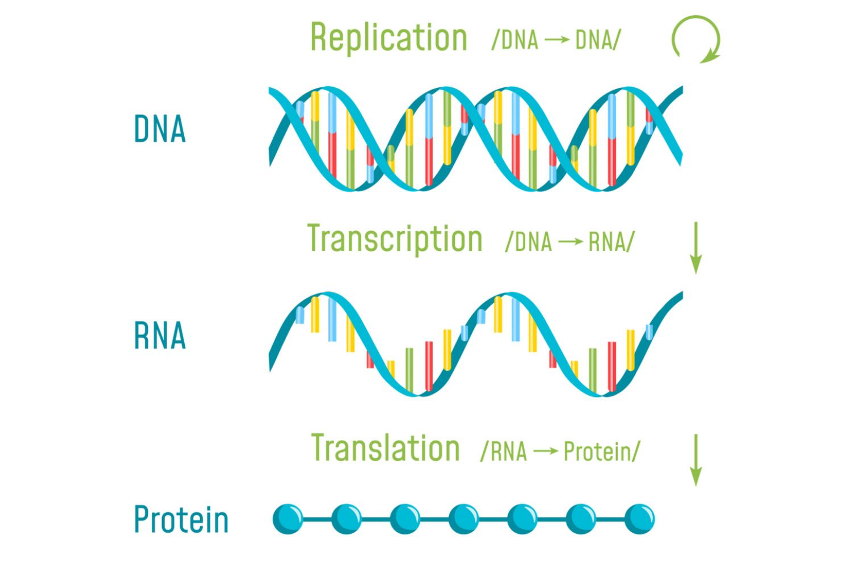
\includegraphics[width=0.5\linewidth]{\toplevelprefix/chapters/chapter1/figs/DNAs.png}
%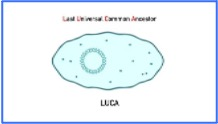
\includegraphics[width=0.28\linewidth]{\toplevelprefix/chapters/chapter1/figs/Luca.jpg}
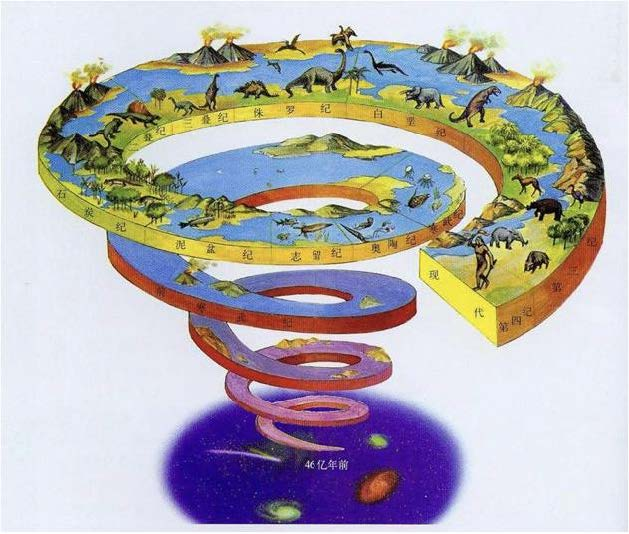
\includegraphics[width=0.40\linewidth]{\toplevelprefix/chapters/chapter1/figs/Evolution.jpg}
    \caption{Evolution of phylogenetic intelligence: Knowledge of the external world is encoded and passed on via DNAs (left), and it is decoded from DNA to RNA and to Protein etc. In the early stage of life evolution (right), intelligence develops knowledge at the species level via (random) gene mutation and natural selection -- ``may the fittest survive,'' which can be viewed as a primitive form of reinforcement learning.}
    \label{fig:phylogenetic}
\end{figure}
\begin{figure}
    \centering
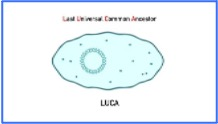
\includegraphics[height=0.19\linewidth]{\toplevelprefix/chapters/chapter1/figs/Luca.jpg}
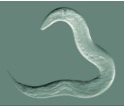
\includegraphics[height=0.19\linewidth]{\toplevelprefix/chapters/chapter1/figs/Worm.jpg}
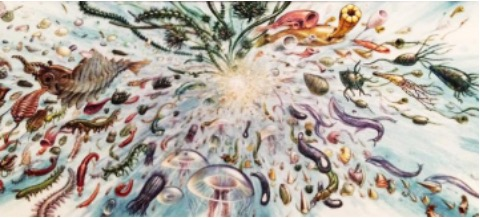
\includegraphics[height=0.19\linewidth]{\toplevelprefix/chapters/chapter1/figs/Cambrian.jpg}
    \caption{Evolution of life, from the ancestor of all life today (named LUCA --- last universal common ancestor), a single-cell-like organism which lived from 3.5-4.3 billion years ago, to the emergence of the first nervous system in worm-like species (middle), about 550 million years ago, to the explosion of life forms in the Cambrian period (right), about 530 million years ago.}
    \label{fig:evolution}
\end{figure}

{\em The ontogenetic intelligence} refers to the learning mechanisms that allow an individual to learn through its own senses, memories, and predictions within its specific living environment and to improve and adapt its behaviors. The ontogenetic learning became possible after the emergence of the nervous system about 550 to 600 million years ago (in worm-like organisms), shown in Figure \ref{fig:evolution} middle. That is, with a sensory and nervous system, an individual is capable of continuously forming and improving its own knowledge about the world, also known as a memory, in addition to what is inherited from its DNAs or genes. This capability has significantly enhanced the survival of the individual and attributed to the explosion of life forms in the Cambrian period about 530 million years ago.  Compared to phylogenetic learning, ontogenetic learning is significantly more efficient and predictable, which can be realized with the resource limit of an individual in its lifespan.

Notice that both types of learning mechanisms rely on some form of feedback (from the external environment), in terms of a penalty (death) or reward (food), of a species or individuals' actions\footnote{Gene mutation of the species or actions made by the individual.} to learn. As a result, all intelligent beings, as species or as individuals, rely on a closed-loop feedback mechanism to learn and improve their knowledge about the world. We also notice that from plants, to fish, to birds, and to mammals, more advanced species rely more and more on their ontogenetic learning capabilities. They stay with and learn from their parents longer and longer after birth, because individuals of the same species need to survive in very diverse environments. 

\paragraph{Evolution of human intelligence.}
Since the emergence of homo sapiens about 315 thousand years ago, a new and higher form of intelligence emerged which evolves more efficiently and economically. Languages, first spoken\footnote{It was believed that Sanskrit was the first spoken language, dated as back as 5000 BC.} and then written\footnote{Sumerian language is believed to be one of the oldest written language in existence, first attested about 3100 BC in southern Mesopotamia.}, were developed a few thousand years ago. See Figure \ref{fig:human-intelligence}. This allows individuals to communicate and share useful information with others. Therefore, a human community or society can behave like a single intelligent organism that can learn much faster and hold more knowledge than any individual. In a way, written languages, or texts, play a role similar to DNAs and genes as they allow human societies to accumulate and pass knowledge of the world onto next generations. We may refer to this type of intelligence as {\em  societal intelligence}, to distinguish it from the phylogenetic intelligence of species and the ontogenetic intelligence of individuals. This type of knowledge accumulation serves as the foundation of ancient civilizations.
\begin{figure}
    \centering
    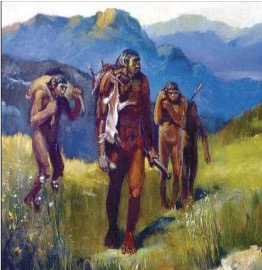
\includegraphics[height=0.25\linewidth]{\toplevelprefix/chapters/chapter1/figs/Spoken-language.jpg}
   \hspace{5mm} 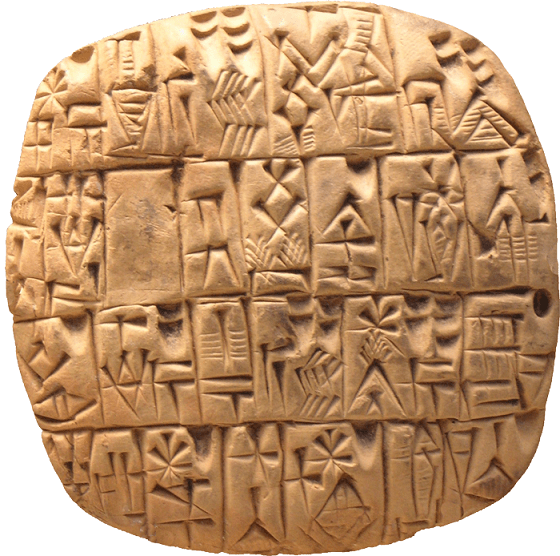
\includegraphics[height=0.25\linewidth]{\toplevelprefix/chapters/chapter1/figs/Cuneiform.png}
   \hspace{5mm} 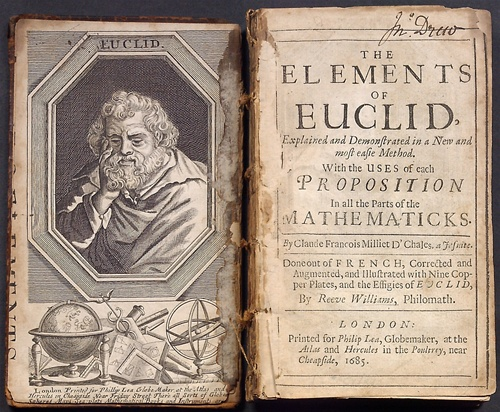
\includegraphics[height=0.25\linewidth]{\toplevelprefix/chapters/chapter1/figs/adopt-euclid1685-2.jpg}
    \caption{The development of verbal communication and spoken languages (between 10000-5000 BC), written languages (about 3000 BC), and mathematics (around 500-300 BC) mark three key milestones in the evolution of human intelligence.}
    \label{fig:human-intelligence}
\end{figure}

Quite miraculously, about a few thousand years ago, another quantum leap in human intelligence occurred, which allowed philosophers and mathematicians to develop knowledge that seem to go way beyond developing empirical knowledge. The development of abstract mathematical concepts and symbols, such as numbers, space and time, as well as mathematical logic, serve as a new precise language for modern science. In addition, the development of the ability to generate new hypotheses and verify their correctness based on  logic deduction or scientific experimentation. This, for the first time, has enabled humans to proactively develop new knowledge beyond passive empirical means. The ability to conduct these high-level forms of knowledge development is believed to be unique to humans. This advanced form of intelligence is referred to as ``artificial intelligence'' (AI), coined by John McCarthy at the Dartmouth summer workshop in 1956. 

Hence, from what we can learn from the nature, from now on, whenever we use the word ``intelligence,'' we need to be very specific about which level/form of intelligence we mean:
\begin{equation}
\mbox{\textbf{phylogentic}} \;
   \Longrightarrow \; \mbox{\textbf{ontogenetic}} \; \Longrightarrow \; 
   \mbox{\textbf{societal}}
   \; \Longrightarrow \; 
   \mbox{\textbf{artificial intelligence}}.
\end{equation}
A clear characterization and distinction are necessary and important because we want to study intelligence as a scientific and mathematical subject. It is highly likely that, even if they all may share the common objective of learning useful knowledge of the world, the specific computational mechanisms and physical implementations behind each level/form of intelligence could be different. We believe that the reader would better understand and appreciate these differences after having finished study this book. Therefore, we will leave more discussions to the last Chapter \ref{ch:future}.


%Within the realm of biology, Lorenz and Tinbergen, who were pioneers in studying animal behavior (though not intelligence per se). In cognitive science, there is a long history, including behaviorists (reinforcement learning), Gestalt psychologists etc.

%Inspiration from Science. A biography of Norbert Wiener: ``Dark Hero of the Information Age: In Search Of Norbert Wiener--Father of Cybernetics'' by Conway and Siegelman. Connections to many biologists. Wiener studied zoology as a student.


\paragraph{Origin of machine intelligence -- Cybernetics.}
In 1940s, partly due to the war effort, intelligence in nature had inspired scientists in the 1940s to emulate animal intelligence by machines, which led to the ``Cybernetics''  movement advocated by Norbert Wiener. Wiener studied zoology at Harvard as an undergraduate but later became a mathematician and control theorist. Wiener had a life long passion in understanding and developing autonomous systems that could emulate intelligent behaviors of animals. Today, the Cybernetics program is often narrowly interpreted by people as mainly about feedback control systems for which Wiener indeed made his most significant technical contributions. But the Cybernetics program was much broader and deeper than that. It is more about understanding intelligence as a whole\footnote{At least at the level of animals.} and had actually influenced the work of a whole generation of renowned scientists, including Warren McCulloch, Walter Pitts, Claude Shannon, John von Neumann, and Alan Turing.  

\begin{figure}
    \centering
    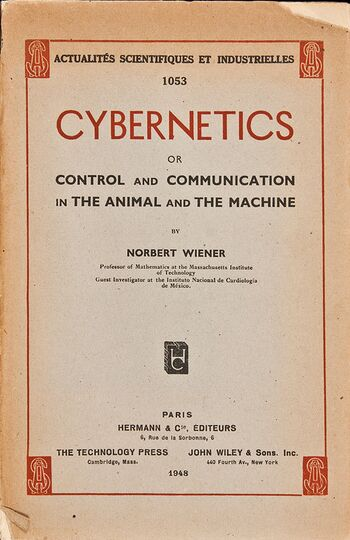
\includegraphics[height=0.4\linewidth]{\toplevelprefix/chapters/chapter1/figs/Cybernetics1.jpg}
    \hspace{10mm} 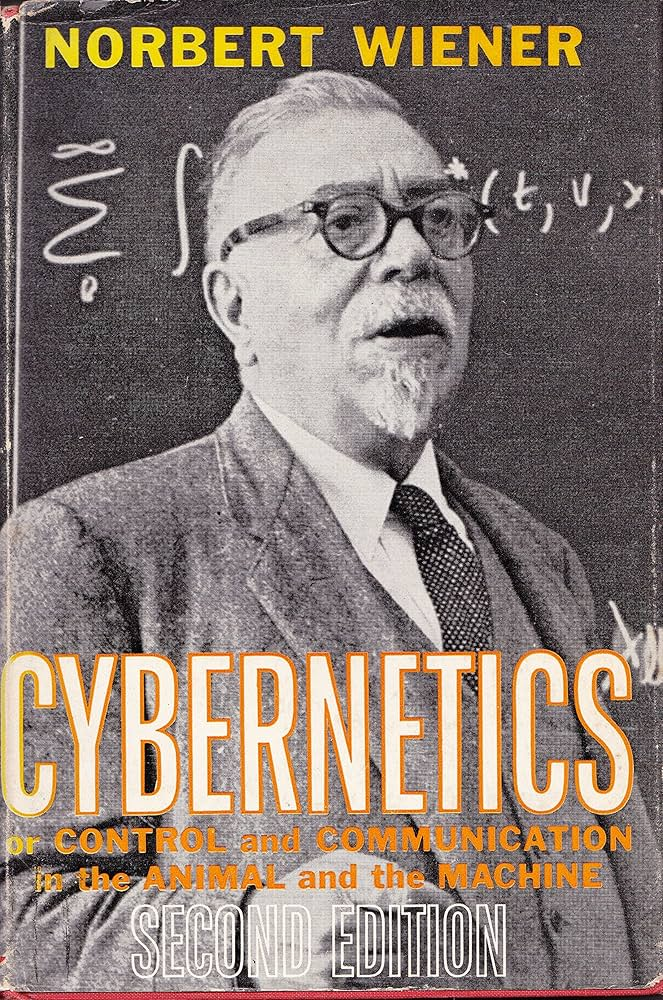
\includegraphics[height=0.4\linewidth]{\toplevelprefix/chapters/chapter1/figs/Cybernetics2.jpg}
    \caption{The book ``Cybernetics'' by Norbert Wiener published in 1948 \cite{Wiener-Cybernetics-1948} (left) and the second edition in 1961 \cite{Wiener-Cybernetics-1961} (right).}
    \label{fig:cybernetcis}
\end{figure}


Wiener was arguably the first person who studied intelligence as {\em a system}, instead of paying attention to only one component or aspect of it. His comprehensive views on intelligence were elaborated in his famous 1948 book {\em ``Cybernetics: or Control and Communication in the Animal and the Machine''} \cite{Wiener-Cybernetics-1948}. In this book and its second edition published in 1961 \cite{Wiener-Cybernetics-1961} (see Figure \ref{fig:cybernetcis}), he tried to identify several necessary characteristics and mechanisms of intelligent systems, which include (but are not limited to):
\begin{itemize}
    \item How to {\em measure and store} information (in the brain) and how to communicate with others. \footnote{Norbert Wiener was the first to point out ``information'' is not matter nor energy, but an independent quantity for study.} This led to the formulation of information theory and coding theory by Claude Shannon in 1948.
    \item How to {\em correct errors}  in prediction and estimation based on existing information. Norbert Wiener himself helped formalize the theory for control systems based on closed-loop feedback in the 1940s. 
    \item How to learn to {\em make better decisions} from interacting with a potentially non-cooperative opponent or adversarial environment. This was formalized by John von Neumann as game theory in 1944. 
\end{itemize}
In 1943, very much motivated by Wiener's Cybernetics program, the psychiatrist Warren McCulloch and the logician Walter Pitts together formalized the first computational model for a neuron \cite{McCulloch-Pitts}, called {\em an artificial neuron}, as illustrated later in Figure \ref{fig:neuron}. Based on this model, in 1950s, Frank Rosenblatt built a physical machine, named the {\em Mark I Perceptron}, with a network of hundreds of such artificial neurons. Perceptron was the first artificial neural network physically realized, see Figure \ref{fig:perceptron}. Notably, John von Neumann's universal computer architecture, proposed in 1945, was also designed to facilitate the goal of building {\em computing machines} that can physically realize the mechanisms suggested by the Cybernetics program. 

Acute readers probably have noticed that the 1940s was truly a magical era: So many fundamental ideas were invented and influential theories formalized in that era, including the mathematical model of neurons, artificial neural networks, information theory, control theory, game theory, and computing machines. Figure \ref{fig:god-fathers} shows some of the pioneers of these theories. As we now know, each work above had grown to become the foundation of a scientific or engineering field for the following many decades and has tremendous impact on us. All these fundamental theories were inspired and motivated by the goal of trying to develop machines that can emulate intelligence in nature. Based on historical notes, Wiener's Cybernetics movement had influenced almost all of these people and work. 
\begin{figure}
    \centering
    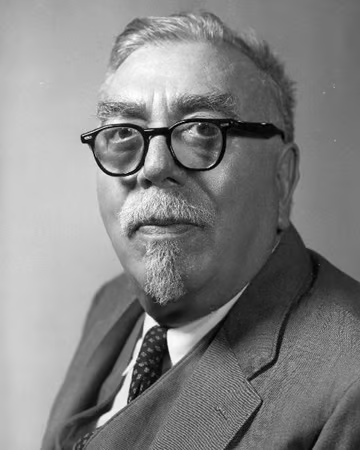
\includegraphics[height=0.3\linewidth]{\toplevelprefix/chapters/chapter1/figs/Wiener.png}
    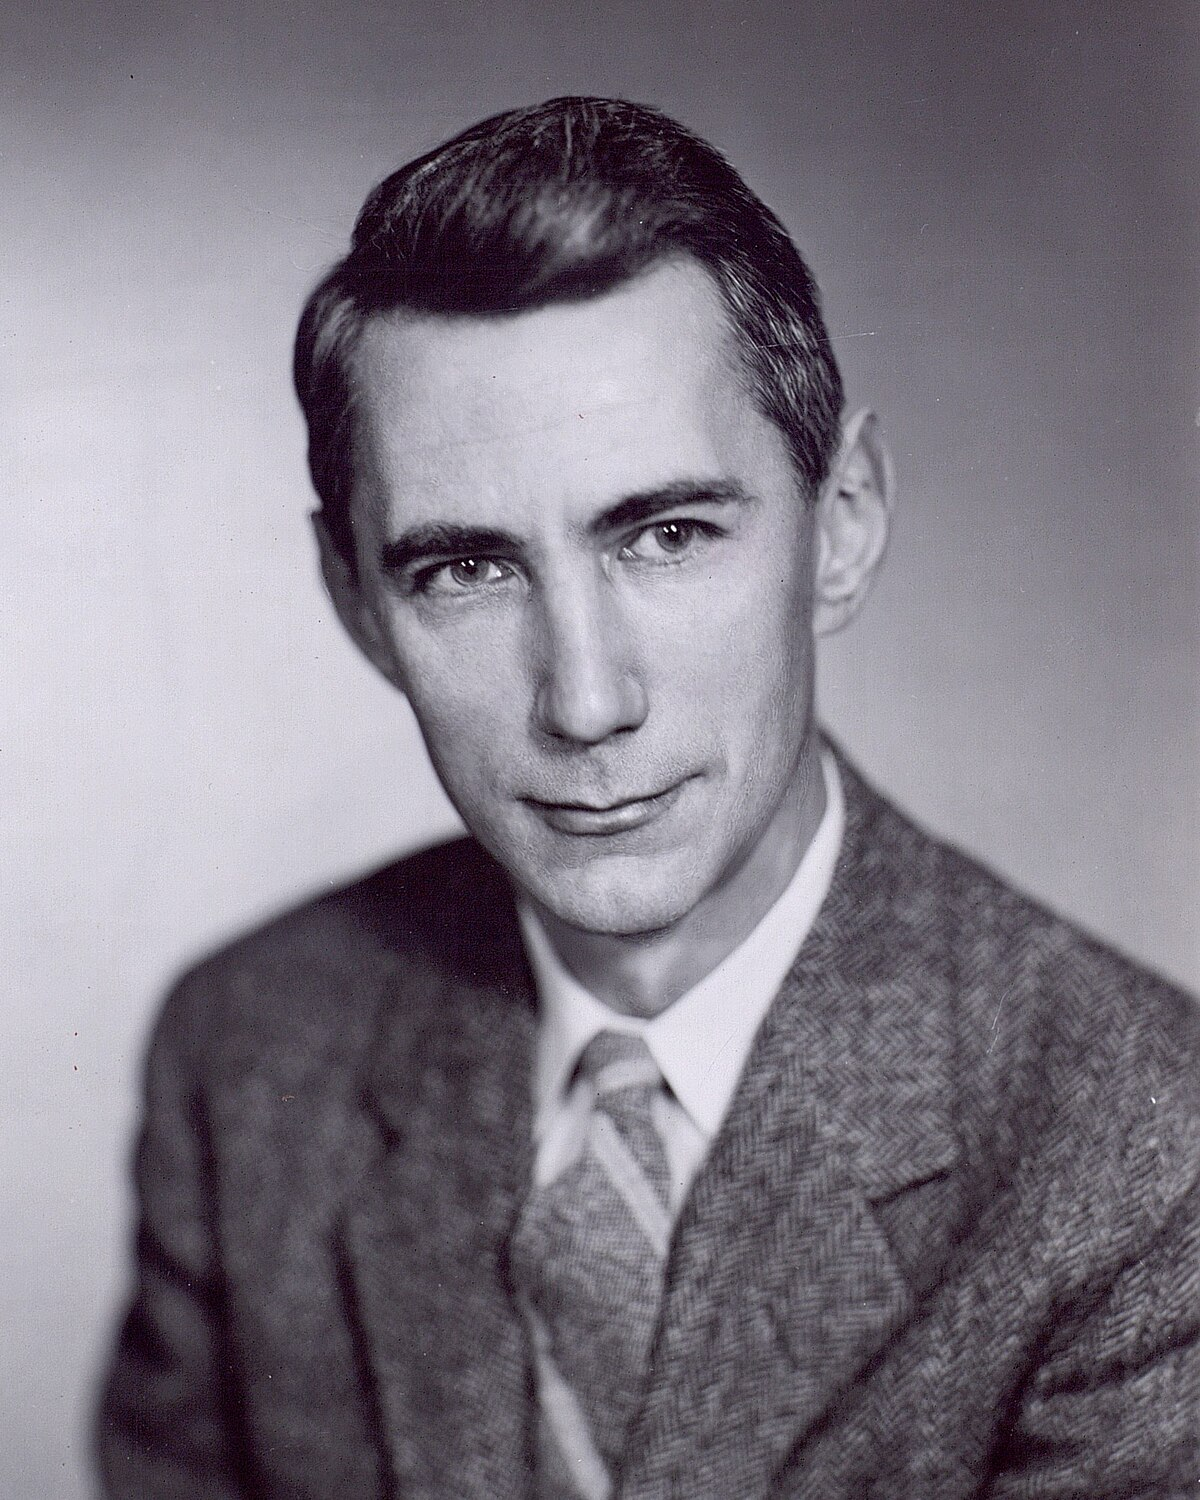
\includegraphics[height=0.3\linewidth]{\toplevelprefix/chapters/chapter1/figs/Shannon.jpg}
    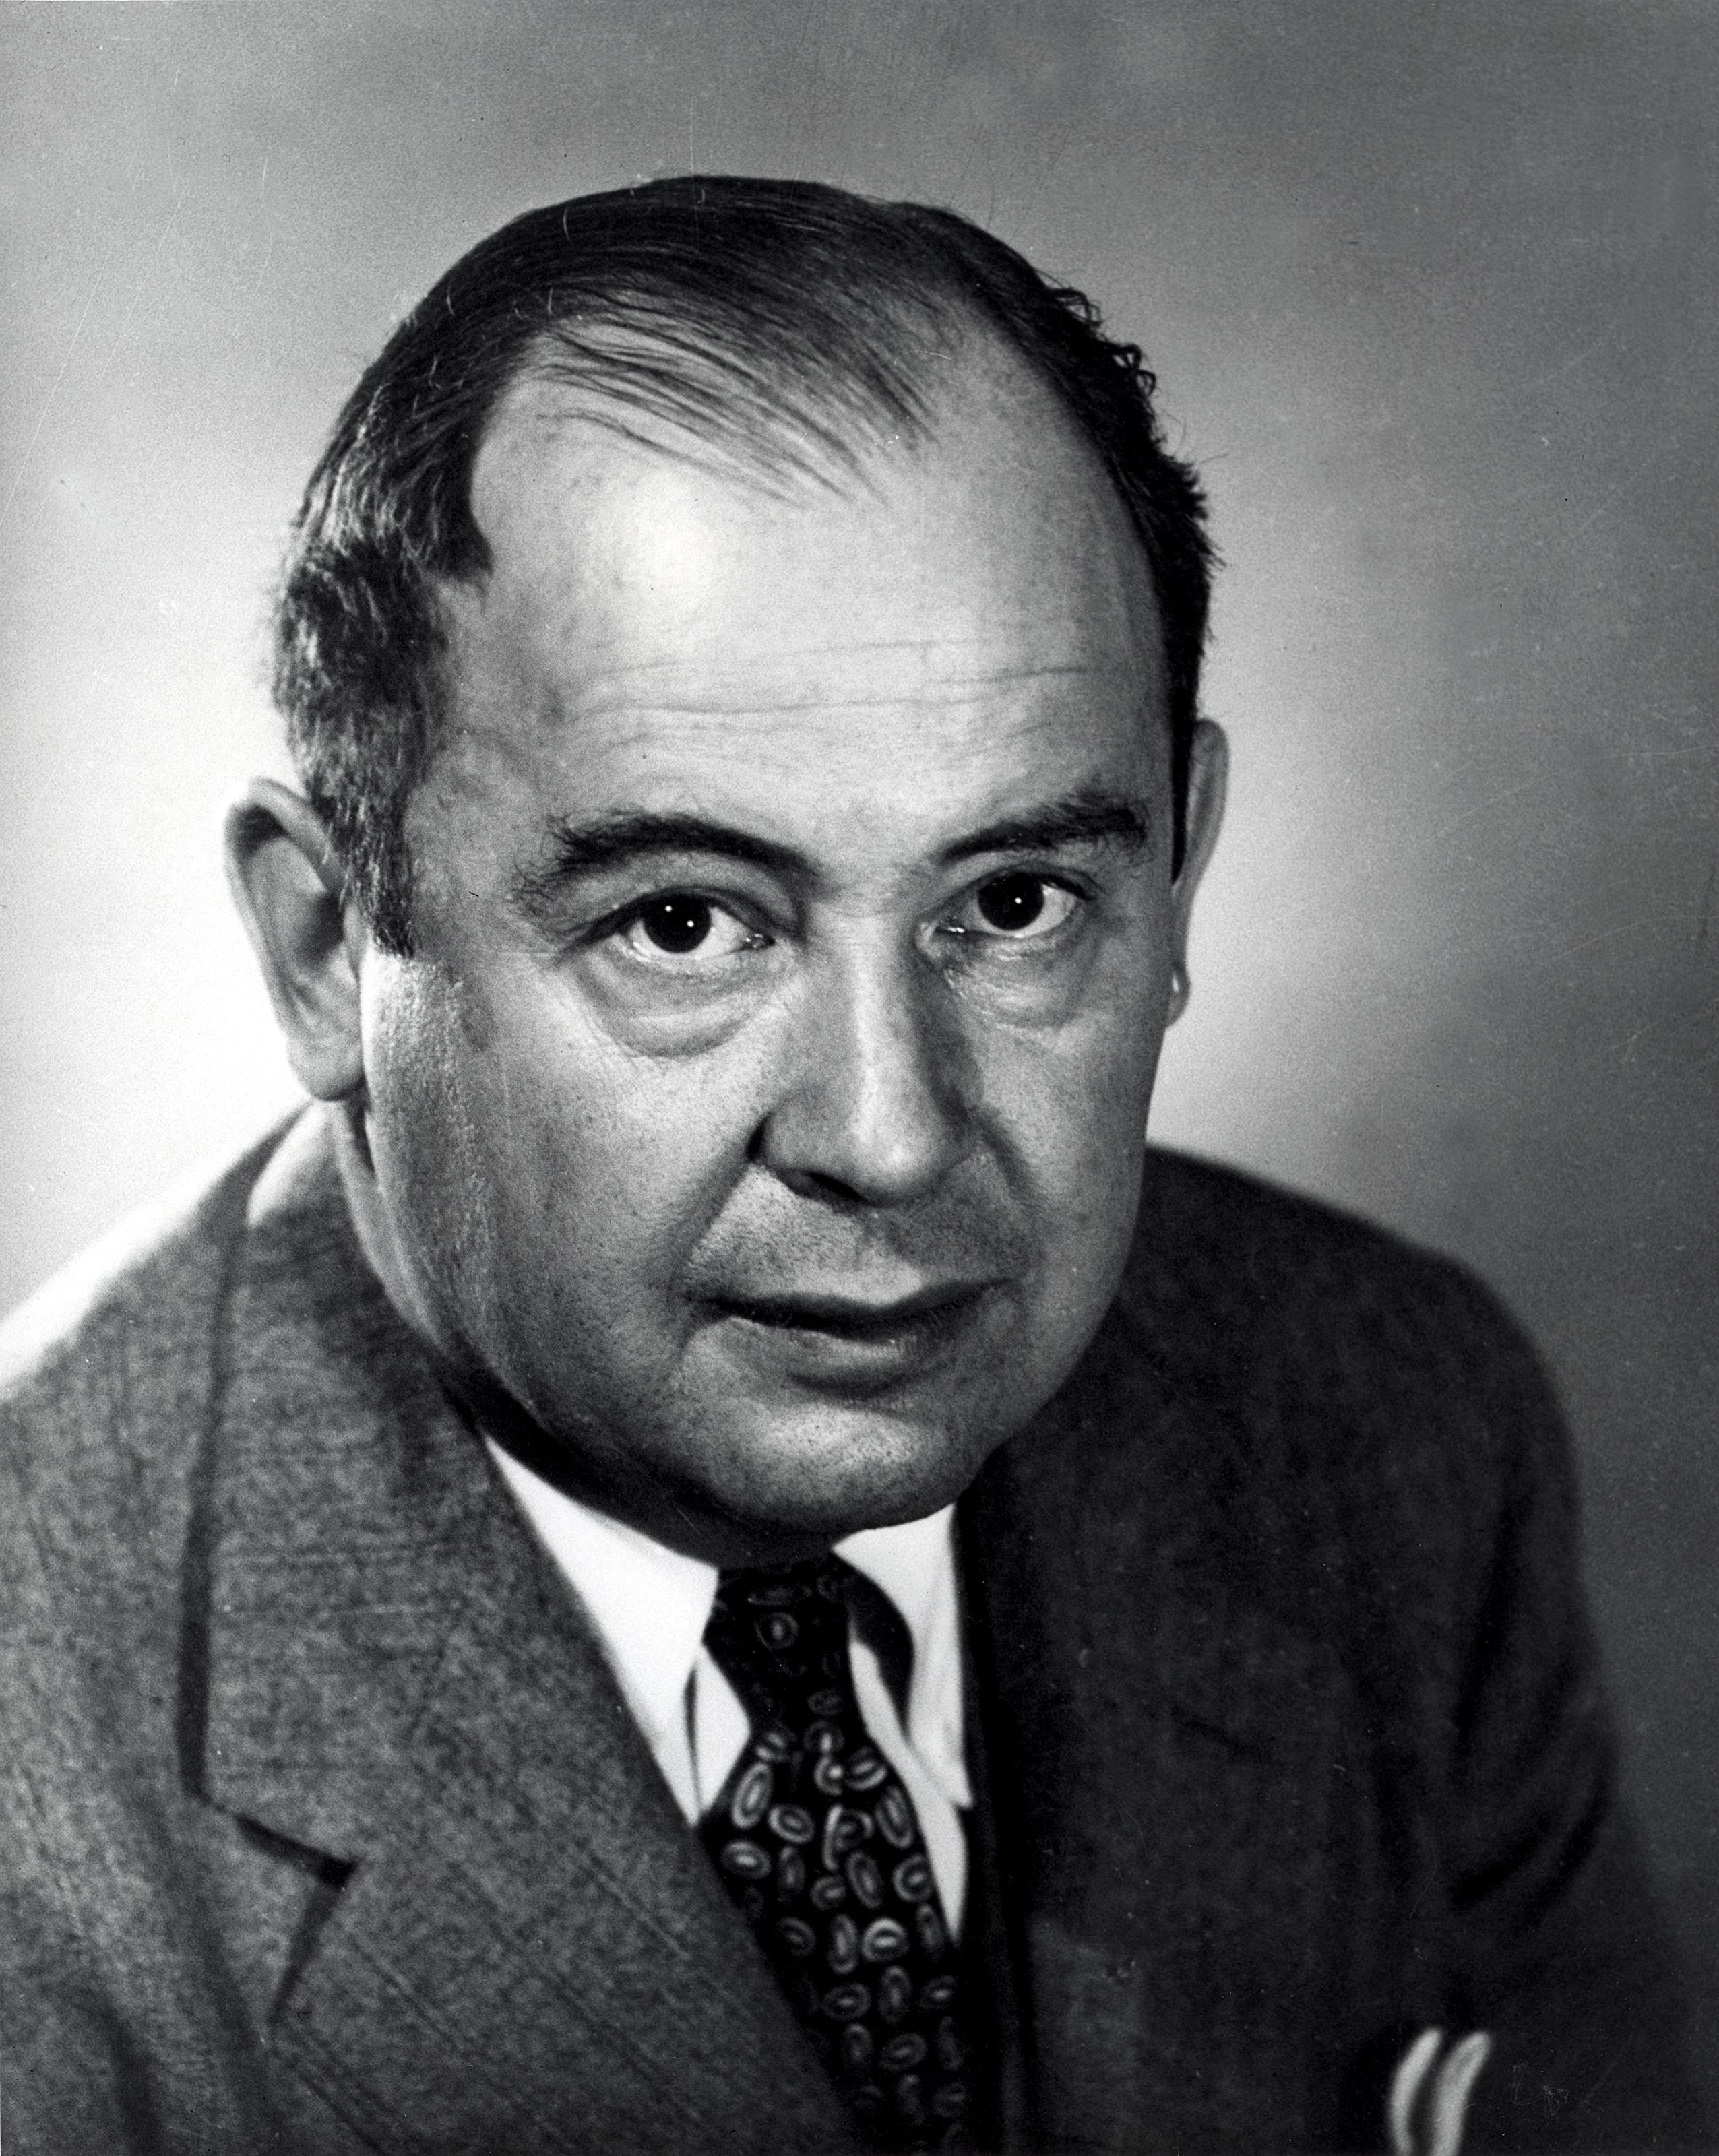
\includegraphics[height=0.3\linewidth]{\toplevelprefix/chapters/chapter1/figs/neumann.jpg}
    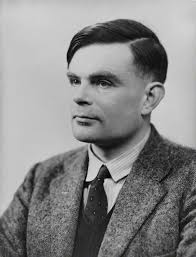
\includegraphics[height=0.3\linewidth]{\toplevelprefix/chapters/chapter1/figs/Turing.jpeg}
    \caption{Pioneers of theoretical and computational foundations for intelligence: Norbert Wiener (cybernetics and control theory), Claude Shannon (information theory), John von Neumann (game theory), and Alan Turing (computing theory).}
    \label{fig:god-fathers}
\end{figure}

Although Wiener in his work had identified many key characteristics and mechanisms of intelligence, there was no indication that he knew how to properly integrate all these mechanisms together to build a complete autonomous intelligent system. Judging from today's knowledge, some of his views on these mechanisms were not entirely accurate or complete. In particular, in the last chapter of the second edition of Cybernetics \cite{Wiener-Cybernetics-1961}, he pointed out that it is crucial to {\em deal with nonlinearality} if a machine learning system is designed to emulate typical learning mechanisms in nature. But he did not provide any concrete and effective solutions to this difficult issue. To his defense though, at the time, few people knew how, since even the theory for dealing with linear models and systems was still in its infancy. 

Nevertheless, we could not help but marvel at Wiener's foresight about the importance of nonlinearity. As we will see in this book, the answer was found only recently: nonlinearity can be effectively dealt with through progressive linearization and transformation realized by deep neural networks (see Chapter \ref{ch:representation}). In addition, we will attempt to show in this book how all these mechanisms listed above can be naturally integrated into a complete system which would exhibit characteristics of an autonomous intelligent system (see Chapters \ref{ch:autoencoding} and \ref{ch:closed-loop}). 

\paragraph{Origin of Artificial Intelligence.}
From the subtitle of Wiener's Cybernetics book: {\em ``Control and Communication in the Animal and the Machine''}, one can tell that the studies in the 1940s mainly aimed to emulate intelligence at the level of animals. As we mentioned before, the research agendas about intelligence around the 1940s were very much dominated by Norbert Wiener's Cybernetics movement. 

Alan Turing was one of the first to notice this limitation. In his famous 1950 paper ``{\em Computing Machinery and Intelligence}'' \cite{Turing-1950}, Turing formally posted the question whether machines can imitate intelligence even at the human level, to the point of being indistinguishable from the intelligent capabilities of humans. This is now known as {\em the Turing test}. 

Around 1955, a group of young and ambitious scientists tried to break away from the then dominating Cybernetics movement and research agendas so that they would have a chance to create their own legacy. They decided to take on Turing's challenge of imitating human intelligence and proposed a workshop to be held at Dartmouth College in the summer of 1956. They made their intention clear with a statement in their proposal: 
\begin{quote}
    ``{\em The study is to proceed on the basis of the conjecture that every aspect of learning or any other feature of intelligence can in principle be so precisely described that a machine can be made to simulate it. An attempt will be made to find how to make machines use language, form abstractions and concepts, solve kinds of problems now reserved for humans, and improve themselves}.'' 
\end{quote}
In essence, they wanted to formalize and study higher-level intelligence that differentiates humans from animals. The topics they considered ranged from abstraction, symbolic methods, natural languages, and deductive methods (including causal inference, logic deduction, etc.) The organizer of the workshop, John McCarthy, then a young assistant professor of Mathematics of the Dartmouth College, coined the now famous term ``Artificial Intelligence'' (AI) to encapsulate the set of characteristics or mechanisms that are believed to be {\em unique to human intelligence}. 

\paragraph{The renaissance of ``Artificial Intelligence'' or ``Cybernetics''?}
As the readers may have known, in the past decade or so, machine intelligence has undergone explosive development, powered mainly by the practice of deep artificial neural networks, triggered by the work of Geoffrey Hinton and students in 2012 \cite{krizhevsky2012imagenet}. This era is also hailed as the ``Renaissance'' of Artificial Intelligence (AI). However, in terms of tasks that people have actually tried to tackle (recognition, generation, and prediction) and techniques that people have developed and implemented so far (reinforcing, imitating, encoding, decoding, denoising, and compression), we are very much just emulating the mechanisms that are common to the intelligence of early life and animals. Even in that regard, as we will try to clarify in this book, current ``AI'' models and systems have not correctly implemented all necessary mechanisms for intelligence at these levels, which were already known to the Cybernetics movement in the 1940s. 

Hence, strictly speaking, the advancement of machine intelligence in the past decade does not align well with the ``Artificial Intelligence'' program laid out in the 1956 Dartmouth workshop. Instead, what has been predominantly accomplished so far is more closely related to the objectives of the classic ``Cybernetics'' program laid out by Norbert Wiener in the 1940s. It is probably more appropriate to call the current era the ``Renaissance of Cybernetics''.\footnote{The recent rise of the so-called ``Embodied AI'' for autonomous intelligent robots share even more similarity with the goals of the Cybernetics program.} Only after we have fully understood what we have truly done from the scientific and mathematical perspective, can we truly know what remains to be done and which direction to go to pursue the true nature of intelligence. This is one of the main purposes of this book. 


\section{What to Learn?}
\label{sec:what-to-learn}
%Notes: The notion of intelligence can be very  general and broad. But that often makes it ambiguous. Here, we here try to give a more precise description about what it mainly is. Our definition may have significantly narrowed the scope, but make it more implementable, verifiable, and even measurable (via computable means). 



\subsection{Predictability}
\label{sec:predictability}
Data that carry useful information manifest in many different forms. In the most natural form, they can be modeled as sequences that are predictable and computable. The notion and properties of a predictable and computable sequence were at the heart of the theory of computing and very much led to the invention of computers \cite{Turing-1936}. The role of predictable sequences in (inductive) inference was studied by Ray Solomonoff, Andrey Kolmogorov, and many others in the 1960s \cite{Kolmogorov1998OnTO} as a generalization to Claude Shannon's classic Information Theory \cite{Shannon-1948}. To understand the concept of predictable sequences, let us first start with some concrete simple examples. 
\paragraph{Scalar Case.} The simplest predictable discrete sequence is arguably the sequence of natural numbers:
\begin{equation}
   {S} =  1, 2, 3, 4, 5, 6, \ldots, n, n+1, \ldots
\end{equation}
in which the next number $x_{n+1}$ is defined to be its previous number $x_n$ plus 1:
\begin{equation}
x_{n+1} = x_n + 1.    
\end{equation}
One may generalize the notion of predictability to any sequence $\{x_n\}_{n=1}^\infty$ with $ x_n \in \mathbb{R}$ if the next number $x_{n+1}$ can always be computed from its previous one $x_n$:
\begin{equation}
    x_{n+1} = f(x_{n}), \quad x_n \in \mathbb{R}, \; n =  1, 2, 3, \ldots
\end{equation}
where $f(\cdot)$ is a {\em computable} (scalar) function.\footnote{Here we emphasize that the function $f(\cdot)$ itself is computable, say it can be implemented as a program on a computer. } Note that here we emphasize that the function $f(\cdot)$ must be computable. There are many functions that can be defined but are not computable. Alan Turing's seminal work in 1936 \cite{Turing-1936} gives a rigorous definition of computability. In practice, we often further assume that $f$ is efficiently computable and has nice properties such as being continuous and differentiable, etc. The necessity of these properties will become clear later once we understand more about more refined notions of computability, and their roles in machine learning and intelligence.

\paragraph{Multi-Variable Case.}
Of course, the value of the next number can also depend on two of its predecessors. For example, the famous {\em Fibonacci sequence} is defined to be:
\begin{equation}
    {S} = 1, 1, 2, 3, 5, 8, 13, 21, 34, 55, \ldots
\end{equation}
where one can easily see:
\begin{equation}
    x_{n+2} = x_{n+1} + x_{n}, \quad  x_n \in \mathbb{R}, \;  n = 1, 2, 3, \ldots
\end{equation}
Similarly, we may generalize this recursion to \begin{equation}
    x_{n+2} = f(x_{n+1}, x_{n}), \quad x_n \in \mathbb{R}, \;  n =  1, 2, 3, \ldots
\end{equation}
where $f(\cdot,\cdot)$ is any computable function that takes two variables as input. We can further generalize the notion of predictability to a sequence whose next value depends on say $d$ of its predecessors:
\begin{equation}
    x_{n+d} = f(x_{n+d-1}, \ldots,  x_{n}), \quad  x_n \in \mathbb{R}, \; n =  1, 2, 3, \ldots
    \label{eqn:recursive-d}
\end{equation}
The number of predecessors $d$ needed for the prediction is called the {\em degree} of the recursive prediction. The above expression \eqref{eqn:recursive-d} is also called an {\em (auto) regression}. Such a sequence is also called a {\em auto-regressive} sequence. If the function $f$ is a linear function, we call it a linear (auto) regression. 

\paragraph{Vector Case.} 
To simplify the notation, we may define a vector $\vx \in \mathbb{R}^d$ that collects $d$ consecutive values in the sequence  \begin{equation}
    \vx_n \doteq [x_{n+d-1}, \ldots,  x_{n}]^\top, \quad \vx_n \in \mathbb{R}^d, \; n = 1, 2, 3, \ldots
\end{equation}
With this notation, the recursive relation \eqref{eqn:recursive-d} can be conveniently written as
\begin{equation}
    \vx_{n+1} = g(\vx_{n}) \; \in \mathbb{R}^d, \quad n =  1, 2, 3, \ldots
    \label{eqn:recursive-v}
\end{equation}
where the function $g(\cdot)$ is uniquely defined by the function $f$ in \eqref{eqn:recursive-d} and it  takes a $d$-dimensional vector as input. In different contexts, such a vector is sometimes referred to as a ``state'' or a ``token''. Note that the equation in \eqref{eqn:recursive-d} denotes a mapping $\mathbb{R}^d \rightarrow \mathbb{R}$, but the equation here is $g: \mathbb{R}^d \rightarrow \mathbb{R}^d$.


\paragraph{Controlled Prediction.}
We may also define a predictable sequence that depends on another predictable sequence as input:
\begin{equation}
    \vx_{n+1} = f(\vx_{n}, \vu_n) \; \in \mathbb{R}^d, \quad n =  1, 2, 3, \ldots,
\label{eqn:recursive-control}
\end{equation}
where $\{\vu_n\}$ with $\vu_n \in \mathbb{R}^k$ is a (computable) predictable sequence. In other words, the next vector $\vx_{n+1} \in \mathbb{R}^d$ depends on both $\vx_n \in \mathbb{R}^d$ and $\vu_n \in \mathbb{R}^k$. In the context of control theory, the sequence $\{\vu_n\}$ is often referred to as the ``control input'' and  $\vx_n$ as the ``state'' or ``output'' of the system \eqref{eqn:recursive-control}. One classic example is a linear dynamical system:
\begin{equation}
    \vx_{n+1} = \boldsymbol{A}\vx_n + \boldsymbol{B}\vu_n, \quad \boldsymbol{A} \in \mathbb{R}^{d\times d}, \boldsymbol{B} \in \mathbb{R}^{d\times k},
    \label{eqn:lineary-system} 
\end{equation}
which is widely studied in control theory \cite{Cal:Des}. 

Very often the control input is given by a computable function of the state $\vx_n$ itself, say: 
\begin{equation}
    \vu_n = h(\vx_n), \quad n =  1, 2, 3, \ldots 
\end{equation}
As a result, the sequence $\{\vx_n\}$ is given by composing the two computable functions $f$ and $h$ as:
\begin{equation}
    \vx_{n+1} = f\big(\vx_{n}, h(\vx_n)\big), \quad n =  1, 2, 3, \ldots
    \label{eqn:recursive-closed-loop}
\end{equation}
In this way, the sequence $\{\vx_n\}$ again becomes an auto-regressive predictable sequence.  When the input $\vu_n$ depends on the output $\vx_n$, we say the resulting sequence is produced by a ``closed-loop'' system \eqref{eqn:recursive-closed-loop}. As the closed-loop system no longer depends on any external input, we say such a system has become {\em autonomous}. It can be viewed as a special case of auto-regression. For instance, if we choose in the above linear system \eqref{eqn:lineary-system}, $\vu_n = \boldsymbol{F}\vx_n$, the closed-loop system becomes
\begin{equation}
        \vx_{n+1} = \boldsymbol{A}\vx_n + \boldsymbol{B}\vu_n = \boldsymbol{A}\vx_n + \boldsymbol{B}\boldsymbol{F}\vx_n = (\boldsymbol{A}+ \boldsymbol{B}\boldsymbol{F})\vx_n,
    \label{eqn:lineary-system-closed}
\end{equation}
which is a linear auto-regression. 

% \paragraph{Approximate prediction.}
% What if in the above equation \eqref{eqn:recursive-control} the input sequence $\vu_n$ is not predictable? One extreme case is when it is completely unpredictable, say:
% \begin{equation}
%     \vx_{n+1} = f(\vx_{n}, \boldsymbol{\epsilon}_n), \quad n =  1, 2, 3, \ldots
%     \label{eqn:recursive-noise}
% \end{equation}
% where $\boldsymbol{\epsilon}_n \in \mathbb{R}^k$ is some random (Gaussian) noise. In such cases, we say the so-defined sequence $\{\vx_n\}$ ``stochastic''. Obviously, such a sequence is no longer fully predictable, at least not in a deterministic sense as above. 

% When magnitude of the noise  $\|\boldsymbol{\epsilon}_n\|$ is small and the function $f$ does not amplify the noise so much, we have
% \begin{equation}
%     \vx_{n+1} \approx f(\vx_{n}, \boldsymbol{0}) + \nabla_{\boldsymbol{\epsilon}}f(\vx_{n}, \boldsymbol{0})   \boldsymbol{\epsilon}_n, \quad n =  1, 2, 3, \ldots
%     \label{eqn:recursive-noise-small}
% \end{equation}
% where the magnitude of the second term $\|\nabla_{\boldsymbol{\epsilon}}f(\vx_{n}, \boldsymbol{0})   \boldsymbol{\epsilon}_n\|$ is small. Hence $ \vx_{n+1}$ is largely determined by the first deterministic term and its expectation is predictable: 
% \begin{equation}
%     \mathbb{E}[\vx_{n+1}] \approx f(\vx_{n}, \boldsymbol{0}).
% \end{equation}
% In this case, we say the sequence $\{\vx_n\}$ defined by \eqref{eqn:recursive-noise-small} is ``approximately predictable''. In practice, we often deal with this type of approximate predictability in real-world data in which  measurement noises are commonplace. Note that taking the expectation essentially removes the effect of  random noise and renders the expectation $\{\mathbb{E}[\vx_n]\}$ a predictable sequence. Such a process is typically referred to as ``denoising''. \DP{the connection between ``denoising'' here and ``denoising'' in Ch 2/3 is not obvious at first glance. For instance, here it is w.r.t.~an autoregressive sequence, but later it is for single observations. this isn't the same thing as filtering either. I don't really see why we need this paragraph (at least here).} 

\paragraph{Continuous Processes.}
Predictable sequences have their natural counterparts in the continuous case. We may refer to them as predictable processes. Similar to the sequence of natural numbers, the simplest predictable continuous process is time itself $x=t$.

More generally, we say a process, denoted by $\vx(t)$, is predictable if at any time $t$, the value of the process at $t+\delta t$, where $\delta t$ is an infinitesimal increment, is determined by its value at $t$. Typically, the change in value $\delta \vx(t)$ is continuous and smooth. So $\delta \vx(t) = \vx(t + \delta t) - \vx(t)$ is infinitesimally small.  Predictable processes are typically described by (multivariate) differential equations:
\begin{equation}
    \dot{\vx}(t) = f(\vx(t)), \quad \vx \in \mathbb{R}^d. 
    \label{eqn:process}
\end{equation}

In the context of systems theory \cite{Cal:Des,Sastry-Nonlinear}, the above equation is also known as a state-space model. Similar to the discrete case, a controlled process can be given by:
\begin{equation}
    \dot{\vx}(t) = f(\vx(t), \vu(t) ), \quad \vx \in \mathbb{R}^d, \vu \in \mathbb{R}^k,
    \label{eqn:process-controlled}
\end{equation}
where $\vu(t)$ is a computable input process. 

\begin{example}
    For example in physics, Newton's second law of motion describes how to predict the trajectory $\boldsymbol{x}(t) \in \mathbb{R}^3$ of a moving object under a force input $\boldsymbol{F}(t) \in \mathbb{R}^3$:
\begin{equation}
    m\ddot{\boldsymbol{x}}(t) = \boldsymbol{F}(t).
\end{equation}
When there is no force $\boldsymbol{F}(t) \equiv 0$, the above law reduces to a  special case, known as Newton's first law: the object maintains a constant speed in a straight line:
\begin{equation}
   \ddot{\boldsymbol{x}}(t) = \boldsymbol{0} \; \Leftrightarrow \; \dot{\boldsymbol{x}}(t) = \boldsymbol{v}
\end{equation}
for some constant velocity vector $\boldsymbol{v} \in \mathbb{R}^3$.
\end{example}




\subsection{Low Dimensionality}\label{sec:intro-low-dimensionality}
\paragraph{Learn to Predict.}
Now suppose you have observed or are given many sequence segments:
\begin{equation}
    \{S_1, S_2, \ldots, S_i, \ldots, S_N\}
\end{equation}
all from some predictable sequence $\{x_n\}_{n=1}^\infty$. Without loss of generality, we may assume the length of each segment is $D \gg d$. So each segment is of the form:
\begin{equation}
    S_i = [x_{j(i)}, x_{j(i)+1}, \ldots, x_{j(i)+D-1}]^\top \in \mathbb{R}^D
\end{equation}
for some $j \in \mathbb{N}$. Then you are given a new segment $S_t$ and are asked to predict its future values. 

One difficulty here is that you normally do not know the function $f$ and the degree $d$ from which the sequence is generated: 
\begin{equation}
    x_{n+d} = f(x_{n+d-1}, \ldots,  x_{n}).
\label{eqn:sequence-order-d}
\end{equation}
So the hope is somehow ``to learn'' $f$ and $d$ from the given sample segments $S_1, S_2, \ldots, S_N$. Hence the central task of learning to predict is:
\begin{center}
{\em Given many sampled segments of a predictable sequence, how to effectively and efficiently identify the function $f$.}
\end{center}

\paragraph{Predictability and Low-Dimensionality.}
To identify the predictive function $f$, we may notice a common characteristic of segments of any predictable sequence, say given by \eqref{eqn:sequence-order-d}. If we take a long segment, say with a length $D \gg d$, of the sequence and view it as a vector: 
\begin{equation}
    \vx_i = [x_i, x_{i+1}, \ldots x_{i+D-1}]^\top \in \mathbb{R}^D.
\end{equation}
Then the set of all such vectors $\{\vx_i\}$ are far from random and hence cannot possibly occupy the entire space of $\R^D$. Instead, they essentially have at most $d$ degrees of freedom -- given the first $d$ entries of any $\vx_i$, values of the rest of the entries are uniquely determined. In other words, all $\{\vx_i\}$ lie on a $d$-dimensional surface. In mathematics, such a surface is often called a submanifold, denoted as $\mathcal{S} \subset \R^D$.


\begin{figure}[t]
\centering
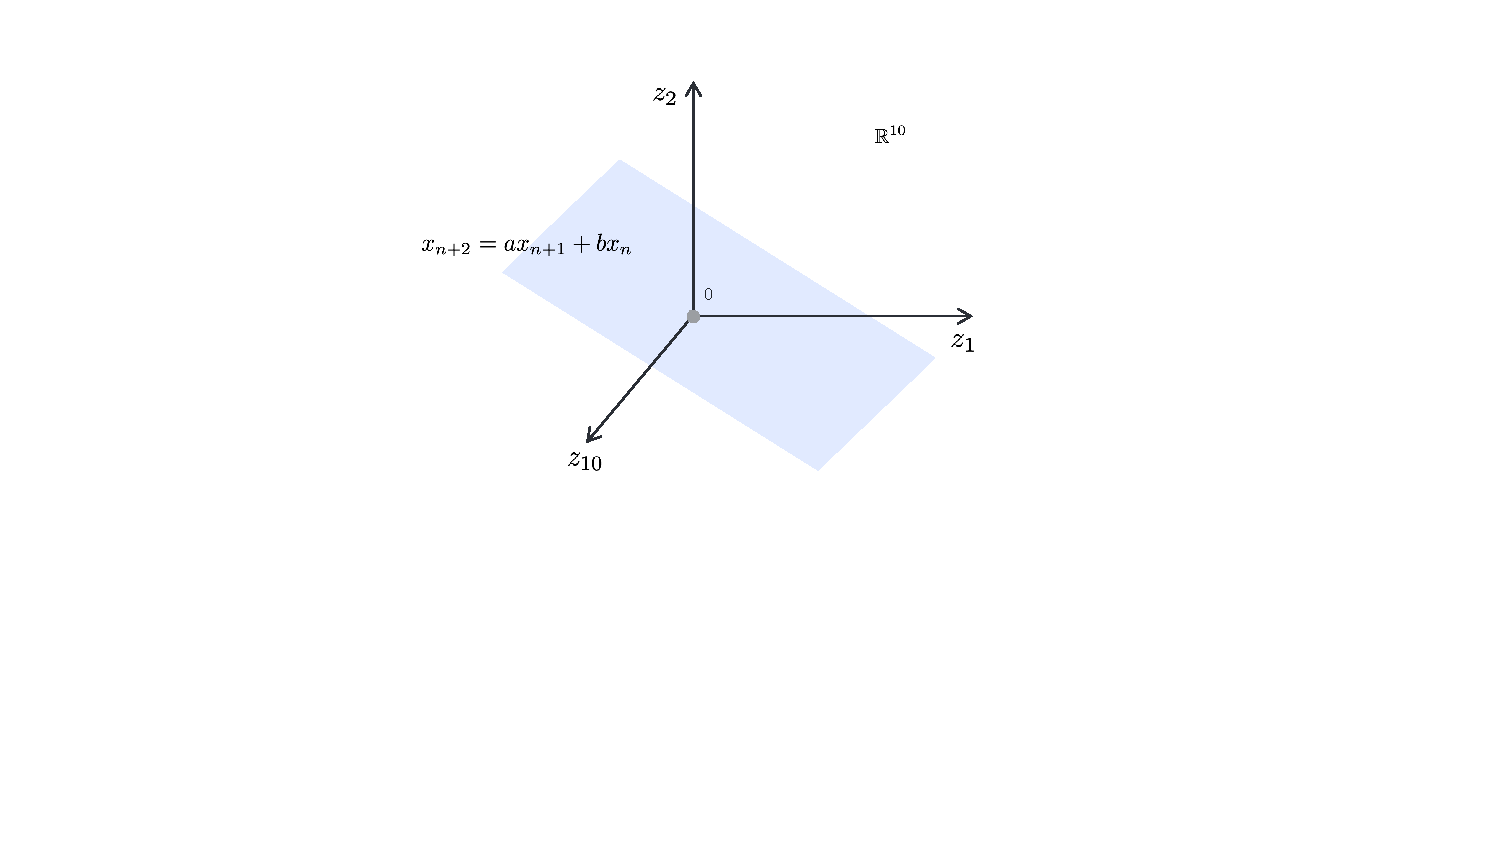
\includegraphics[width=0.6\linewidth]{\toplevelprefix/chapters/chapter1/figs/two-dimensional plane in R10.pdf}
    \caption{A two-dimensional subspace in a ten-dimensional ambient space.}
    \label{fig:lowdimplane}
\end{figure}
In practice, if we choose the segment length $D$ to be large enough, then all segments sampled from the same predicting function lie on a surface with an intrinsic dimension $d$, significantly lower than that of the ambient space $D$. For example, if the sequence is given by the following linear autoregression:
\begin{equation}
    x_{n+2} = a\cdot x_{n+1} + b\cdot x_n,
    \label{eqn:sequence-2d}
\end{equation}
for some constants $a, b \in \R$. If we sample segments of length $D =10$ from such a sequence, then all samples lie on a two-dimensional plane or subspace in $\R^{10}$, as illustrated in Figure \ref{fig:lowdimplane}. If we can identify this two-dimensional subspace, the constants $a$ and $b$ in \eqref{eqn:sequence-2d} can be fully determined. 


It is easy to see that if the predicting function $f$ is linear, such as the case with the linear systems given in \eqref{eqn:lineary-system} and \eqref{eqn:lineary-system-closed}, the long segments always lie on certain low-dimensional linear subspace. Identifying the predicting function is largely equivalent to identifying this low-dimensional subspace, a problem generally known as principal component analysis. We will discuss such classic models and methods in Chapter \ref{ch:classic}.

As it turns out, this is largely true for general predictable sequences too: if one can identify the low-dimensional surface on which all the segment samples lie, then one can identify the associated predictive function $f$.\footnote{Under mild conditions, there is a one-to-one mapping between the low-dimensional surface and the function $f$. This fact has been exploited in problems such as system identification which we will discuss later.} We cannot over-emphasize the importance of this property of segments from a predictable sequence: {\em All samples of long segments of a predictable sequence lie on a low-dimensional submanifold.} As we will see in this book, all modern learning methods essentially exploit this property, implicitly or explicitly. %\yima{Add a Figure to illustrate the surface or submanifold.} 

In real-world scenarios, the data we observe often do not come from a single predictable sequence. Typically they contain observations of multiple predictable sequences. For example, a video sequence can contain multiple moving objects. It is easy to see that in such scenarios, the data lie on a mixture of multiple low-dimensional linear subspaces or nonlinear submanifolds, as illustrated in \Cref{fig:mixture-models}. 
\begin{figure}
    \centering
    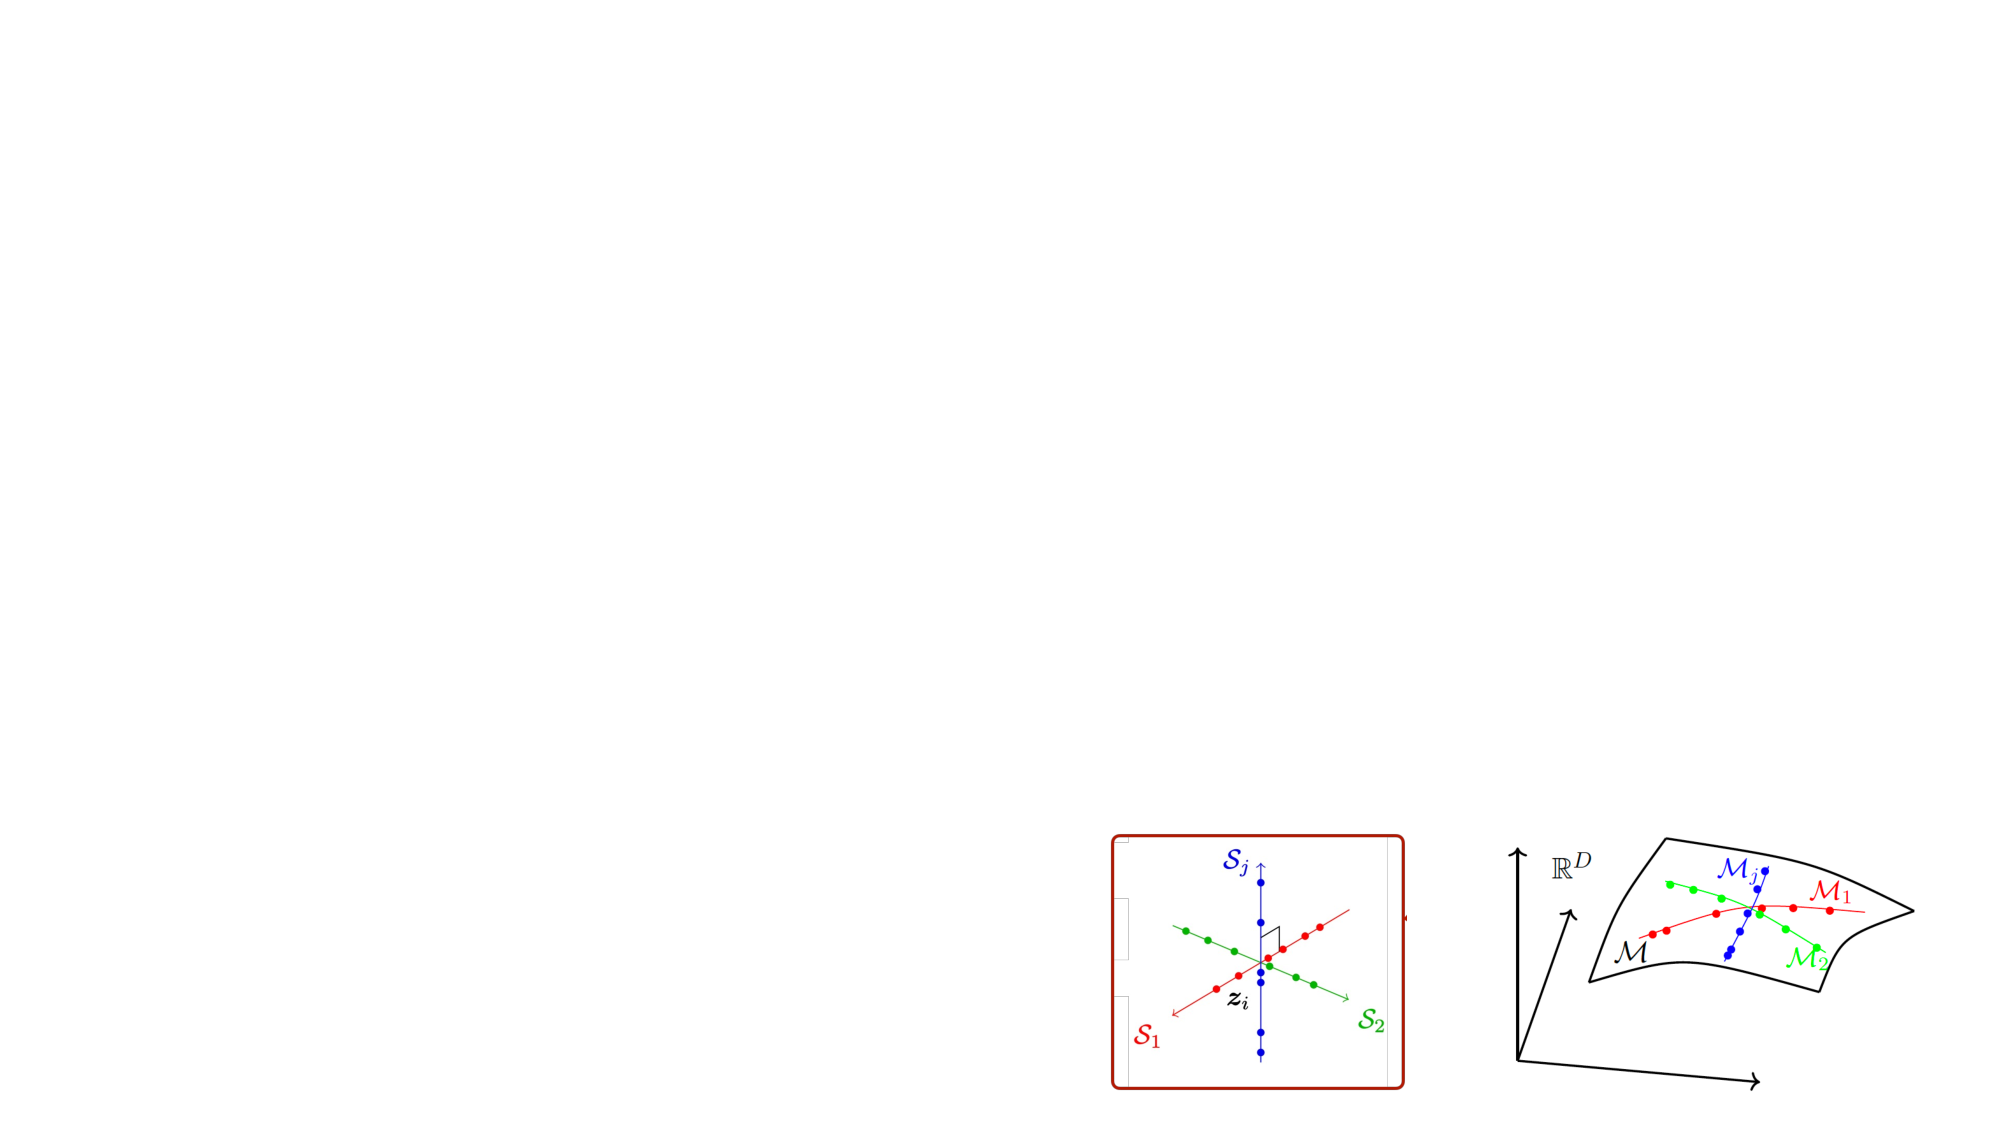
\includegraphics[width=0.8\linewidth]{\toplevelprefix/chapters/chapter1/figs/mixture.pdf}
    \caption{Data distributed on a mixture of (orthogonal) subspaces (left) or submanifolds (right).}
    \label{fig:mixture-models}
\end{figure}


\paragraph{Properties of Low-Dimensionality.}
Of course, temporal correlation in predictable sequences is not the only reason why data are low-dimensional. For example, the space of all images is humongous but most of the space consists of images that resemble structureless random images as shown in \Cref{fig:noise-image} left. Natural images and videos however are highly redundant because there is a strong spatial and temporal correlation among all pixel values. This is the reason why we can easily recognize whether an image is noisy or clean, as shown in \Cref{fig:noise-image} middle and right. Hence the distribution of natural images has a very low intrinsic dimension (relative to the total number of pixels of an image).

\begin{figure}
    \centering
    
\includegraphics[height=0.30\linewidth]{\toplevelprefix/chapters/chapter1/figs/Gaussian-noise.png}\hspace{2mm} 
    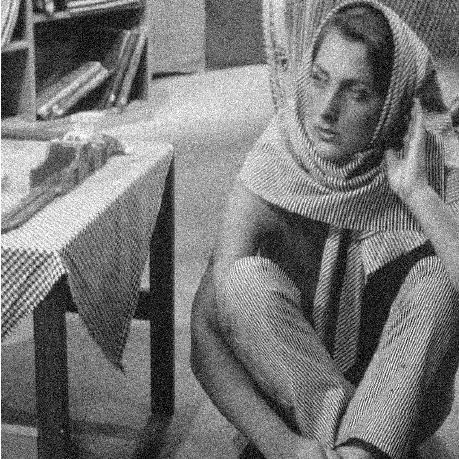
\includegraphics[height=0.30\linewidth]{\toplevelprefix/chapters/chapter1/figs/Standard-test-image-Barbara-of-size-512-512-pixels-including-Gaussian-noise-with.png} \hspace{2mm} 
    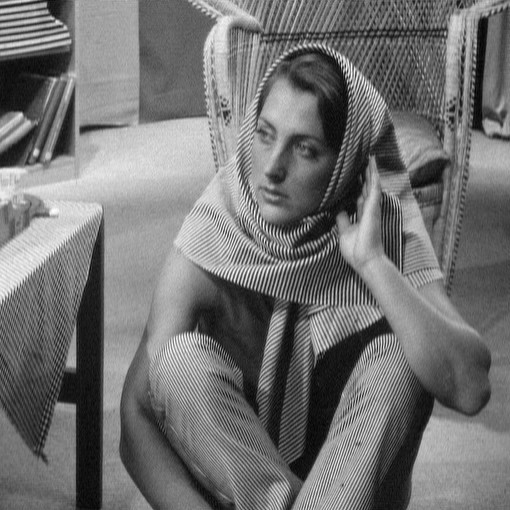
\includegraphics[height=0.30\linewidth]{\toplevelprefix/chapters/chapter1/figs/barbara.jpg}
    \caption{An image of random noise versus a noisy image and the original clean image. %\sdb{probably want to avoid using Lena given all the IEEE/PAMI-TC/etc.\ recent motions}
    }
    \label{fig:noise-image}
\end{figure}

Due to the importance and ubiquity of the task of  learning low-dimensional structures, the book {\em ``High-Dimensional Data Analysis with Low-Dimensional Models: Principles, Computation, and Applications''} \cite{Wright-Ma-2022} has stated in the beginning with a statement: ``{\em The problem of identifying the low-dimensional structure of signals or data in high-dimensional
spaces is one of the most fundamental problems that, through a long
history, interweaves many engineering and mathematical fields such as system
theory, signal processing, pattern recognition, machine learning, and statistics.}''

Note that by enforcing the observed data point $\vx$ to be on a low-dimensional surface, we essentially have made the entries of $\vx$ very dependent on each other and in some sense have made the entries very ``predictable'' from values of other entries. For example, if we know that the data are constrained on a $d$-dimensional surface in $\R^d$, then it allows us to do many useful things with the data besides prediction: %\yima{Maybe some illustrations for these properties.}
\begin{itemize}
    \item \textbf{completion}: in general, given more than $d$ entries of a typical sample $\vx$, the rest of its entries usually can be {\em uniquely} determined.\footnote{Prediction becomes a special case of this property.} 
    \item \textbf{denoising}: suppose entries of a sample $\vx$ are perturbed by {\em small} noises, they can be effectively removed by projecting $\vx$ back onto the surface.
    \item \textbf{error correction}: suppose a small number of {\em unknown} entries of $\vx$ are arbitrarily corrupted, they can be effectively and efficiently corrected. 
\end{itemize}
Figure \ref{fig:low-dim-properties} illustrates these properties with a low-dimensional linear structure: a one-dimensional line in a two-dimensional plane. 

\begin{figure}
    \centering
    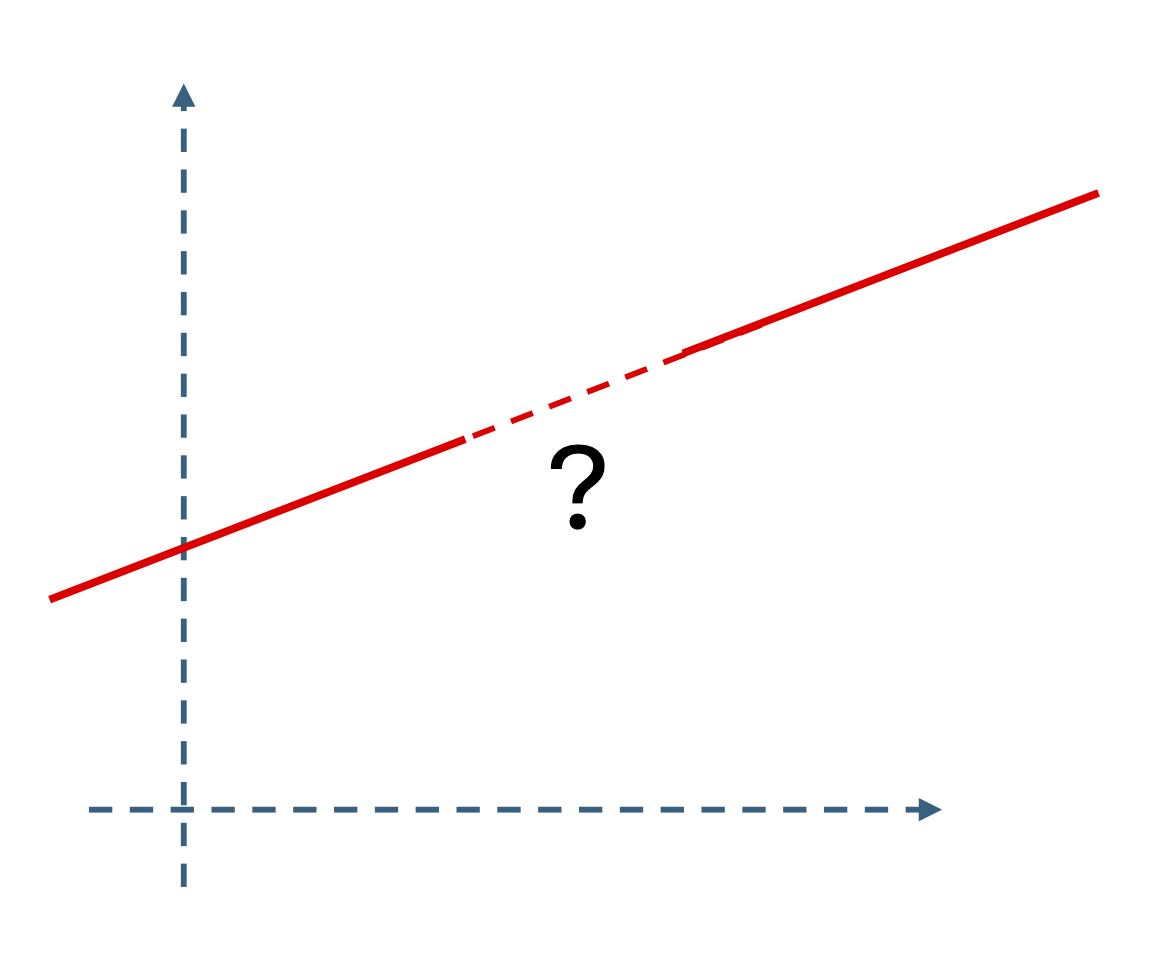
\includegraphics[height=0.28\linewidth]{\toplevelprefix/chapters/chapter1/figs/Completion-low-dim.png}     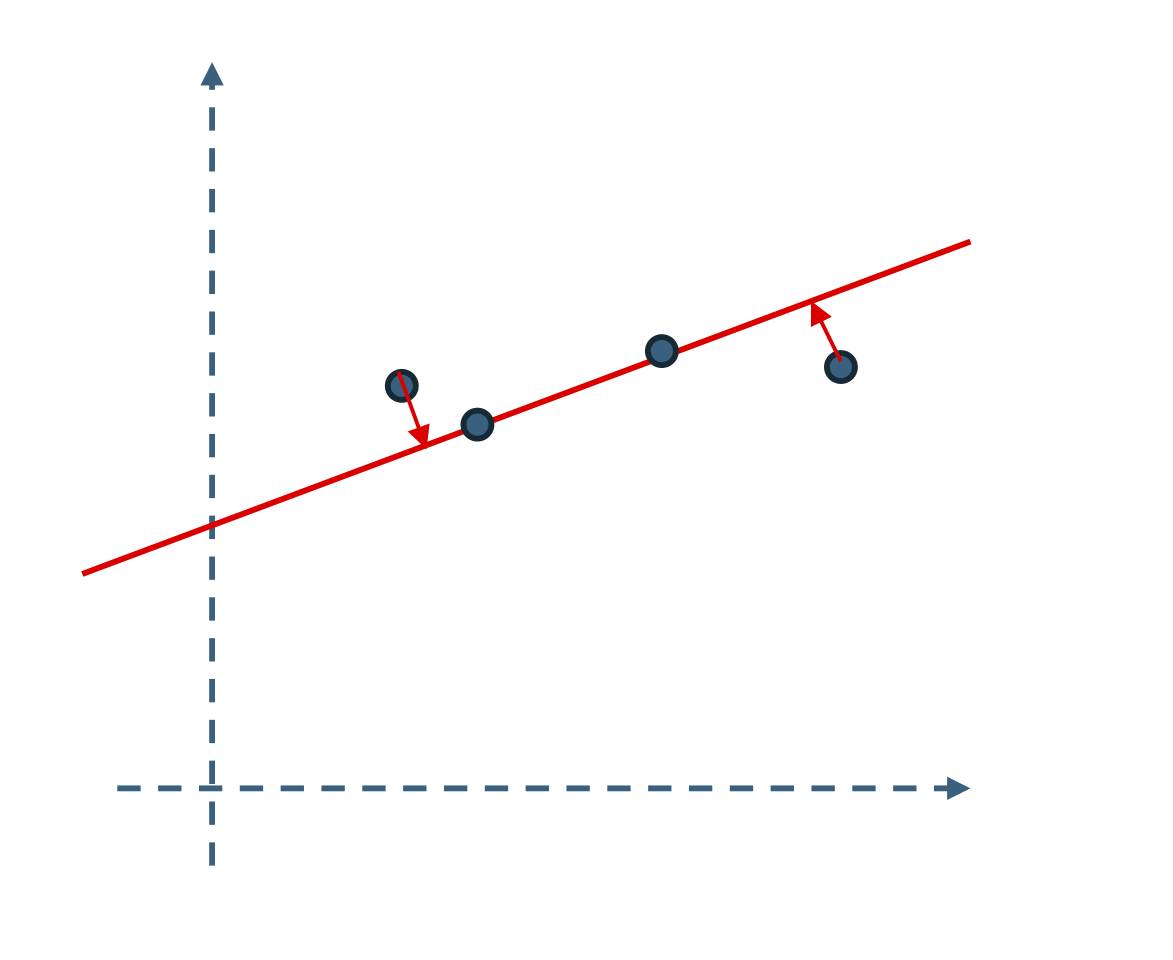
\includegraphics[height=0.28\linewidth]{\toplevelprefix/chapters/chapter1/figs/Denoising-low-dim.png} 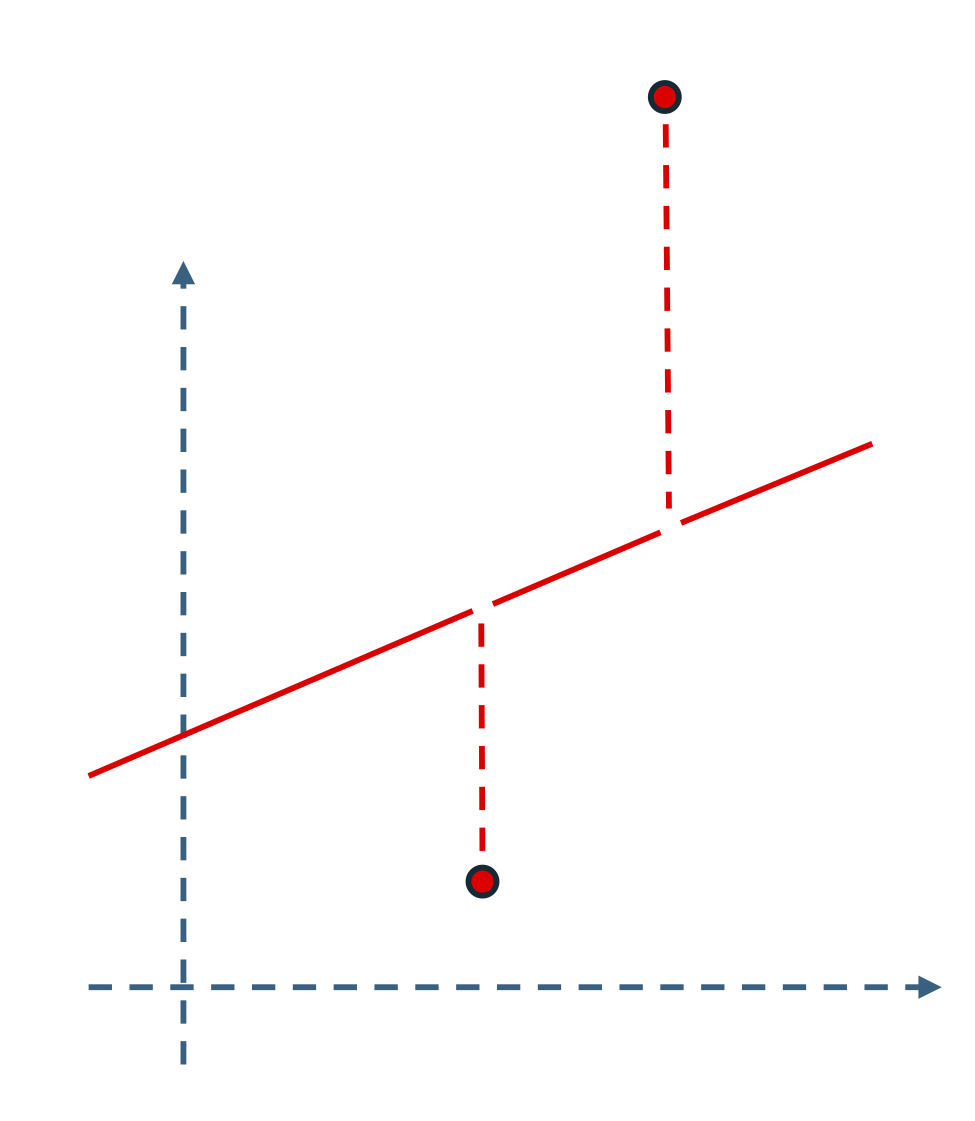
\includegraphics[height=0.32\linewidth]{\toplevelprefix/chapters/chapter1/figs/Correction-low-dim.png} 
    \caption{Illustration of properties of a low-dimensional (linear) structure: it enables completion (left), denoising (middle), and error correction (right).}
    \label{fig:low-dim-properties}
\end{figure}

In fact, under mild conditions, the above properties are generalizable to many other low-dimensional structures in high-dimensional spaces \cite{Wright-Ma-2022}. Interestingly, as we will see in this book, these useful properties such as completion and denoising will inspire effective methods to learn such low-dimensional structures. 

In the above, for simplicity, we have only used the deterministic case to introduce the important notion of predictability and low-dimensionality. Hence, the data (or sampled segments) precisely lie on some geometric structures such as subspaces or surfaces. In practice, as we have alluded to before, there is always a certain level of uncertainty or randomness in the data. In this case, we may assume that the data have a probability distribution, with a probability density function $p(\vx)$. We say that a distribution is ``low-dimensional'' if its density concentrates around a geometric structure that is rather low-dimensional, say a subspace, a surface or a mixture of them, as shown in Figure \ref{fig:mixture-models}. Notice that, from a practical point of view, such a density function $p(\x)$, once learned, can serve as a very powerful prior for estimating $\x$ based on partial, noising, or corrupted observation, say: 
\begin{equation}
\y = f(\x) + \boldsymbol{n},
\end{equation}
by computing the conditional estimation $\hat{\x}(\y) = \mathbb{E}(\x \mid \y)$ or through sampling the conditional distribution $\hat{\x}(\y) \sim p(\x\mid \y)$.\footnote{Modern generative AI technologies such as (conditioned) image generation very much rely on this fact, as we will elaborate on in Chapter \ref{ch:conditional-inference}.}

Our discussions above have led to the main thesis of this book: {\em any learning methods or intelligent systems should and could rely on is that the world is predictable hence the distribution of the observed data samples have low-dimensional supports.} The remaining question is how to learn such low-dimensional structures correctly, via effective and efficient computable means. 

\section{How to Learn?}


\subsection{Analytical Approaches}
\label{sec:analytical}
%\paragraph{Analytical models for low-dimensionality.}
Note even if a predictive function is tractable to compute, it does not imply it is tractable or scalable to learn this function from a number of sampled segments. Of course, one classical approach to ensure the problems are tractable or amenable to efficient solutions is to make explicit assumptions about the family of low-dimensional structures we are dealing with. Historically, due to limited computation and data, simple and idealistic analytical models were always the first to be studied as they often offer efficient closed-form or numerical solutions. In addition, they can provide insights to the more general problems and they often already provide useful solutions to important though limited cases. In old days when computational resource was scarce, analytical models that permitted efficient closed-form or numerical solutions were the only cases that could be implemented. {\em Linear structures} became the first classes of models to be thoroughly studied.

For example, arguably the simplest case is to assume the data is distributed around a single low-dimensional subspace in a high-dimensional space. Or somewhat equivalently, one may assume the data is distributed according to an almost degenerate low-dimensional Gaussian. Identifying such a subspace or Gaussian from a finite number of (noisy) samples is then the classical problem of principal component analysis (PCA) and  effective algorithms have been developed for this class of models \cite{JolliffeI2002}. One can make the family of models increasingly more complex and expressive. For instance, one may assume the data are distributed around a certain mixture of low-dimensional components (subspaces or low-dimensional Gaussians), as in the case of independent component analysis (ICA) \cite{Ans-1985}, dictionary learning (DL), generalized principal component analysis (GPCA) \cite{Vidal-GPCA}, or the even more general class of sparse low-dimensional models that have been studied extensively in recent years in fields such as compressive sensing \cite{Wright-Ma-2022}. 

Around all these analytical model families, the central problem of study is always how to identify {\em the most compact} model within each family that best fits the given data. Below, we give a very brief account of these classical analytical models but leave a more systematic study to Chapter \ref{ch:classic}. In theory, these analytical models have provided us with tremendous insights into the geometric and statistical properties of low-dimensional structures. They often give us closed-form solutions or efficient and scalable algorithms which are very useful for data whose distributions can be well approximated by such models. More importantly, for more general problems, they provide us with a general sense of how easy or difficult the problem of identifying low-dimensional structures can be, and what the basic ideas are to approach such a problem.



%Hence, in this book, we choose to introduce and study these somewhat idealistic structures first in Chapter \ref{ch:classic}, not only because we can derive efficient solutions for them with rigorous theoretical guarantees, but also the basic ideas of their solutions carry over to the more general (nonlinear) structures and distributions that we will study in later chapters. 

\subsubsection{Linear Dynamical Systems}
\label{sec:linear-systems}

\paragraph{Wiener Filter.}

As we have discussed before in Section \ref{sec:predictability}, a main task of intelligence is to learn what is predictable in sequences of observations. Probably the simplest class  of predictable sequences, or signals, are generated via a {\em linear time-invariant} (LTI) process:
\begin{equation}
    x[n] = h[n]*z[n] + \epsilon[n], 
    \label{eqn:Wiener-model}
\end{equation}
where $z$ is the input and $h$ is the impulse response function.\footnote{Normally $h$ is assumed to have certain nice structures, say finite length or banded spectrum.}  Here $\epsilon[n]$ is some additive noise in the observations. The problem is that given the input process  $\{z[n]\}$ and observations of the output process $\{x[n]\}$, how to find the optimal $h[n]$ such that $\hat x[n] = h[n]*z[n]$ predicts $x[n]$ is an optimal way. In general, we measure the goodness of the prediction by the minimum mean squared error (MMSE):
\begin{equation}
    \min_{h} \mathbb{E} \big[\epsilon[n]^2\big] = \mathbb{E} \big[\|x[n] - h[n]*z[n]\|_2^2\big].
\end{equation}
The optimal solution $h[n]$ is referred to as a (denoising) filter. Norbert Wiener, the same person initiated the Cybernetics movement, studied this problem in 1940s and gave an elegant closed-form  solution known as the {\em Wiener filter} \cite{Wiener-1942,Wiener-1949}. This became one of the most fundamental results in the field of  Signal Processing.

\paragraph{Kalman Filter.} 
The idea of denoising or filtering for a dynamic process was later extended to a linear time-invariant system described by a (finite-dimensional) state-space model by Rudolph Kalman in the 1960s:
\begin{equation}
    \z[n] = \boldsymbol{A} \z[n-1] + \boldsymbol{B}\boldsymbol{u}[n] + \boldsymbol{\epsilon}[n]. 
    \label{eqn:linear-state-space}
\end{equation}
The problem is how we can estimate the state of the system $\z[n]$ from noisy observations of the form: \begin{equation}\x[n] = \boldsymbol{C} \z[n] + \boldsymbol{w}[n],
\label{eqn:Kalman-model}
\end{equation}
where $\boldsymbol{w}$ is some (white) noise. The optimal causal\footnote{Which means the estimation can only use observations up to the current  time step $n$. Kalman filter is always causal whereas Wiener filter needs not to be.} state  estimator that minimizes the MMSE-type prediction error
\begin{equation}
    \min \mathbb{E}\big[ \|\x[n] - \boldsymbol{C}\z[n]\|_2^2\big]
\end{equation}
is given in closed-form by the so-called {\em Kalman filter} \cite{kalman1960new}. This is one of the corner stones of modern Control Theory because it allows us to estimate the state of a dynamical system from its noisy observations. Then one can subsequently introduce a (linear) state feedback, say of the form $\boldsymbol{u}[n] = \boldsymbol{F} \hat{\boldsymbol{z}}[n]$, and make the closed-loop system fully autonomous, as we saw in equation \eqref{eqn:recursive-closed-loop}. 

\paragraph{Identification of Linear Dynamical Systems.}
To derive the Kalman filter, the system parameters $(\boldsymbol{A}, \boldsymbol{B}, \boldsymbol{C})$ are assumed to be known. If they are not given in advance, it would be a more challenging problem known as {\em system identification}: how to {\em learn} the parameters $(\boldsymbol{A}, \boldsymbol{B}, \boldsymbol{C})$ from (many samples of) the input sequence $\{\boldsymbol{u}[n]\}$ and observation sequence $\{\x[n]\}$. This is a classic problem in systems theory. If the system is linear, it can be shown that the input and output sequences $\{\boldsymbol{u}[n], \x[n]\}$ would jointly lie on certain low-dimensional subspace\footnote{which has the same dimension as the order of the state-space model \eqref{eqn:linear-state-space}. }. Hence the identification problem is essentially equivalent to identifying this low-dimensional subspace \cite{OverscheeP1996,Liu-2009-CDC,Liu-2010-SIAM}. 

Note that the above problems have two things in common: first, the (noise-free)  sequences or signals are assumed to be generated by an explicit family of parametric models; second, these models essentially are all linear. So conceptually, let $\x_o$ be a random variable whose ``true'' distribution is supported on a low-dimensional linear subspace, say $S$. To a large extent, Wiener filter and Kalman filter all try to estimate such an $\x_o$ from its noisy observations:
\begin{equation}
    \x = \x_o + \boldsymbol{\epsilon}, \quad \x_o \sim S, 
\end{equation}
where $\boldsymbol{\epsilon}$ is typically a random Gaussian noise (or process). Hence, essentially, their solutions all rely on identifying a low-dimensional linear subspace that best fits the observed (noisy) data. Then by projecting the data onto this subspace, one obtains the optimal denoising operations, all in closed form.   

%Parallel developments in systems theory, signal/image processing, statistical learning, and machine learning: How to effectively and efficiently learn a more general low-dimensional distribution in a high-dimensional space? The history of denoising (Wiener filter and Kalman filter) for linear  systems. Empirical 

\subsubsection{Linear and Mixed Linear Models}
\label{sec:PCA-ICA}
\paragraph{Principal Component Analysis.}
From the above problems in classical signal processing and system identification, we see that the main task behind of all these problems is to learn from noisy observations a {\em single} low-dimensional linear subspace. Mathematically, we may model such a structure as:
\begin{equation}
    \x = \boldsymbol{u}_1 z_1 + \boldsymbol{u}_2 z_2 + \cdots + \boldsymbol{u}_d z_d + \boldsymbol{\epsilon} =  \boldsymbol{U} \z + \boldsymbol{\epsilon}, \quad \boldsymbol{U} \in \mathbb{R}^{D\times d}
    \label{eqn:PCA-model}
\end{equation}
where $\boldsymbol{\epsilon} \in \mathbb{R}^D$ is some small random noise. Figure \ref{fig:PCA} illustrates such a distribution with two principal components.
\begin{figure}
    \centering
    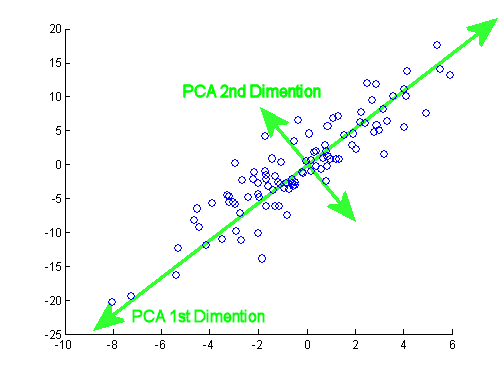
\includegraphics[width=0.5\linewidth]{\toplevelprefix/chapters/chapter1/figs/PCA.png}
    \caption{A distribution with two principal components.}
    \label{fig:PCA}
\end{figure}
The problem is to find the subspace basis $\boldsymbol{U}$ from many samples of $\x$. A typical approach to estimate the subspace $\boldsymbol{U}$ is to minimize the variance of the noise, also known as the minimum mean square error (MMSE):
\begin{equation}
    \min_{\boldsymbol{U}} \mathbb{E}\big[\|\boldsymbol{\epsilon}\|_2^2\big] = \mathbb{E}\big[\|\x - \boldsymbol{U} \z\|_2^2\big].
\end{equation}
Notice that this is essentially a denoising task: once the basis $\boldsymbol{U}$ is correctly found, we can denoise the noisy sample $\x$ by projecting it onto the low-dimensional subspace spanned by $\boldsymbol{U}$ as 
\begin{equation}
\x \rightarrow \hat \x = \boldsymbol{U}\boldsymbol{U}^\top \x. 
\end{equation}
If the noise is small and if we learned the correct low-dimensional subspace $\boldsymbol{U}$, we should expect $\x \approx \hat \x$. That is, PCA is a special case of the auto-encoding:
\begin{equation}
    \x   \xrightarrow{\hspace{2mm} \boldsymbol{U}^\top\hspace{2mm}} \z  \xrightarrow{\hspace{2mm} \boldsymbol{U} \hspace{2mm}} \hat \x.
       \label{eqn:auto-encoding-PCA}
\end{equation}
Only here because of the simple data structure, the encoder $\mathcal{E}$ and decoder $\mathcal{D}$ both become simple linear operators ((projecting and lifting).

This is a classic problem in statistics known as the Principal Component Analysis (PCA). It was first studied by Pearson in 1901 \cite{Pearson1901} and later independently by Hotelling in 1933 \cite{Hotelling1933}. This topic is systematically summarized in the classic book \cite{Jolliffe1986,JolliffeI2002}.
In addition, one may explicitly assume the data $\x$ is distributed according to a single low-dimensional Gaussian:
\begin{equation}
    \x \sim \mathcal{N}(\boldsymbol{0}, \boldsymbol{U}\boldsymbol{U}^\top + \sigma \I), \quad \boldsymbol{U} \in \mathbb{R}^{D\times d},
\end{equation}
which is equivalent to assuming that  $\z$ in the above PCA model \eqref{eqn:PCA-model} is a standard normal distribution. 
This is known as Probabilistic PCA \cite{TippingM1999}. 

In this book, we will revisit  PCA in Chapter \ref{ch:classic}, from the perspective of learning a low-dimensional distribution. Our goal is to use this simple and idealistic model to convey some of the most fundamental ideas for learning a compact representation for a low-dimensional distribution, including the important notion of compression via denoising and autoencoding for a consistent representation.

\paragraph{Independent Component Analysis.}
Independent component analysis (ICA) was originally proposed by \cite{Ans-1985} as a classic model for {\em learning a good representation}. In fact it was originally proposed as a simple mathematical model for our memory. The ICA model takes a deceivingly similar form as the above PCA model \eqref{eqn:PCA-model} by assuming that the observed random variable $\x$ is a linear superposition of multiple independent components $z_i$:
\begin{equation}
    \x = \boldsymbol{u}_1 z_1 + \boldsymbol{u}_2 z_2 + \cdots + \boldsymbol{u}_d z_d  + \boldsymbol{\epsilon} =  \boldsymbol{U} \z + \boldsymbol{\epsilon}.
    \label{eqn:ICA-model}
\end{equation}
However, here the components $z_i$ are assumed to be independent {\em non-Gaussian} variables. For example, a popular choice is
\begin{equation}
    z_i = \sigma_i \cdot w_i, \quad \sigma_i \sim B(1,p),
    \label{eqn:ICA-modes}
\end{equation}
where $\sigma_i$ is a Bernoulli random variable and $w_i$ could be a constant value or another random variable, say Gaussian.\footnote{Even if $w$ is Gaussian, $\sigma w$ is no longer a Gaussian variable!}  The ICA problem is trying to identify both $\boldsymbol{U}$ and $\z$ from observed samples of $\x$. Figure \ref{fig:ICA-PCA} illustrates the difference between ICA and PCA.

\begin{figure}
    \centering
    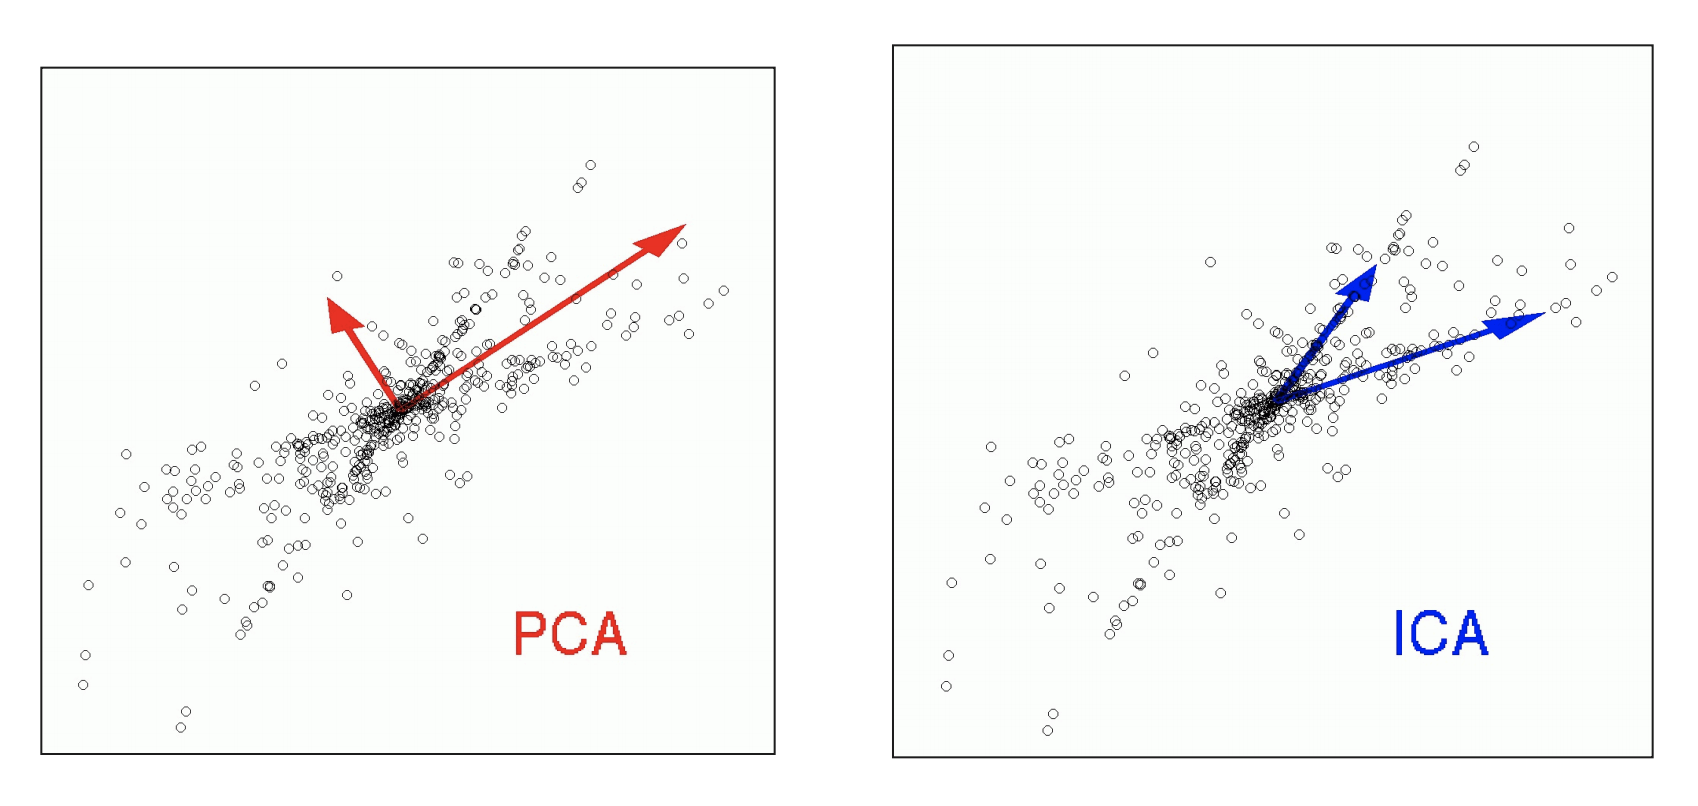
\includegraphics[width=0.7\linewidth]{\toplevelprefix/chapters/chapter1/figs/PCA_ICA.png}
    \caption{PCA (left) versus ICA (right).}
    \label{fig:ICA-PCA}
\end{figure}

Although the (decoding) mapping from $\z$ to $\x$ seems linear and easy once $\boldsymbol{U}$ and $\z$ are learned, the (encoding) mapping from $\x$ to $\z$ can be complicated and may not be represented by a simple linear mapping. Hence ICA generally gives an autoencoding of the form:
\begin{equation}
    \x   \xrightarrow{\hspace{2mm} \mathcal{E}\hspace{2mm}} \z  \xrightarrow{\hspace{2mm} \boldsymbol{U} \hspace{2mm}} \hat \x.
       \label{eqn:auto-encoding-ICA}
\end{equation}
Hence, unlike PCA, ICA is a little more difficult to analyze and solve. In 1990s, folks like Erkki Oja and Aapo Hyv\"{a}rinen \cite{hyvarinen-1997,Hyvrinen-2000} have made significant theoretical and algorithmic contributions to ICA. In Chapter \ref{ch:classic}, we will study and give a solution to ICA from which the encoding mapping $\mathcal{E}$ will become clear.



\paragraph{Sparse Structures and Compressive Sensing.}
As one may see, if $p$ in \eqref{eqn:ICA-modes} is very small, the probability that any of the components is non-zero is small. In this case, we say $\x$ is sparsely generated and it concentrates on a set of linear subspaces of dimension $k = p \cdot d$. Hence, to some extent, we may extend the above ICA model to a more general family of low-dimensional structures known as sparse models. 

A $k$-sparse model is defined to be consisting of the set of all {\em $k$-sparse vectors}:
\begin{equation}
    \mathcal{Z} = \{\z \in \mathbb{R}^n \mid \|\z\|_0 \le k\},
\end{equation}
where $\| \cdot \|_0$ is the $\ell^0$-norm that counts the number of non-zero entries in a vector $\z$. That is, $\mathcal{Z}$ is the union of all $k$-dimensional subspaces that align with the coordinate axes, as illustrated in Figure \ref{fig:mixture-models} left. One important problem in classic signal processing and statistics is how to recover a sparse vector $\z$ from its linear observations:
\begin{equation}
    \x = \boldsymbol{A} \z + \boldsymbol{\epsilon}, \quad \boldsymbol{A} \in \mathbb{R}^{m\times n}
    \label{eqn:sparse-model}
\end{equation}
where $\boldsymbol{A}$ is given but typically $m < n$ and $\boldsymbol{\epsilon}$ is some small noise. This seemingly benign problem turns out to be NP-hard to compute and it is even hard to approximate (see the book \cite{Wright-Ma-2022} for details). 

So despite a very rich and long history of study which can be dated back as early as  the 18th century \cite{Boscovichca1750}, there was no provably efficient algorithm to solve this class of problems, although many heuristic algorithms have been proposed and developed between the 1960s and the 1990s. Some are rather effective in practice but without any rigorous justification. A major breakthrough came in the early 2000s when a few renowned mathematicians including David Donoho, Emmanuel Cand\`{e}s, and Terence Tao \cite{donoho2005neighborly,Candes2005,CandesE2005-IT} established a rigorous theoretical framework that allows us to characterize  precise conditions under which the sparse recovery problem can be solved effectively and efficient, say via a convex $\ell^1$ minimization:
\begin{equation}
    \min \|\z\|_1 \quad \mbox{subject to} \quad \| \x - \boldsymbol{A}\z\|_2 \le \epsilon,
\end{equation}
where $\|\cdot \|_1$ is the sparsity-promoting $\ell^1$ norm of a vector and $\epsilon$ is some small constant. Any solution to this problem essentially gives a sparse coding mapping:
\begin{equation}
    \x   \xrightarrow{\hspace{2mm} \mathcal{E} \hspace{2mm}}  \z.
       \label{eqn:decoding-sparse}
\end{equation}
We will give a brief account of such an algorithm, hence mapping, in Chapter \ref{ch:classic} which will reveal interesting fundamental connections between sparse coding and deep learning.\footnote{Although similarities between algorithms for sparse coding and deep networks were noticed as early as in 2010 \cite{gregor2010learning}.}

As it turns out, conditions under which $\ell^1$ minimization succeeds are surprisingly general. The minimum number of measurements $m$ required for a successful recovery is only proportional to the intrinsic dimension of the data $k$. This is now known as the {\em compressive sensing} phenomenon \cite{CandesE2006-ICM}. Moreover, this phenomenon is not unique to sparse structures. It also applies to very broad families of low-dimensional structures such as low-rank matrices etc. These results have fundamentally changed our understanding about recovering low-dimensional structures in high-dimensional spaces. This dramatic reverse of fortune with high-dimensional data analysis was even celebrated as the {\em ``blessing of dimensionality''} by David Donoho \cite{DonohoD2000} as opposed to the typical pessimistic belief in  ``curse of dimensionality'' for high-dimensional problems. This coherent and complete body of results has  been systematically organized in the book \cite{Wright-Ma-2022}. 

From a computational perspective, one cannot over-estimate the significance of this new framework. It has fundamentally changed our views about an important class of problems previously believed to be largely intractable. It has enabled us to develop extremely efficient algorithms that scale gracefully with the dimension of the problem, hence making the problem of sparse recovery from:
\begin{equation}
    \mbox{\textbf{intractable}} \;
   \Longrightarrow \; \mbox{\textbf{tractable}} \; \Longrightarrow \; 
   \mbox{\textbf{scalable}}.
\end{equation}
These algorithms also come with rigorous theoretical guarantees of their correctness given precise requirements in data and computation. The rigorous and precise nature of this approach is almost opposite to that of practicing deep neural networks, which is largely empirical. Yet, despite their seemingly opposite styles and standards, we now know both approaches share a common goal: {\em trying to pursue low-dimensional structures in high-dimensional spaces.}

\paragraph{Dictionary Learning.}
Conceptually, an even harder problem than the sparse coding problem \eqref{eqn:sparse-model} is when the observation matrix $\boldsymbol{A}$ is not even known in advance and we need to learn $\boldsymbol{A}$ from a set of (possibly noisy) observations, say $\X = [\x_1, \x_2, \ldots, \x_n]$:
\begin{equation}
    \X = \boldsymbol{A} \Z + \boldsymbol{E}, \quad \boldsymbol{A} \in \mathbb{R}^{m\times n}.
    \label{eqn:dictionary-learning}
\end{equation}
Here we are given only $\X$ but not the corresponding $\Z = [\z_1, \z_2, \ldots, \z_n]$ nor the noise term $\boldsymbol{E}= [\boldsymbol{\epsilon}_1, \boldsymbol{\epsilon}_2, \ldots, \boldsymbol{\epsilon}_n]$, except for knowing $\z_i$'s are sparse. This is known as the {\em dictionary learning} problem, which can be viewed as a generalization to the ICA problem \eqref{eqn:ICA-model} discussed earlier. In other words, given the distribution of the data $\X$ to be the image of a standard sparse distribution $\Z$ under a linear transform $\boldsymbol{A}$, we like to learn $\boldsymbol{A}$ and its ``inverse'' mapping $\mathcal{E}$ such that we obtain an autoencoder:
\begin{equation}
    \X   \xrightarrow{\hspace{2mm} \mathcal{E} \hspace{2mm}}  \Z \xrightarrow{\hspace{2mm} \boldsymbol{A} \hspace{2mm}} \X?
       \label{eqn:decoding-DL}
\end{equation}

One can see what is in common with PCA, ICA, and Dictionary Learning is that they all assume that the distribution of the data is supported around low-dimensional linear or mixed linear structures. They all require to learn a (global or local) basis of the linear structures, from probably noisy samples of the distribution. In Chapter \ref{ch:classic}, we will study how to identify low-dimensional structures through these classical models. In particular, we will see an interesting and important fact: all these low-dimensional (piecewise) linear models can be learned effectively and efficiently by the same type of fast algorithms, known as {\em power iteration} \cite{Zhai-2020}. Although the above linear or mixed linear models are somewhat too simplistic or idealistic for most real-world data, understanding these models is an important first step toward understanding more general low-dimensional distributions. 

\subsubsection{General Distributions}\label{sec:denoising-intro}

The distributions of real-world data such as images, videos, and audio are too complex to be modeled by above, somewhat idealistic, linear models or Gaussian processes. We normally do not know {\em a priori} they are generated from which family of parametric models.\footnote{Although in history there had been many attempts to develop analytical models for these data, such as random fields or stochastic processes for imagery data \cite{Mumford-1999}, as we have discussed in the previous section.} In practice, we typically only have many samples from their distributions -- the empirical distributions. Obviously, in such cases, we normally cannot expect to have any closed-form solutions for their low-dimensional structures, nor for the resulting denoising operators.\footnote{Unlike the cases of PCA, Wiener filter, and Kalman filter.} So we need to develop a more general solution to these empirical distributions, not necessarily in closed form but at least efficiently computable. If we did this correctly, solutions to the aforementioned linear models should become their special cases. 

\paragraph{Denoising.} In the 1950s, statisticians became interested in the problem of denoising data drawn from an arbitrary distribution. Let $\x_o$ be a random variable with probability density function $p_o(\cdot)$. So if we observe a noisy version of $\x_o$:
\begin{equation}
    \x = \x_o + \sigma \vg, 
\end{equation}
where $\vg \sim \dNorm(\vzero, \vI)$ is standard Gaussian noise and $\sigma$ is the noise level of the observation. Let $p(\cdot)$ be the probability density function of $\x$,\footnote{That is, $p(\x) = \int_{-\infty}^{\infty} \phi_{\sigma}(\x - \z)p_o(\z) \odif{\z}$, where $\phi_{\sigma}$ is the density function of the Gaussian distribution $\mathcal{N}(\boldsymbol{0}, \sigma^2 \boldsymbol{I})$.} Amazingly, the posterior expectation of $\x_o$ given $\x$ can be calculated by an elegant formula, known as the Tweedie's formula \cite{Robbins1956AnEB}:\footnote{Herbert Robbins gave the credits of this formula to Maurice Kenneth Tweedie from their personal correspondence.}
\begin{equation}
    \hat \x_o = \mathbb{E}[\x_o\mid \x] = \x + \sigma^2 \nabla \log p(\x).
\end{equation}
As can be seen, from the formula, the function $\nabla \log p(\x)$ plays a very special role in denoising the observation $\x$ here. The noise $\vg$ can be explicitly estimated as
\begin{equation}
    \hat{\vg} = \frac{\x - \hat \x_o}{\sigma} = -\sigma \nabla \log p(\x),
\end{equation}
for which we only need to know the distribution $p(\cdot)$ of $\x$ not the ground truth $p_o(\cdot)$ for $\x_o$. An important implication of this result is that if we add Gaussian noise to any distribution, the denoising process can be done easily if we can somehow get hold of the function $\nabla \log p(\x)$.

Because this is such an important and useful result, it has been rediscovered and used in many different contexts and areas. For example, after Tweedie's formula \cite{Robbins1956AnEB}, it was rediscovered a few years later by \cite{Miyasawa61}. In the early 2000s, the function $\nabla \log p(\x)$ was rediscovered again in the context of learning a general distribution and was named the ``score function'' by Aapo Hyv\"{a}rinen \cite{hyvarinen05a}. But its connection to (empirical Bayesian) denoising was soon recognized by \cite{Vincent2011}.
Generalizations to other measurement distributions (beyond Gaussian noise) have been made by Eero Simoncelli's group \cite{Raphan10}, and later applied to image denoising \cite{Kadkhodaie21a,ho2020denoising}.

\begin{figure}
    \centering
    %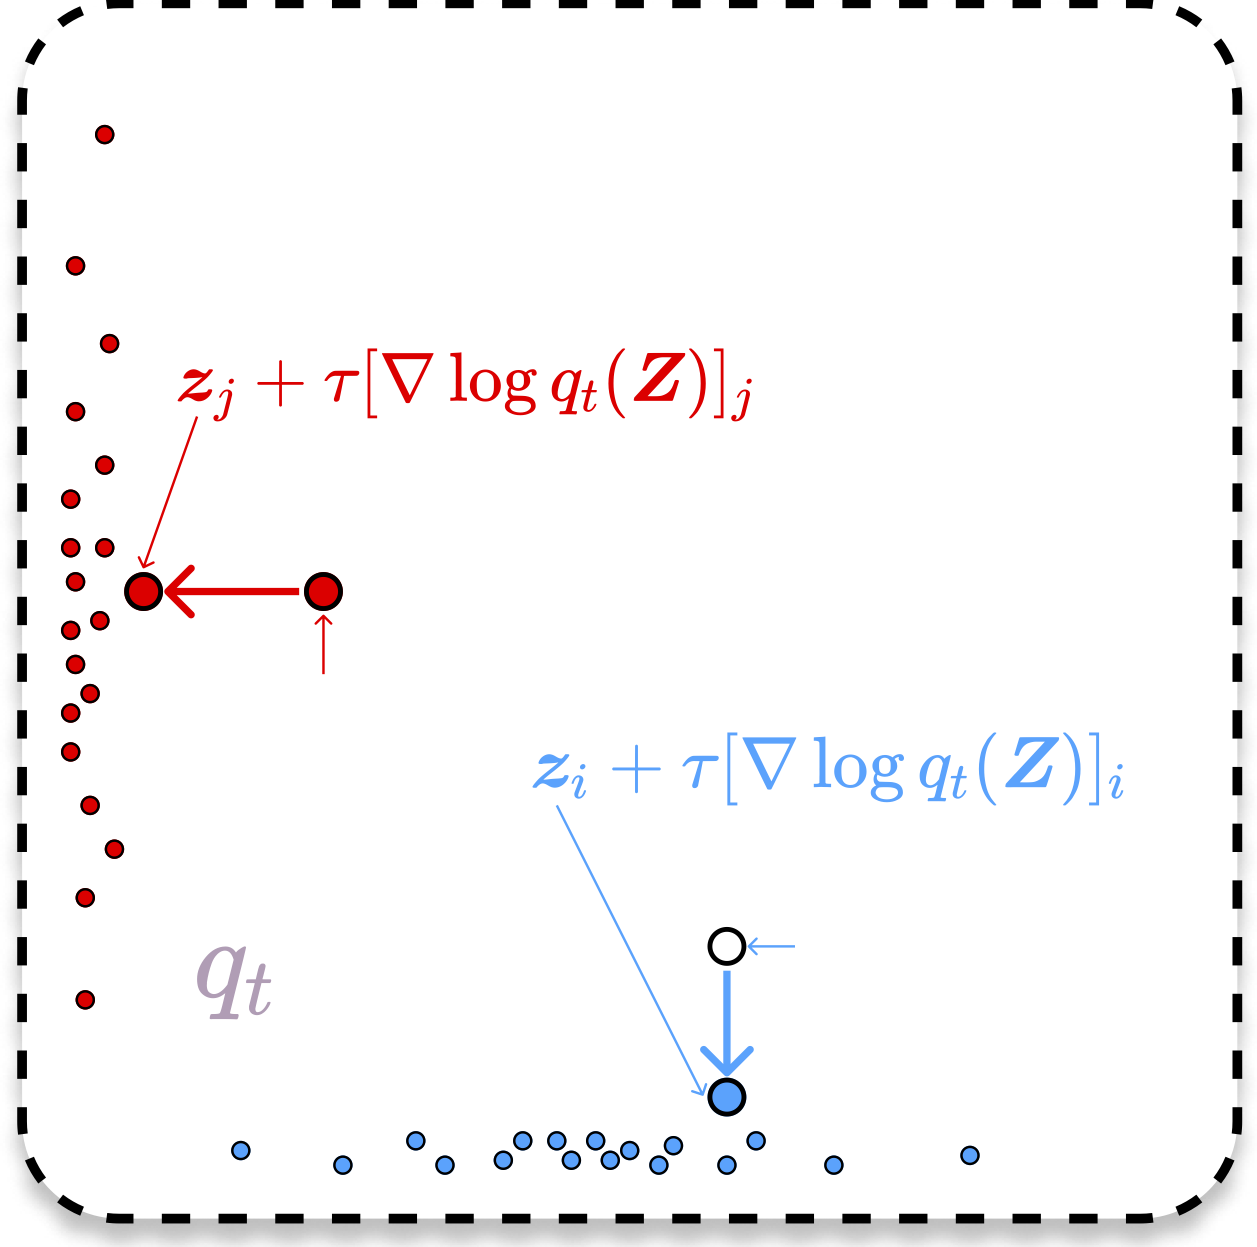
\includegraphics[width=0.45\linewidth]{\toplevelprefix/chapters/chapter1/figs/Score.png}
    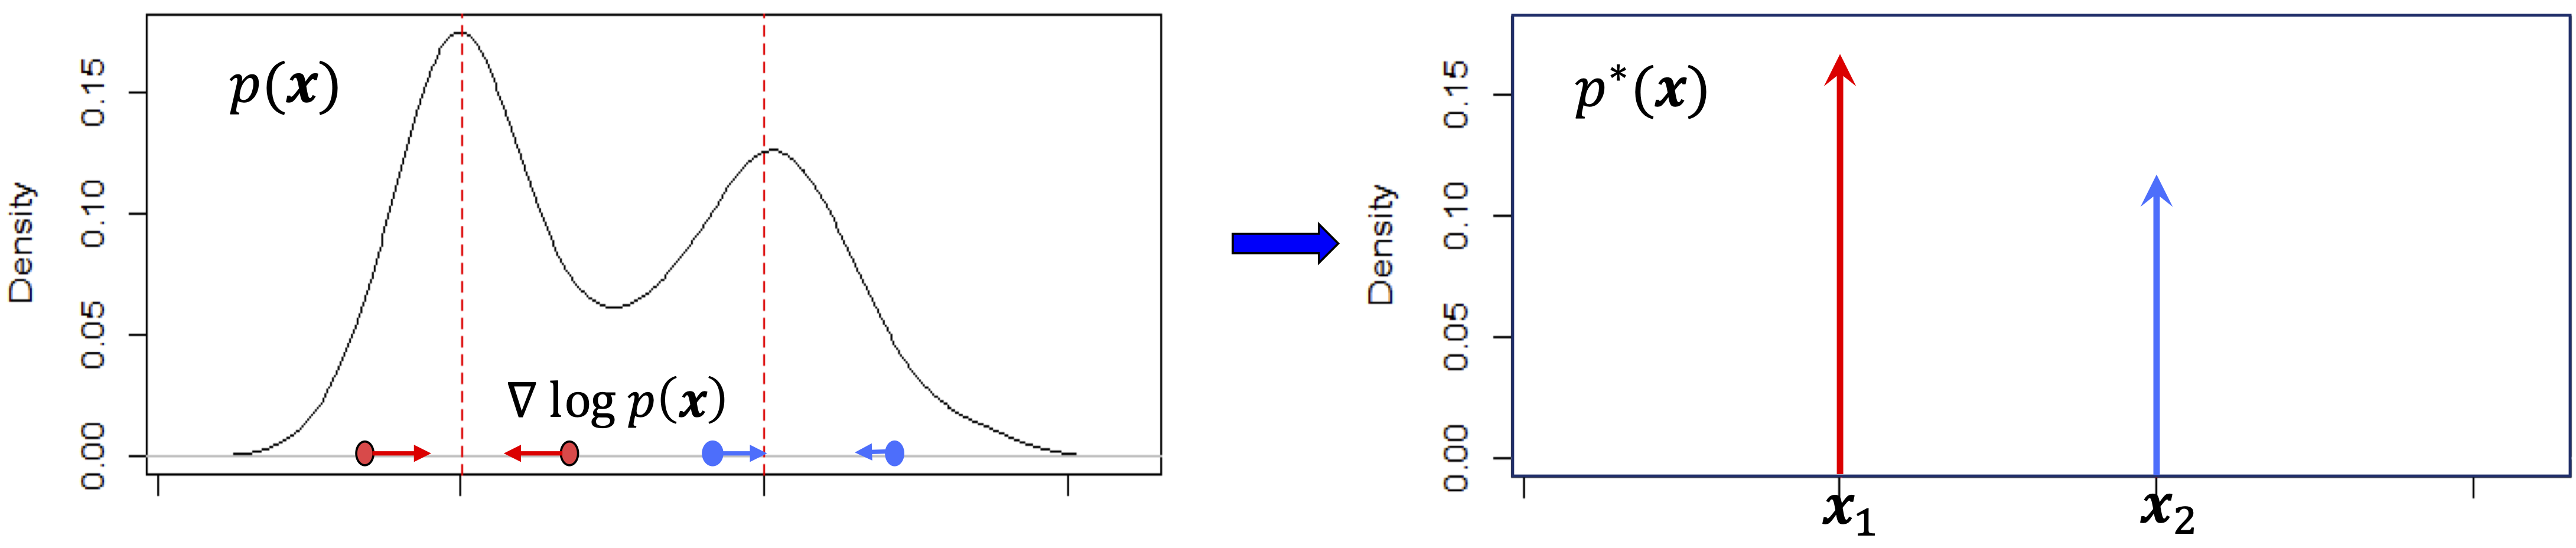
\includegraphics[width=1\linewidth]{\toplevelprefix/chapters/chapter1/figs/Density-compress.png}
    \caption{Geometric interpretation of a score function $\nabla \log p(\x)$ for a distribution with density $p(\x)$ on the left. The operation generated by the score function pushes the distribution towards areas of higher density. The goal is that, by a certain measure of compactness (e.g. entropy or coding length), the resulting distribution is more ``compressed''. Eventually, the distribution converges onto one that is with a lower-dimensional support, as $p^*(\x)$ shown on the right.}
    \label{fig:score-function}
\end{figure}

\paragraph{Entropy minimization.} In fact, this function has a very intuitive information-theoretic and geometric interpretation. Note that in information theory $-\log p(\x)$ generally corresponds to the number of bits needed to encode $\x$\footnote{at least in the case of a discrete variable, as we will explain in more details in Chapter \ref{ch:compression}.}. The gradient $\nabla \log p(\x)$  points to a direction in which the density is higher, as shown in Figure \ref{fig:score-function} left. The number of bits needed to encode $\x$ decreases if it moves in that direction. Hence, the overall effect of the operator $\nabla \log p(\x)$ is to push the distribution to ``shrink''  towards areas of higher density. Actually, one can formally show that the (differential) entropy of the distribution 
\begin{equation}
H(\x) = - \int p(\boldsymbol{w}) \log p(\boldsymbol{w}) \odif{\boldsymbol{w}}    \end{equation} 
indeed decreases under such an operation (see Chapter \ref{ch:compression} and Appendix \ref{app:diffusion-denoising}). Therefore, if we encode it with an optimal code book, the overall coding length/rate of the resulting distribution is reduced, hence more ``compressed.''. Intuitively, one can imagine that, if we repeat such a denoising process indefinitely, the distribution will eventually shrunk to one whose mass is concentrated on a support of lower dimension. For example, the distribution $p(\x)$ shown on the left of Figure \ref{fig:score-function},  under the action of the score function $\nabla \log p(\x)$, eventually will converge to the distribution $p^*(\x)$ on the right\footnote{Strictly speaking, $p^*(\x)$ is a distribution whose density is a generalized function: $p^*(\x) = p^*(\x_1)\delta(\x-\x_1) + p^*(\x_2) \delta(\x-\x_2)$, with $p^*(\x_1) + p^*(\x_2) = 1$. }:
\begin{equation}
H(\x) = - \int p(\boldsymbol{w}) \log p(\boldsymbol{w}) \odif{\boldsymbol{w}}  \quad \xrightarrow{\hspace{1mm} \mbox{decreasing} \hspace{1mm}} \quad H^*(\x) = - \int p^*(\boldsymbol{w}) \log p^*(\boldsymbol{w}) \odif{\boldsymbol{w}}.    
\end{equation}
Strictly speaking, as the distribution converges to $p^*(\x)$, it differential entropy converges to negative infinity. This is due to a technical difference between the definition of differential entropy for continuous random variable and discrete random variable, respectively. We will see how to resolve this technical difficulty in Chapter \ref{ch:compression}, using a more uniform measure of {\em rate distortion}.


We will discuss later in this chapter and in Chapter \ref{ch:compression}, how such a seemingly simple concept of denoising and compression leads to a very unifying and powerful method for learning general low-dimensional distributions in a high-dimensional space, including the distribution of natural images. 

\subsection{Empirical Approaches}
In practice, for many important real-world data such as images, sounds, and texts, it is difficult to model them with idealistic linear or mixed linear models. For example, there has been a long and rich history in the fields of image processing and computer vision that tries to model the distribution of natural images analytically. David Mumford, a Fields Medalist, spent considerable effort in the 1990s trying to understand and model the statistics of natural images \cite{Mumford1996TheSD}. He and his students, including Song-Chun Zhu, drew inspiration and techniques from statistical physics and proposed many statistical and stochastic models for the distribution of natural images \cite{Zhu-Entropy-1997,Zhu1997LearningGP,Zhu1997Prior,Huang-Mumford,Mumford-1999,Lee-Mumford}. However, these analytical models met with limited success in producing samples that closely resemble natural images. Obviously, for real-world data like images, we need to develop more powerful and unifying methods to pursue their more general low-dimensional structures.

Hence, historically, many empirical models  have been proposed to model important real-world data, including images and texts. These models often drew inspiration from the characteristics of the biological nerve system because the brain of an animal or human seems to process these data extremely efficiently and effectively. 

\subsubsection{Classic Artificial Neural Networks}
\paragraph{Artificial neuron.}

\begin{figure}[t]
    \centering
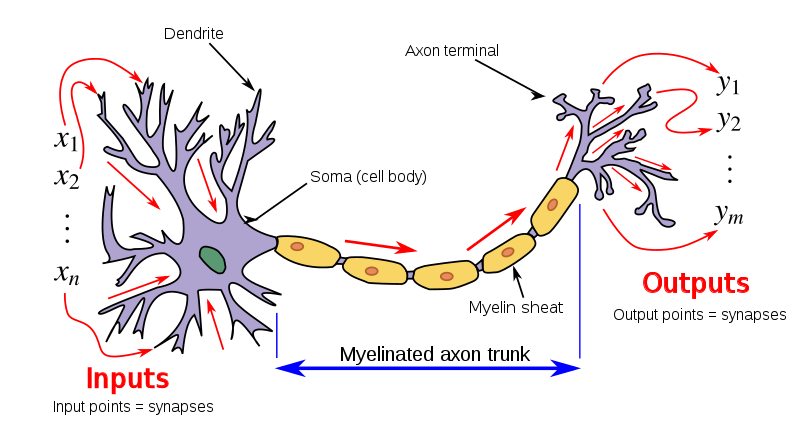
\includegraphics[width=0.55\linewidth]{\toplevelprefix/chapters/chapter1/figs/neuron.png} \hspace{3mm}   
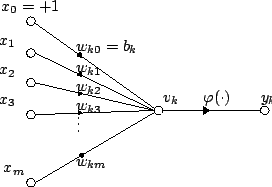
\includegraphics[width=0.40\linewidth]{\toplevelprefix/chapters/chapter1/figs/Artificial_neuron.png}
    \caption{The first mathematical model of an artificial neuron (right) that emulates how a neuron (left) processes signals. }
    \label{fig:neuron}
\end{figure}

Inspired by the nerve system in the brain, the mathematical model of the first artificial neuron\footnote{known as the  Linear Threshold Unit, or a perceptron.} was proposed by Warren McCulloch\footnote{A professor of psychiatry at the University of Chicago at the time} and Walter Pitts in 1943 \cite{McCulloch-Pitts}. It describes the relationship between the input $x_i$ and output $o_j$ as:
\begin{equation}
    o_j = \varphi\Big( \sum_i w_{ji}x_i\Big),  
\end{equation}
where $\varphi(\cdot)$ is some nonlinear activation, normally modeled by a threshold function. This model is illustrated in Figure \ref{fig:neuron}. As we can see, this form already shares the main characteristics of a basic unit in modern deep neural networks. The model is derived from observations of how a single neuron works in our nerve system. However, people did not know exactly what functions a collection of such neurons wants to realize and perform. On a more technical level, neither were they sure what nonlinear activation function $\varphi(\cdot)$ should be used. Hence, historically many variants have been proposed.\footnote{Step function, Hard or soft thresholding, Rectified Linear Unit (ReLU), sigmoid, etc.
}

\begin{figure}[t]
\centering
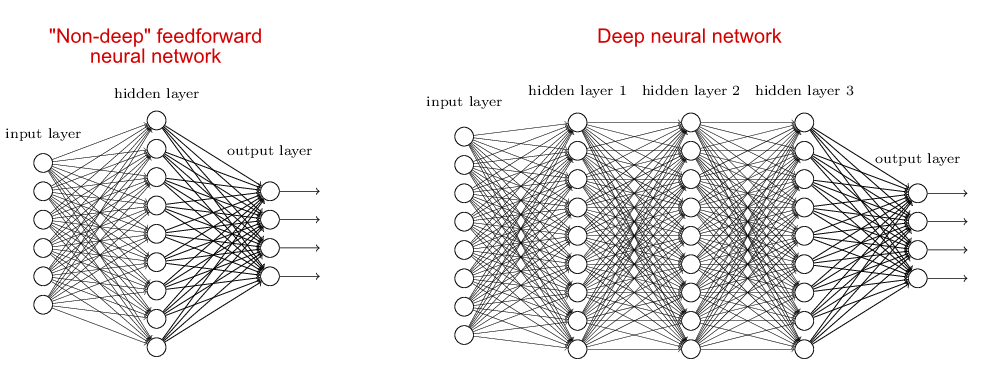
\includegraphics[width=0.85\linewidth]{\toplevelprefix/chapters/chapter1/figs/single-deep.png}
    \caption{A network with one single hidden layer (left) versus a deep network (right).  }
    \label{fig:single-deep}
\end{figure}
\paragraph{Artificial neural network.}
In the 1950s, Frank Rosenblatt was the first to build a machine with a {\em network} of such artificial neurons, shown in Figure \ref{fig:perceptron}. The machine is called Mark I Perceptron which consists of an input layer, an output layer, and a single hidden layer consisting of 512 artificial neurons, as shown in Figure \ref{fig:perceptron} left,  which is similar to what is illustrated in Figure \ref{fig:single-deep} left. It was designed to classify optical images of letters. However, the capacity of a single-layer network is limited and can only learn linearly separable patterns. In a 1969 book {\em Perceptrons: An Introduction to Computational Geometry} by Marvin Minsky and Seymour Papert \cite{Minsky-1969}, it was shown that the single-layer architecture of Mark I Perceptron cannot learn an XOR function. This result had significantly damped people's interest in artificial neural networks, even though it was later proven that a multi-layer network is able to learn an XOR function \cite{Rumelhart1986}. In fact, a (big enough) multi-layer network, as shown in Figure \ref{fig:single-deep} right,  consisting of such simple neurons can simulate any finite-state machine, even the universal Turing machine.\footnote{Do not confuse what neural networks are  capable of doing in principle with whether it is tractable or easy to learn a neural network that realizes certain desired functions.}  Nevertheless, subsequently, the study of artificial neural networks went into its first winter in the 1970s.

\begin{figure}
    \centering
    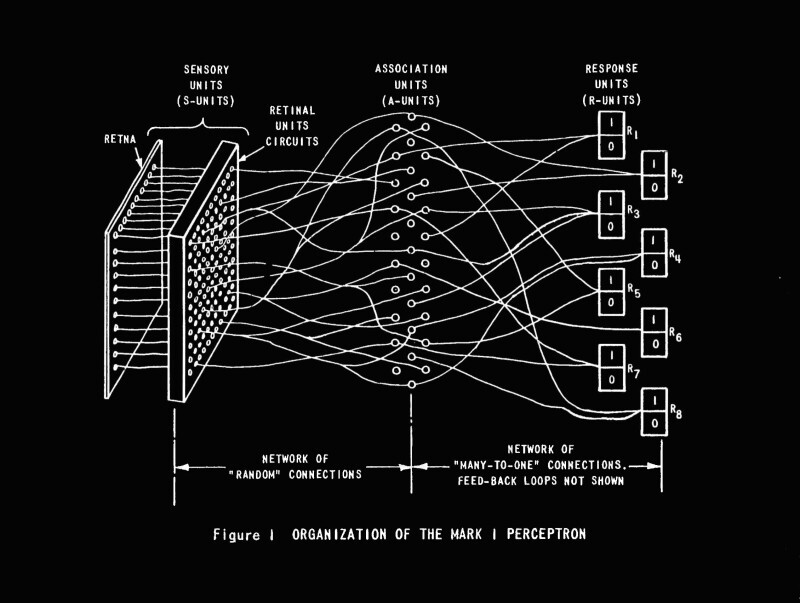
\includegraphics[width=0.45\linewidth]{\toplevelprefix/chapters/chapter1/figs/visu-large.jpg}
    \hspace{2mm} 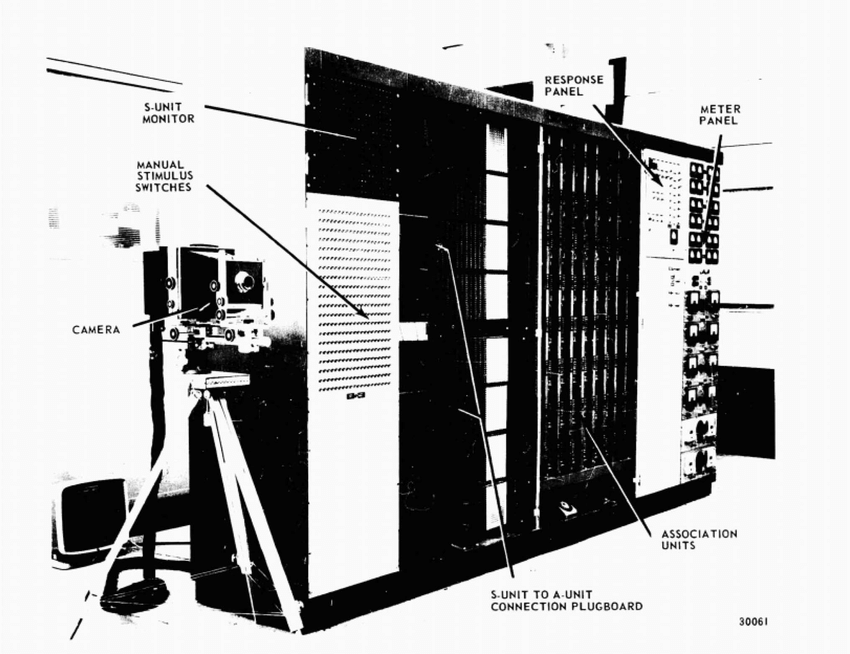
\includegraphics[width=0.45\linewidth]{\toplevelprefix/chapters/chapter1/figs/Original-Mark-I-perceptron-as-seen-in-its-operators-manual-20.ppm.png}
    \caption{The Mark I Perceptron machine developed by Frank Rosenblatt in late 1950s.}
    \label{fig:perceptron}
\end{figure}


\paragraph{Convolutional neural networks.}
The somewhat disappointing early experimentation with artificial neural networks like Mark I Perceptron in the 50s and 60s suggested that it might not be enough to simply connect neurons in a general fashion as multi-layer perceptrons (MLP). In order to build effective and efficient networks, we need to understand what purpose or function neurons in a network need to achieve collectively so that they should be organized and learned in a certain special way. Once again, the study of machine intelligence turned to draw inspiration from how the animal's nerve system works. 

It is known that most of our brain is dedicated to process visual information. In 1950s and 1960s, David Hubel and Torsten Wiesel systematically studied the visual cortices of cats. It was discovered that the visual cortex contains different types of cells (known as simple cells and complex cells), which are sensitive to visual stimuli of different orientations and locations \cite{Hubel-Wiesel-1959}. Hubel and Wiesel won the 1981 Nobel Prize in Physiology or Medicine for their ground-breaking discovery. 


On the artificial neural network side, Hubel and Wiesel's work had inspired Kunihiko Fukushima who  designed the ``neocognitron'' network in 1980 which consists of artificial neurons that emulate biological neurons in the visual cortices \cite{Fukushima1980NeocognitronAS}. This is known as the first {\em convolutional neural network} (CNN), and its architecture is illustrated in Figure \ref{fig:neocognitron}. Unlike the perceptron, the neocognitron had more than one hidden layer and could be viewed as a deep network, as compared in Figure \ref{fig:single-deep} right.

Also inspired by how neurons work in the cat's visual cortex, he was also the first to introduce the use of {\em rectified linear unit} (ReLU):
\begin{equation}
    \varphi(x) = \max\{0, x\} = \casework{x, & \text{if} \, x > 0, \\ 0, \quad & \text{if} \, x \leq 0,}
\end{equation}
for the activation function $\varphi(\cdot)$ in 1969 \cite{Fukushima-1969}. But not until recent years has the ReLU become widely used activation function in modern deep (convolutional) neural networks. We will learn from this book why this is a good choice once we explain the main operations that deep networks try to implement: compression. 
%\yima{An image of a convolution neural network or the LeNet here...}

\begin{figure}
    \centering
    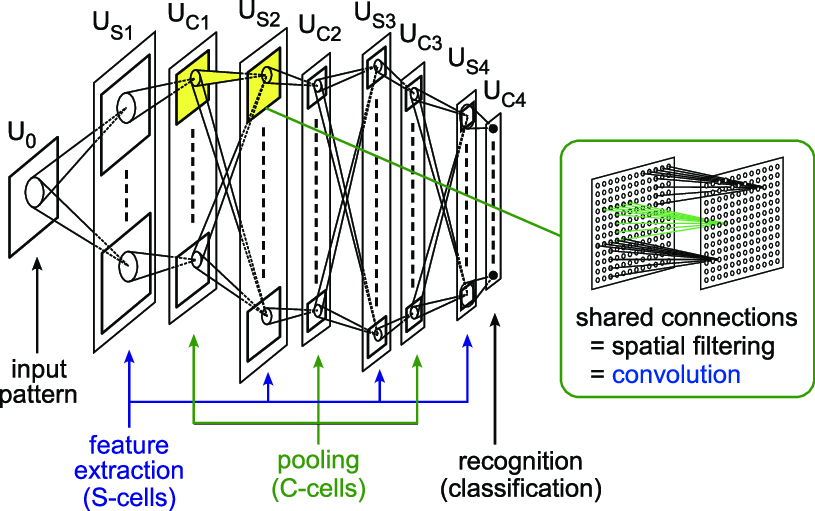
\includegraphics[width=0.6\linewidth]{\toplevelprefix/chapters/chapter1/figs/neocognitron.png}
    \caption{Origin of convolutional neural networks: the Neocognitron by Kunihiko Fukushim in 1980. Notice that the interleaving layers of convolutions and pooling try to emulate the functions of simple cells and complex cells discovered in the visual cortices of cats.}
    \label{fig:neocognitron}
\end{figure}

CNN-type networks continued to evolve in the 1980s and many different variants had been introduced and studied. However, despite the remarkable capacities of deep networks and the improved architectures inspired by neuroscience, it remained extremely difficult to train such deep networks for a real task such as image classification. How to get a network to work depended on many unexplainable heuristics and tricks that really limited the appeal and applicability of neural networks. One major breakthrough came around 1989 when Yann LeCun successfully used {\em back propagation} (BP) to learn a deep convolutional neural network for recognizing hand-written digits \cite{LeCun-1989}, later known as the LeNet (see Figure \ref{fig:LeNet-5}). After several years' persistent development, his perseverance paid off: performance of the LeNet eventually became good enough for practical usage in late 1990s \cite{LeCun-1998}: it was used by the US Post Office for recognizing handwritten digits (for zip codes).  The LeNet was considered as the ``prototype'' network for all modern deep neural networks, such as the AlexNet and ResNet, which we will discuss later. Due to this work, Yann LeCun was awarded the 2018 Turing Award.\footnote{Together with two other pioneers of deep networks, Yoshua Bengio and Geoffrey Hinton.}

\begin{figure}
    \centering
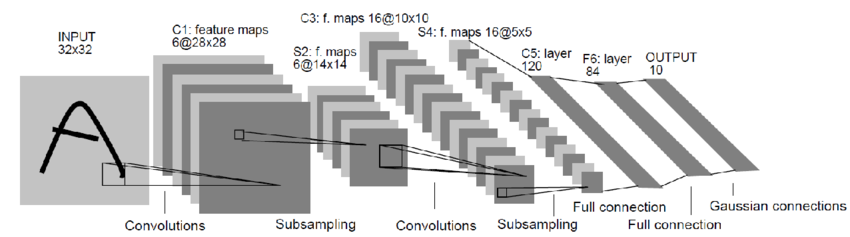
\includegraphics[width=0.95\linewidth]{\toplevelprefix/chapters/chapter1/figs/LeNet-5.png}
    \caption{The LeNet-5 convolution neural network designed by Yann LeCun in 1989. }
    \label{fig:LeNet-5}
\end{figure}

\paragraph{Backpropagation.}
In history, the fate of deep neural networks seems to be tied closely to how they can be trained easily and efficiently. Back propagation (BP) was introduced for this reason. We know that a multiple layer perceptron can be expressed as a  composition of a sequence of linear mappings and nonlinear activations as follows:
\begin{equation}
h(\bm W_1, \ldots, \bm W_L) = f^L(\bm W_Lf^{L-1}(\bm W_{L-1} \cdots f^2(\bm W_2f^1(\bm W_1\x)))).
\end{equation}
In order to train the network weights $\{\bm W_l\}_{l=1}^L$ to reduce the prediction/classification error based on a gradient descent algorithm, we need to evaluate the gradient ${\partial h}/{\partial \bm W_l}$. It has been well known, from the {\em chain rule} in calculus, that gradients can be computed efficiently for this type of functions, later known as back propagation (BP). See Appendix \ref{app:optimization} for a detailed description. The technique of back propagation was already known and practiced by people in fields such as optimal control and dynamic programming in the 1960s and 1970s. For example, it appeared in the 1974 PhD thesis of Dr. Paul Werbos \cite{Werbos-1974, Werbos1994TheRO}. In 1986, David Rumelhart et al. were the first to apply back propagation  to train a multiple layer perceptron (MLP) network \cite{Rumelhart1986}. Since then,  BP has become increasingly popular since it gives a {\em scalable} algorithm to learn large deep neural networks.\footnote{as it can be efficiently implemented on computing platforms that facilitate parallel and distributed computing.} It is now an almost dominant technique for training deep neural networks today. However, it is believed that nature does not learn by back propagation,  because such a mechanism is still way too expensive for physical implementation by nature\footnote{As we have discussed earlier, nature almost ubiquitously learns to correct error via closed-loop feedback.}. This obviously leaves tremendous room for improvement in the future, as we will discuss more.

However, despite the above algorithmic progress and promising practice in the 1980s, training deep neural networks remained extremely finicky and expensive for computing systems in the 1980s and 1990s. In late 1990s, support vector machines (SVM) \cite{SVM-1995} had become very popular as they were viewed as a better alternative to neural networks for tasks such as classification.\footnote{In fact, similar ideas to solve classification problems can be traced back to the PhD dissertation work of Thomas Cover, which as condensed and published in a paper in 1964  \cite{Cover-1964}.} There were two main reasons: first, SVM was based on a rigorous statistical learning framework known as the Vapnik--Chervonenkis (VC) theory; and second, it leads to rather efficient algorithms based on convex optimization \cite{BoydVa04}. The rise of SVM had brought a second winter to the study of neural networks around the early 2000s. 

\paragraph{Compressive autoencoding.}
In the late 1980s and 1990s, artificial neural networks were already adopted to learn low-dimensional representations of high-dimensional data such as images. It had been shown that neural networks can be used to learn PCA from the data \cite{Oja1982SimplifiedNM,Baldi89}, instead of using the classic methods discussed in Section \ref{sec:PCA-ICA}. It was also argued during late 1980s that due to its capability to model nonlinear transforms, neural networks were suggested to learn low-dimensional representations for data with nonlinear distributions. Similar to the linear PCA case, one can try to simultaneously learn a nonlinear dimension-reduction encoder $f$ and a decoder $g$, each modeled by a deep neural network  \cite{Rumelhart1986,Kramer1991NonlinearPC}:
\begin{equation}
    \X   \xrightarrow{\hspace{2mm} f \hspace{2mm}} \Z  \xrightarrow{\hspace{2mm} g \hspace{2mm}} \hat \X.
       \label{eqn:auto-encoding-deep-networks}
\end{equation}
By enforcing the decoded data $\hat \X$ to be consistent with the original $\X$, say by minimizing an MMSE type reconstruction error\footnote{Although MMSE type of errors are known to be problematic to imagery data that have complex nonlinear structures. As we will soon discuss, much of the recent work in generative methods, including GANs, has been to find surrogates of better distance functions between the original data $\X$ and the regenerated $\hat \X$.}:
\begin{equation}
    \min_{f,g} \big\|\X - \hat \X\big\|_2^2 = \big\|\X - g(f( \X))\big\|_2^2,
\end{equation}
an autoencoder can be learned from the data $\X$ themselves. 

But how can we guarantee that such an autoencoding indeed captures the true low-dimensional structures in $\X$ instead of giving a trivial redundant representation? For example, we can simply choose $f$ and $g$ to be the identity map and $\Z = \X$. So to ensure the autoencoding to be worthwhile, one wishes the resulting representation to be compressive, in terms of a certain computable measure of complexity. In 1993, Geoffrey Hinton and colleagues proposed to use the coding length as such a measure, hence the objective of autoencoding became to find such a representation that minimizes the coding length \cite{Hinton-1993}. This work also established a fundamental connection between the principle of minimum description length \cite{Rissanen-1978} and free (Helmholtz) energy minimization. Later work \cite{Hinton504} from Hinton's group showed empirically that such an autoencoding is capable of learning meaningful low-dimensional representations for real-world images. A more comprehensive survey of autoencoders was done by Pierre Baldi in 2011 \cite{Baldi2011}, just before deep networks became popular. We will discuss more about the measure of complexity and autoencoding later in Section \ref{sec:unifying-approach}, and give a systematic study of compressive autoencoding to Chapter \ref{ch:consistent}, with a more unifying view.


\begin{figure}
    \centering
    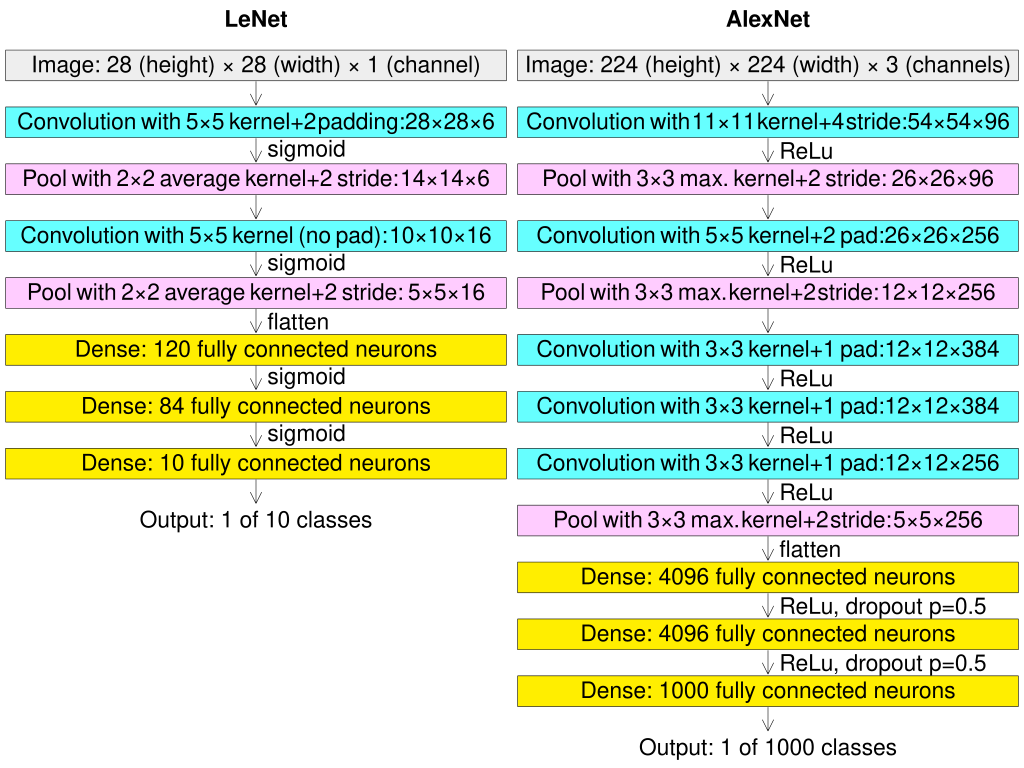
\includegraphics[width=0.8\linewidth]{\toplevelprefix/chapters/chapter1/figs/Comparison_image_neural_networks.svg.png}
    \caption{Architecture of the LeNet \cite{LeCun-1989} versus that of the AlexNet \cite{krizhevsky2012imagenet}.}
    \label{fig:LeNet-AlexNet}
\end{figure}


\subsubsection{Modern Deep Neural Networks}
For nearly 30 years, from 1980s to 2010s, for the study of machine learning and machine intelligence, neural networks were not considered seriously by the mainstream. Early (deep) neural networks, such as the LeNet, have shown promising performance for small-scale classification problems such as recognizing digits. However, the design and practice of the networks were rather empirical, datasets available at the time were small, and the BP algorithm was a huge computational burden for computers then. These factors had resulted in the lack of interest in neural networks, and progress had been stagnant, with only a handful of researchers working on it. 

\paragraph{Classification and recognition.}
As it turns out, the tremendous potential of deep neural networks could only be unleashed once there are enough data and computing power. Fast forward to 2010s, much larger datasets such as ImageNet became available, and GPUs became powerful enough to make BP much more affordable, even for networks much larger than LeNet. Around 2012, a deep convolutional neural network known as the AlexNet drew attention as it surpassed extent classification methods by a significant margin with the ImageNet dataset \cite{krizhevsky2012imagenet}.\footnote{In fact, before this, deep networks had demonstrated state of the art performance on speech recognition tasks. But it did not receive so much attention till their success with image classification.} Figure \ref{fig:LeNet-AlexNet} shows the comparison between the AlexNet and the LeNet. The AlexNet shares many common characteristics as the LeNet, only it is bigger and has adopted ReLU as the nonlinear activation instead of the Sigmoid function used in LeNet. Partly due to the influence of this work, Geoffrey Hinton was awarded the 2018 Turing Award.


This early success inspired the machine intelligence community, in the next few years, to explore new variations and improvements to the network design. In particular, people had discovered empirically that the larger and deeper the networks, the better the performance in tasks such as image classification. Many deep network architectures have been tried, tested, and popularized. A few notable ones include VGG \cite{Simonyan15}, GoogLeNet \cite{Szegedy2014GoingDW}, ResNet \cite{He2016-lc}, and more recently Transformers \cite{vaswani2017attention} etc. Despite fast progress in empirical performance, there was a lack of theoretical explanation for these empirically discovered architectures, including relationships among them if any. One purpose of this book is to reveal what common objective all these networks may serve and why they share certain common characteristics, including multiple layers of linear operator interleaved with nonlinear activation (see Chapter \ref{ch:representation}). 

\paragraph{Reinforcement learning.}
The early successes of deep networks were mainly for classification tasks in a supervised learning setting, such as speech recognition and image recognition. Deep networks were later adopted by the DeepMind team, led by Demis Hassabis, to learn decision-making or control policies for playing games. In this context, deep networks are used to model the optimal decision/control policy or the associated optimal value function, as shown in Figure \ref{fig:Alpha-Go}. These network parameters are incrementally optimized \footnote{Say based on back propagation (BP).} based on reward returned from the success or failure of playing the game with the current policy. This learning method is generally referred to as {\em reinforcement learning} \cite{Sutton-Barto}, originated from the practice of control systems in the late 1960s \cite{Waltz1965AHA,Mendel1970ReinforcementlearningCA}. Its earlier roots can be traced back to a much longer and richer history of {\em dynamic programming} by Richard Bellman \cite{Bellman-DP} and {\em trial-and-error learning} by Marvin Minsky \cite{Minsky-1954} in the 1950s. 

From an implementation perspective, the combination of deep networks and reinforcement learning turned out to be rather powerful: deep networks can be used to approximate control policy and value function for real-world environments that are difficult to model analytically. This practice had eventually led to the AlphaGo system, developed by the company DeepMind, which surprised the world in 2016 by beating a top human player Lee Sedol in the game Go and then the world champion Jie Ke in 2017.\footnote{In 1996, IBM's Deep Blue system made history by defeating Russian grandmaster Garry Kasparov in chess. It mainly used traditional machine learning techniques, such as tree search and pruning, which were not so scalable and had not been proven successful for more challenging games such as Go for over 20 years.} 

The success of AlphaGo came as a big surprise to the computing society which generally believes that the state space for search is too prohibitively large to admit any efficient solution, in terms of computation and sample size. The only reasonable explanation for its success is that there must be very good structures in the optimal value/policy function of the game Go. Their intrinsic dimension is not so high and they can be approximated well by a neural network, learnable from not so prohibitively many samples. 

\begin{figure}
    \centering
    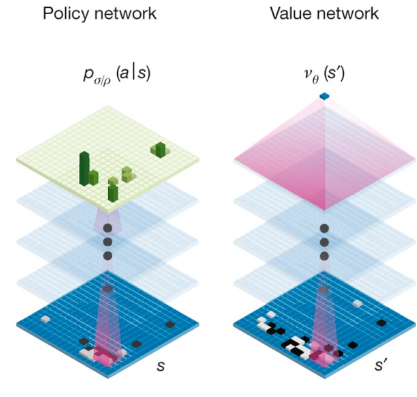
\includegraphics[width=0.5\linewidth]{\toplevelprefix/chapters/chapter1/figs/Policy-Value.png}
    \caption{AlphaGo: Using deep neural networks to model the optimal policy or the optimal value function for the game Go. }
    \label{fig:Alpha-Go}
\end{figure}

\paragraph{Generation and prediction.}
One may view early practices of deep networks in the 2010s focused more on extracting relevant information from the data $\X$ and encoding it for certain task-specific representation $\Z$ (say $\Z$ represent class labels in classification tasks):
\begin{equation}
    \X   \xrightarrow{\hspace{2mm} f \hspace{2mm}} \Z.
       \label{eqn:encoding-deep-networks}
\end{equation}
In this setting, the mapping $f$ to be learned does not need to preserve most  distributional information about $\X$ but only the sufficient statistics needed for a specific task. For example, a sample $\x$ in $\X$ could be an image of an apple, which is mapped by $f$ to its class label $\z =$ ``apple.'' The {\em information bottleneck framework} \cite{Tishby-ITW2015} was proposed in 2015 to analyze the role of deep networks in such a context.
 
However, in many modern situations such as those so-called large foundation models,  people often need to decode $\Z$ to recover the corresponding $\X$ to a certain degree of precision:
\begin{equation}
    \Z   \xrightarrow{\hspace{2mm} g  \hspace{2mm}} \hat \X.
       \label{eqn:decoding-deep-networks}
\end{equation}
As $\X$ typically represents data observed from the external world, a good decoder would allow us to simulate or predict what happens in the world. For example, in a ``text to image'' or ``text to video'' task, $\z$ normally represents the texts that describe the content of a desired image $\x$. The decoder should be able to generate an $\hat \x$ that has the same content as $\x$. For example, given an object class $\z = $ ``apple'', the decoder $g$ should generate an image $\hat \x$ that looks like an apple, although not necessarily exactly the same as the original $\x$. 



\paragraph{Generation via discriminative approaches.}
In order for the generated images $\hat \X$ to be similar to the true natural images $\X$, we need to be able to evaluate and minimize some distance:
\begin{equation}
    \min d(\X, \hat \X).
\end{equation}
As it turns out, most theoretically motivated  distances are extremely difficult, if not impossible, to compute and optimize for distributions in high-dimensional space but with a low intrinsic dimension.\footnote{This is the case even if a parametric family of distribution for $\X$ is given. The distance often becomes ill-conditioned or ill-defined for distributions with low-dimensional supports. What could be even worse is that the chosen family might not be able to approximate well the true distribution of interest.} 

In 2007, Zhuowen Tu, a former student of Song-Chun Zhu, probably disappointed by early analytical attempts to model and generate natural images (discussed earlier), decided to try a drastically different approach. In a paper published in CVPR 2007 \cite{Tu-2007}, he was the first to suggest that one could learn a generative model for images via a discriminative approach. The idea is simple: if it is difficult to evaluate the distance $d(\X, \hat \X)$, one could try to  learn a discriminator $d$ to separate $\hat \X$ from $\X$: 
\begin{equation}
    \Z   \xrightarrow{\hspace{2mm} g  \hspace{2mm}} \hat \X, \X \xrightarrow{\hspace{2mm} d  \hspace{2mm}} \boldsymbol{0}, \boldsymbol{1},
       \label{eqn:gan-networks}
\end{equation}
where $\boldsymbol{0}, \boldsymbol{1}$ indicate an image is generated or not.
Intuitively, the harder we could separate $\hat \X$ and   $\X$, probably the closer they are. 

Tu's work \cite{Tu-2007} was the first to demonstrate the feasibility of learning a generative model from a discriminative approach. However, the work adopted traditional methods to generate images and classify distributions (such as boosting), and they were slow and hard to implement. After 2012, deep neural networks became very popular for image classification. In 2014, Ian Goodfellow and colleagues proposed again to generate natural images with a discriminative approach \cite{Goodfellow-2014}. They suggested using deep neural networks to model the generator $g$ and the discriminator $d$ instead. Moreover, they proposed to learn the generator $g$ and discriminator $d$ via a minimax game:
\begin{equation}
    \min_g \max_d \ell(\X, \hat \X),
\end{equation}
where $\ell(\cdot)$ is some natural loss function associated with the classification.  In words the discriminator $d$ tries to maximize its success in separating $\X$ and $\hat \X$, whereas the generator $g$ tries to do the opposite. For this reason, this approach is named as {\em generative adversarial networks} (GANs). It was shown that once trained on a large dataset, GANs can indeed generate photo-realistic images. Partially due to the influence of this work, Yoshua Bengio was awarded the 2018 Turing Award.

The discriminative approach seems to be a rather clever way to bypass a fundamental difficulty in distribution learning. However, rigorously speaking, this approach does not fully resolve this fundamental difficulty at all. It is shown by  \cite{Goodfellow-2014} that with a properly chosen loss, the minimax formulation is mathematically equivalent to minimize {\em the Jensen-Shannon distance} (see \cite{Cover-Thomas}) between $\X$ and $\hat \X$. This is known to be a hard problem for two low-dimensional distributions in a high-dimensional space. As a result, in practice, GANs typically rely on many heuristics and engineering tricks and often suffer from instability issues such as {\em mode collapsing}.\footnote{Nevertheless, such a minimax formulation provides a practical approximation of the distance. It simplifies the implementation and avoids certain caveats in directly computing the distance.} Overall, there has been a lack of theoretical guidance on how to improve the practice of GANs.

\paragraph{Generation via denoising and diffusion.}
In 2015, shortly after GAN was introduced and became popular, Surya Ganguli and his students realized and suggested that an iterative denoising process modeled by a deep network can be used to learn a general distribution, such as that of natural images \cite{Sohl-Dickstein2015}. Their method was inspired by properties of the special Gaussian and binomial processes, studied by William Feller back in 1949 \cite{Feller1949OnTT}.\footnote{Again, in the magical era of 1940s!} 

\begin{figure}[t]
    \centering
    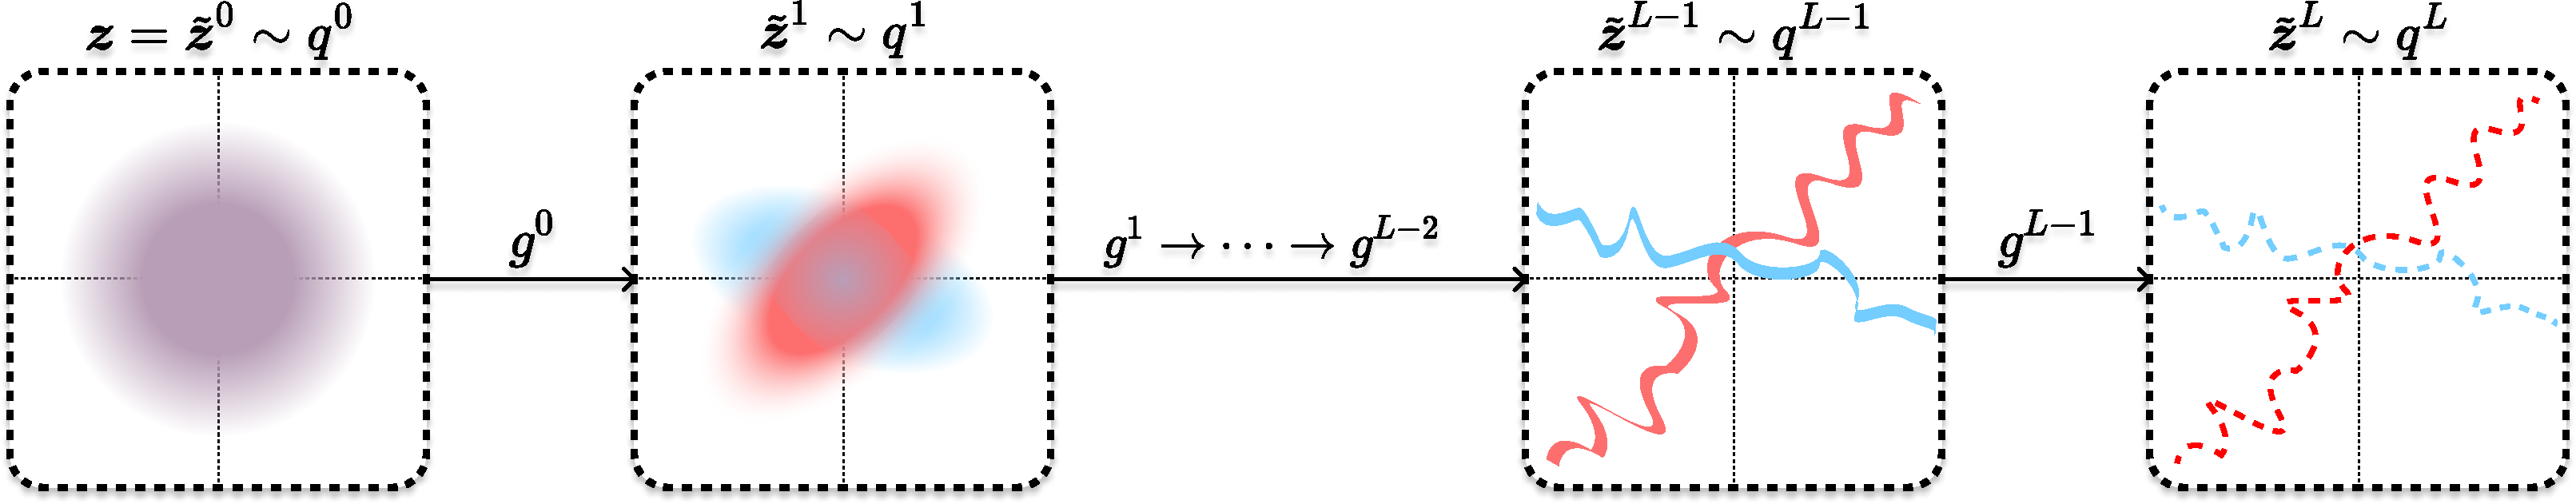
\includegraphics[width=\linewidth]{\toplevelprefix/chapters/chapter1/figs/diffusion_pipeline-2.pdf}
    \caption{Illustration of an iterative denoising and compressing process that, starting from a Gaussian distribution $q^0 = \mathcal{N}(\boldsymbol{0}, \boldsymbol{I})$, converges to an arbitrary low-dimensional data distribution $q^L = p(\x)$. }
    \label{fig:diffusion}
\end{figure}

Soon, denoising operators based on the score function \cite{hyvarinen05a}, briefly introduced in Section \ref{sec:denoising-intro}, were shown to be more general and unified the denoising and diffusion processes and algorithms \cite{song2019,song2020score,ho2020denoising}. Figure \ref{fig:diffusion} gives an illustration of the process that transforms a generic Gaussian distribution $q^0 = \mathcal{N}(\boldsymbol{0}, \boldsymbol{I})$ to an (arbitrary) empirical distribution $p(\x)$ by performing a sequence of iterative denoising (or compressing) operations:
\begin{equation}
        \z^0 \sim  \mathcal{N}(\boldsymbol{0}, \boldsymbol{I})\xrightarrow{\hspace{2mm} g^0  \hspace{2mm}} \z^1 \xrightarrow{\hspace{2mm} g^1 \hspace{2mm}} \cdots \xrightarrow{\hspace{2mm} g^{L-1}  \hspace{2mm}} \z^L \sim p(\x).
\end{equation}
By now, denoising (and diffusion) have replaced GANs and become a mainstream method for learning distributions of images and videos, leading to popular commercial image generating engines such as Midjourney and Stability.ai. 
In Chapter \ref{ch:compression} we will systematically introduce and study the denoising and diffusion method for learning a general low-dimensional distribution.  



\section{A Unifying Approach}\label{sec:unifying-approach}
So far, we have given a brief account of the main objective and history of machine intelligence and many important ideas and approaches associated with it. In recent years, after the empirical success of deep neural networks, tremendous efforts have been made to develop theoretical frameworks that can help us understand all the empirically designed deep neural networks, either certain seemingly necessary components (e.g., dropout,  normalization, attention, etc.) or their overall behaviors (e.g., double descent, neural collapse,  etc.). 

Partly motivated by this, this book aims to achieve several important and challenging goals: 
\begin{itemize}
    \item Develop a theoretical framework that would allow us to derive rigorous mathematical interpretation of deep neural networks.
    \item Ensure correctness of the learned data distribution and consistency with the learned representation.
    \item Demonstrate that the framework can lead to performant architectures and can guide further improvements in practice.
\end{itemize}
Within the past few years, there is mounting evidence that these goals can indeed be achieved, by leveraging the theory and solutions to the classical analytical low-dimensional models discussed briefly earlier (more thoroughly in Chapter \ref{ch:classic}) and by integrating fundamental ideas from a few related fields, namely information/coding theory, control/game theory, and optimization. This book aims to give a systematic introduction to this new approach.

\subsection{Learning Parsimonious Representations}
\label{sec:computational-approach-compression}
One necessary condition for any  learning task to be possible is that the sequences of interest must be {\em computable}, at least in the sense of Alan Turing \cite{Turing-1936}. That is, a sequence can be computed via a program on a typical computer.\footnote{There are indeed well-defined sequences that are not computable.} In addition to being computable, we require computation be {\em tractable}.\footnote{We do not need to consider predicting things whose computational complexity is intractable, say grows exponentially in the length or dimension of the sequence.} That is, the computational cost (space and time) for learning and computing the sequence should not grow exponentially in length. Furthermore, as we see in nature (and in modern practice of machine intelligence), for most practical tasks, an intelligent system needs to learn what is predictable from massive data in a very high-dimensional space, such as from vision, sound, and touch. Hence, for intelligence, we do not need to consider all computable and tractable sequences or structures. We should focus only on predictable sequences and structures which admit {\em scalable} realizations of its learning and computing algorithms:
\begin{equation}
\mbox{\textbf{computable}} \;
   \Longrightarrow \; \mbox{\textbf{tractable}} \; \Longrightarrow \; 
   \mbox{\textbf{scalable}}.
\end{equation}

This is because whatever algorithms intelligent beings use to learn useful information must be {\em scalable}. More specifically, the computational complexity of the algorithms would better scale gracefully, typically linear or even sublinear, in the size and dimension of the data. On the technical level, this requires that the operations that the algorithms rely on to learn could only utilize oracle information that can be efficiently computed from the data. More specifically, when the dimension is high and the scale is large, the only oracle one could afford to compute is either the first-order geometric information about the data\footnote{such as approximating a nonlinear structure locally with linear subspaces and computing the gradient of an objective function.} or the second-order statistic information\footnote{such as covariance or correlation of the data or their features.}.
The main goal of this book is to develop a theoretical and computational framework within which we can systematically develop efficient and effective solutions or algorithms with such scalable oracles and operations to {\em learn} low-dimensional structures from the sampled data and subsequently the predictive function.


\paragraph{Pursuing low-dimensionality via compression.}
From the examples of sequences we gave in Section \ref{sec:predictability}, it is clear that some sequences are easy to model and compute and others are more difficult. Obviously, the computational cost of a sequence depends on how complex the predicting function $f$ is. The higher the degree of regression $d$, the more costly it is to compute. $f$ can be a simple linear function, and it can also be a nonlinear function that can be arbitrarily difficult to specify and compute. 

It is reasonable to believe that if a sequence is harder, by whatever measure we may choose, to specify and compute, then it will also be more difficult to learn from its sampled segments. Nevertheless, for any given predictable sequence, there are in fact many, often infinitely many, ways to specify it. For example, for a simple sequence $x_{n+1} = a x_{n}$, we could also define the same sequence with $x_{n+1} = a x_n + b x_{n-1} - b x_{n-1}.$
Hence it would be very useful if we could develop an objective and rigorous notion of ``complexity'' for any given computable sequence. 

Andrey Kolmogorov, a Russian mathematician, was one of the first to give a definition of complexity for any computable sequence.\footnote{Many have contributed to this notion of sequence complexity, most notably including Ray Solomonoff and Greg Chaitin. All three are believed to have developed and studied algorithmic information theory independently, Ray Solomonoff in 1960, Andrey Kolmogorov in 1965 \cite{Kolmogorov1998OnTO} and Gregory Chaitin around 1966 \cite{Chaitin-1966}.} He suggested that among all programs that can compute the same sequence, we may use the length of the shortest program as a measure for its complexity. This idea is very much in line with the famous ``Occam's Razor'' principle of parsimony: {\em one always chooses the simplest among all theories that can explain the same observation.} To be more precise, let $p$ represent a compute program that can generate a sequence $S$ on a universal computer $\mathcal{U}$. The  Kolmogorov complexity of the sequence $S$ is defined to be:
\begin{equation}
    K(S) = \min_{p\,:\, \mathcal{U}(p) = S} L(p). 
\end{equation}
Therefore, the complexity of a sequence is measured by how ``parsimonously'' we can specify or compute it. This definition of complexity, or parsimony, for sequences is of great conceptual importance and has many interesting properties. Historically, it has inspired many profound studies in the theory of computation, especially in the field of algorithmic information theory.

The length of the shortest program can be viewed as the ultimate compression of the sequence considered, providing a quantitative measure of how much we have gained by having learned the correct generative mechanism of the sequence. However, despite its theoretical importance, the Kolmogorov complexity is in general not a computable function \cite{Cover-Thomas} (even  intractable to approximate accurately). As a result, this measure of complexity is of little practical use. Neither can it tell us in advance how difficult it is to learn a given sequence nor can it tell us how well we have learned.





%Measure of parsimony or compactness: Many (largely equivalent) ways to measure compactness of data: Kolmogorov complexity (not computable), dimension and volume of (the support of) the data distribution, minimum description length, rate distortion etc. 

\paragraph{Computable measure of parsimony.}
Hence for practical purposes, we need an efficiently computable measure of complexity for sequences that are generated from the same predicting function.\footnote{Note that in practice, we typically care about learning the predicting function $f$, instead of any particular sequence generated by $f$.} Note that part of the reason why Kolmogorov complexity is not computable is because its definition is non-constructive.

So to introduce a computable measure of complexity, we may take a more constructive approach, as advocated by Claude Shannon through the framework of information theory \cite{Shannon-1948,Cover-Thomas}.\footnote{which has successfully guided the engineering practice of the communication industry for the past over 80 years.} In essence, by assuming the sequence $S$ is drawn from a probabilistic distribution $p(S)$, the so-called {\em entropy} of the distribution:\footnote{Here we consider differential entropy as we assume the sequence consists of continuous variables. If it consists of discrete variables, we could consider the entropy: $H(S) = - \sum_{i}p(s_i) \log p(s_i).$ }
\begin{equation}
    h(S) \doteq -\int p(s) \log p(s) \odif{s}
    \label{eqn:entropy-definition}
\end{equation}
gives a natural measure of its complexity. This measure also has a natural interpretation of the average number of binary bits needed to encode such a sequence, as we will see in Chapter \ref{ch:compression}.

To illustrate the main ideas of this view, let us take a large number of long sequence segments:
\begin{equation}
    \{S_1, S_2, \ldots, S_i, \ldots, S_N\} \subset \mathbb{R}^D,
\end{equation}
generated by a predicting function $f$. Note that without loss of generality, here we have assumed that all sequences are of the same length $D$. Therefore, each sequence can be viewed as a vector in $\mathbb{R}^D$. Secondly, we may introduce a coding scheme (with a code book), denoted as $\mathcal E$, that converts every segment $S_i$ to a unique stream of binary bits $\mathcal{E}(S_i)$. The simplest coding scheme is to fill the space spanned by all segments with $\epsilon$-balls, as shown in Figure \ref{fig:coding-schemes}. We then number all the balls. Each sequence is encoded as the (binary) number of its closest ball. Hence, each segment can be recovered\footnote{up to precision $\epsilon$ as such an encoding scheme is lossy.} from its corresponding bit stream. 
\begin{figure}
    \centering
    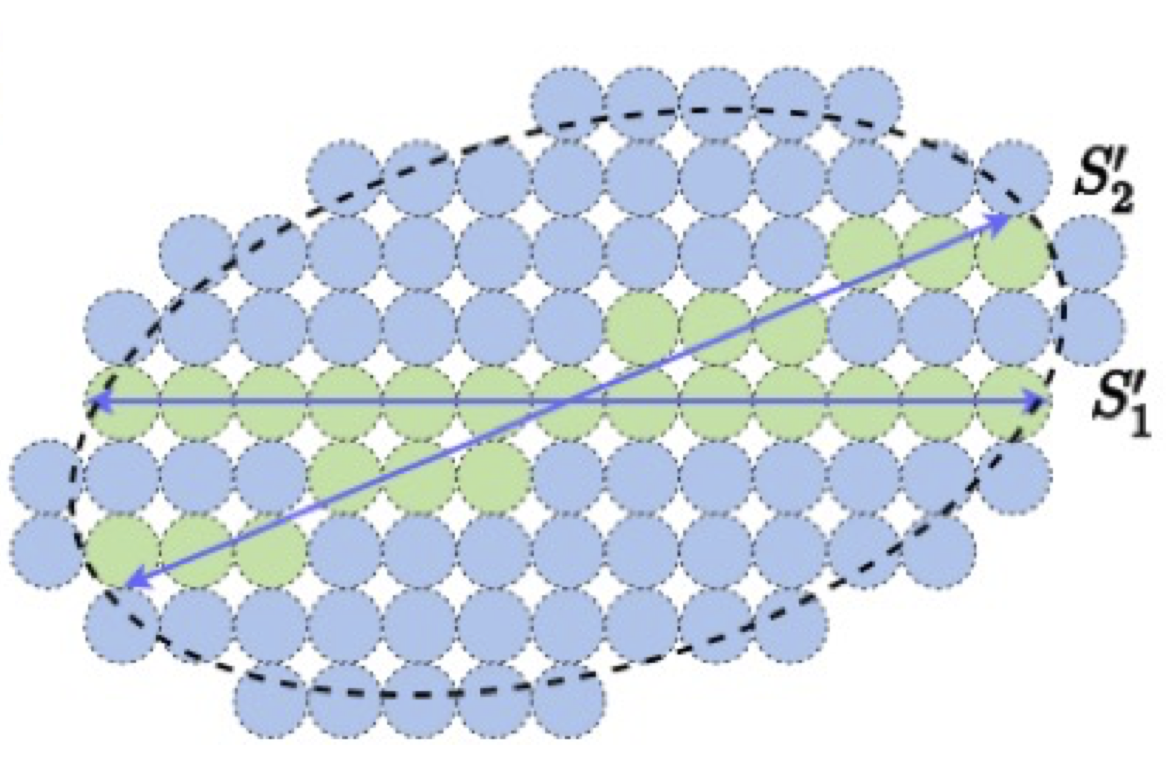
\includegraphics[width=0.5\linewidth]{\toplevelprefix/chapters/chapter1/figs/Coding-schemes.png}
    \caption{Comparison between two coding schemes. Image the true distribution of the data is around the two arrowed lines. One can code the samples from the two lines with the a code book consisting of all blue balls; one can also code the samples with a code book consisting of only the green balls. Obviously, the second coding schemes will result in much lower coding length/rate, subject to the same precision.}
    \label{fig:coding-schemes}
\end{figure}


Then the complexity of the predicting function $f$ can be evaluated as the average coding length of all sequences, known as the coding rate:\footnote{One may make this more precise by taking $R(f\mid \mathcal{E})$ to be the expected coding length for all segments of length $D$. }
\begin{equation}
   R(f \mid \mathcal E) = \mathbb{E}[L(\mathcal{E}(S))] \approx \frac{1}{N}\sum_{i=1}^N L(\mathcal{E}(S_i)). 
   \label{eqn:coding-rate}
\end{equation}
Obviously, the coding rate measure will change if one uses a different coding  scheme (or a code book). In practice, the better we know the low-dimensional structure around which the segments are distributed, the more efficient a code book we can design, as the example shown in Figure \ref{fig:coding-schemes}. Acute readers may have recognized that conceptually the denoising process illustrated in Figure \ref{fig:diffusion} resembles closely going from the coding scheme with the blue balls to that with the green ones.


Given two coding schemes $\mathcal{E}_1$ and $\mathcal{E}_2$ for the segments, if the difference in the coding rates is positive:
\begin{equation}
   R(f \mid \mathcal E_1) -  R(f \mid \mathcal E_2) > 0, 
\end{equation}
we may say the coding scheme $\mathcal{E}_2$ is better. This difference can be viewed as a measure of how much more information $\mathcal{E}_2$ has over $\mathcal{E}_1$ about the distribution of the data. To a large extent, the goal of learning $f$ is equivalent to finding the most efficient encoding scheme that minimizes the coding rate:
\begin{equation}
   \min_{\mathcal{E}} R(f \mid \mathcal E). 
\end{equation}
As we will see in Chapter \ref{ch:compression}, the achievable minimal rate is closely related to the notion of entropy $H(S)$ \eqref{eqn:entropy-definition}. 


\begin{remark}\label{rem:computable-complexity}
    {The perspective of measuring data complexity with explicit encoding schemes has motivated several learning objectives that were proposed to revise the Kolmogorov complexity for better computability \cite{WallaceC1999}, including the minimum message length (MML) proposed later in 1968 \cite{WallaceC1968} and the minimum description length (MDL) in 1978 \cite{Rissanen-1978,HansenM2001}. These objectives normally count the coding length for the coding scheme $\mathcal{E}$ itself (including its code book) in addition to the data $S$ of interest: $L(\mathcal E(S)) + L(\mathcal E)$.  However, if the goal is to learn a finite-sized code book and apply it to a large number of sequences, the amortized cost of the code book can be ignored since $$\frac{1}{N}\Big( L(\mathcal{E}) + \sum_{i=1}^N L(\mathcal{E}(S_i))\Big) \approx \frac{1}{N}\sum_{i=1}^N L(\mathcal{E}(S_i))$$ as $N$ becomes large.}
\end{remark}

Again, one may view the resulting optimal coding scheme as the one that achieves the best compression of the observed data. In general, compared to the Kolmogorov complexity, the coding length given by any encoding scheme will always be larger: 
\begin{equation}
    K(S) < L( \mathcal E(S)).
\end{equation} 
Therefore, minimizing the coding rate/length is essentially to minimize an upper bound of the otherwise uncomputable Kolmogorov complexity. 

\subsection{Learning Informative Representations}
%\paragraph{Structured representations via information gain.}
Note that if the goal was simply to compress the given data just for the sake of compression, then in theory the optimal codes that approach the Kolmogorov complexity would become nearly random or structureless \cite{Chaitin-1966}.\footnote{Because any codes with structures can be further compressed.} However, our true purpose of learning the predictive function $f$ is to use it repeatedly with ease in future predictions. Hence, while compression allows us to identify the low-dimensional distribution in the data, we would like to encode the distribution in a {\em structured and organized} way so that the resulting representation is very informative and efficient to use.\footnote{For example, to sample the distribution under different conditions.} Figure \ref{fig:expansion} shows an example that explains intuitively why such a transformation is desired. 

\begin{figure}
    \centering
    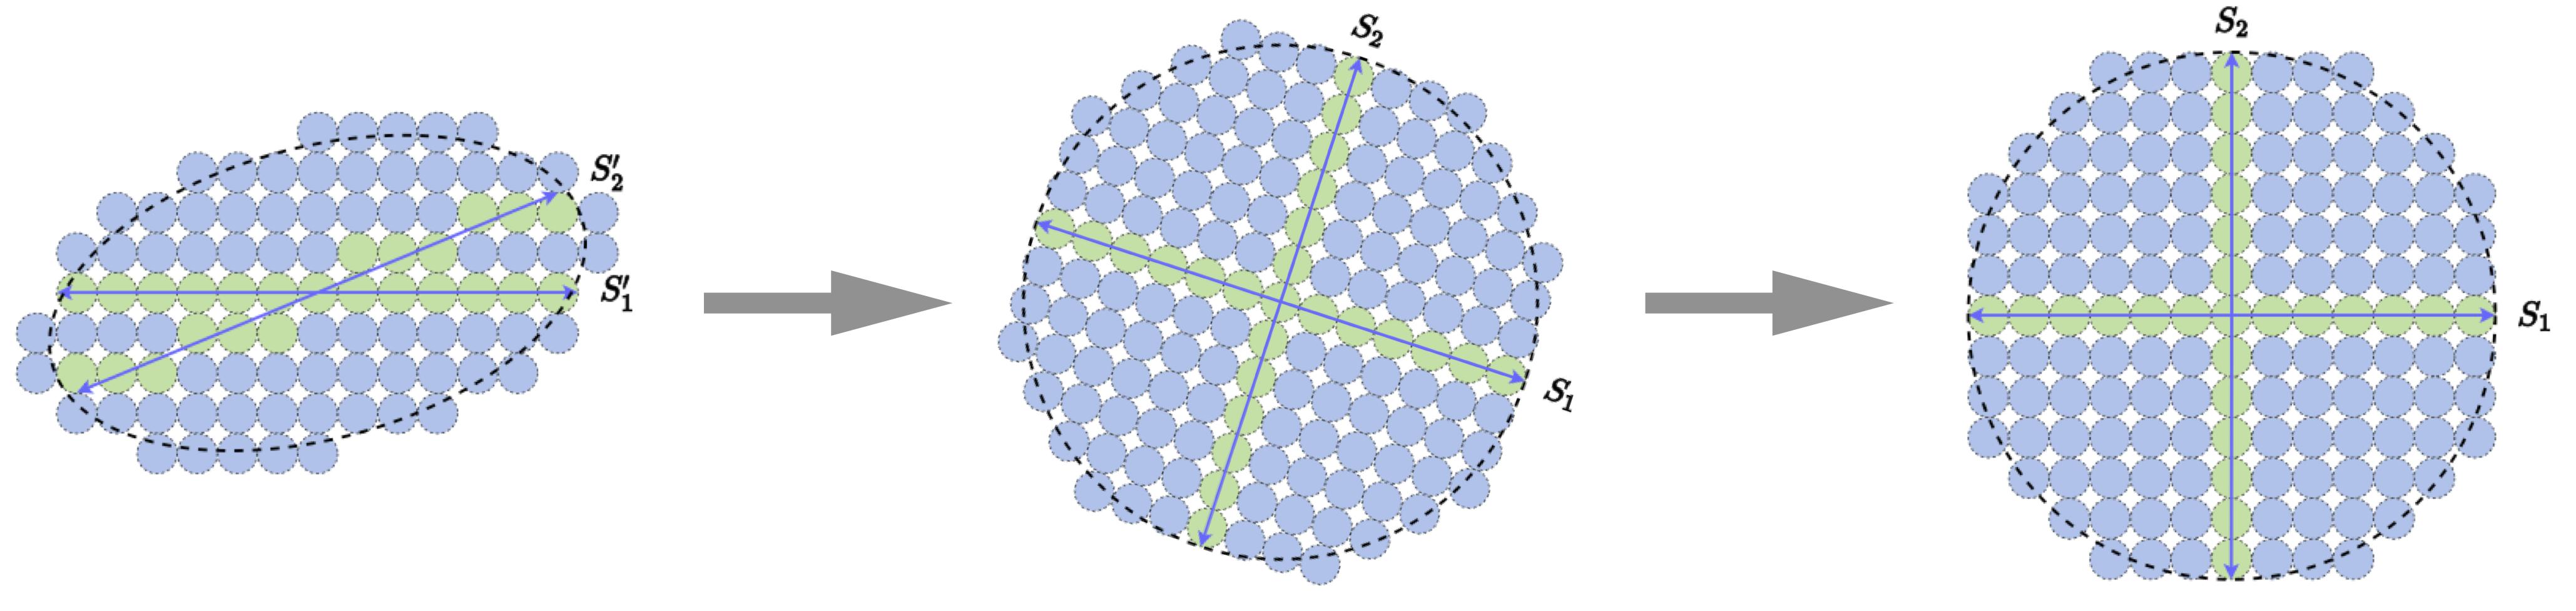
\includegraphics[width=0.98\linewidth]{\toplevelprefix/chapters/chapter1/figs/coding-transform.png}
    \caption{Transform the identified low-dimensional data distribution to a more informative and structured representation.}
    \label{fig:expansion}
\end{figure}
As we will show in Chapter \ref{ch:compression}, these desired structures in the final representation can be precisely promoted by choosing a natural measure of {\em information gain} based on the coding rates of the chosen coding schemes. As we see throughout this book, such an explicit and constructive coding approach provides a powerful computational framework for learning good representations of low-dimensional structures for real-world data, as in many cases of practical importance, the coding length function can be efficiently computed or approximated accurately. In some benign cases, we can even obtain closed-form formulae, e.g., subspace and Gaussian (see Chapter \ref{ch:compression}). 

In addition, such a computational framework leads to a principled approach that naturally reveals the role that deep networks play in this learning process. As we will derive systematically in Chapter \ref{ch:representation}, the layers of a deep network are trying to perform operations that optimize the objective function of interest in an incremental manner. From this perspective, the role of deep networks can be precisely interpreted as to emulate a certain iterative optimization algorithm, say gradient descent, to optimize the objective of information gain. Layers of the resulting deep architectures can be endowed with precise statistical and geometric interpretation, namely performing incremental compressive encoding and decoding operations. As a result, the derived deep networks become transparent ``white boxes'' that are mathematically fully explainable.  



% \textbf{Notes:} Convert predictability to low-dimensionality: A universal mathematical property of such data is that their distribution always has very low intrinsic dimensions, hence highly compressible, in the usually high-dimensional space they are embedded. 

% %Additional correlations that promote low-dimensionality, such as many physical laws described by partial differential equations, e.g. Maxwell equations for electric magnetic fields and Navier Stokes equations for fluid dynamics. 

% Measure of compactness: Many (largely equivalent) ways to measure compactness of data: Kolmogorov complexity (not computable), dimension and volume of (the support of) the data distribution, minimum description length, rate distortion etc. 

% Hence, one effective way to learn low-dimensional structures inherited from predictability is through certain operations of ``compression'' (which we will make precise later) that aim to minimize such measures. 





\subsection{Learning Consistent Representations}

%\subsection{Ensuring Consistency}
\label{sec:consistency}
To summarize our discussions so far, let us denote the data as:
\begin{equation}
    \boldsymbol{X} = \{S_1, S_2, \ldots, S_i, \ldots, S_N\} \subset \mathbb{R}^D,
\end{equation}
and let $\boldsymbol{Z} = \mathcal{E}(\X)$ be the codes of $\X$ via some encoder $\mathcal{E}$:
\begin{equation}
    \X  \xrightarrow{\hspace{2mm} \mathcal{E}\hspace{2mm}} \Z.
    \label{eqn:open-loop}
\end{equation}
In the machine learning context, $\Z$ is often called ``features'' or ``latent representation''. Note that without knowing the underlying distribution of $\X$, we do not know which encoder $\mathcal{E}$ should be that can retain most useful information about the distribution of $\X$. In practice, people often start with trying a certain compact encoding scheme that serves well for a specific task. In particular, they would try to learn an encoder that optimizes certain (empirical) measure of parsimony for the learned representation:
\begin{equation}
    \min \rho(\Z). 
\end{equation}

\begin{example}
For example, image classification is such a case: we assign all images in the same class to a single code and images in different classes to different codes, say ``one-hot'' vectors:
\begin{equation}
  \x \mapsto \z \in \{  [1, 0, 0, \ldots , 0, 0], \;  [0, 1, 0 \ldots, 0, 0], \; \ldots, \;  [0,0,0, \ldots, 0, 1].\}
  \label{eqn:class-labels}
\end{equation}
Now, a classifier $f(\cdot)$ can be modeled as a function that predicts the probability of a given $\x$ belonging to each of the $k$ classes: $\hat{\z} = f(\x) \in \mathbb{R}^K$. Then the ``goodness'' of a classifier can be measured by the so-called {\em cross entropy}:\footnote{The cross entropy can be viewed as a distance measure between the ground truth distribution of $\z$ and that of the prediction $\hat\z$. It can also be viewed as the expected coding length of $\z$ if we use the optimal code book for $\hat \z$ to encode $\z$. The cross entropy reaches minimum when $\z$ and $\hat \z$ have the same distribution.}
\begin{equation}
    L(\hat{\z}, \z) = \sum_{k=1}^K - z_k \log \hat{z}_k,
\end{equation}
where $z_k$ indicates the $k$-th entry of the vector $\z$. As the early practice of deep networks indicated \cite{krizhevsky2012imagenet}, if enough data are given, such an encoding scheme can often be represented by a deep network and learned in an end-to-end fashion by optimizing the cross-entropy. 
\end{example}

The cross-entropy loss $L(\hat \z, \z)$ can be viewed as a special measure of parsimony $\rho(\z)$ associated with a particular family of encoding schemes that are suitable for classification. However, such an encoding is obviously {\em very lossy}. The learned $\z$ does not contain any other information about $\x$ except for its class type. For example, by assigning an image with (a code representing) the class label ``apple'', we no longer know which specific type apple is in the original image from the label alone. 

Of course, the other extreme is to require the coding scheme to be {\em lossless}. That is, there is a one-to-one mapping between $\x$ and its code $\z$. However, as we will see in Chapter \ref{ch:compression},  lossless coding (or compression) is impractical unless $\x$ is discrete. For a continuous random variable, we may only consider lossy coding schemes so that the coding length for the data can be finite. That is, we only encode the data up to a certain prescribed precision. As we will elaborate more in Chapter \ref{ch:compression}, lossy coding is not merely a practical choice, it plays a fundamental role in making learning the underlying continuous distribution possible from finite samples of the distribution. 

For many purposes of learning, we want the feature $\z$, although {\em lossy}, to keep more information about $\x$ than just its class type. In this book, we will introduce a more general measure of parsimony based on coding length/rate associated with a more general family of coding schemes -- coding with a mixture of subspaces or Gaussians. This family has the capability to closely approximate arbitrary real-world distributions up to certain precision. As we will see in Chapter \ref{ch:compression} and Chapter \ref{ch:representation}, such a measure will not only preserve most information about the distribution of $\X$ but will also promote certain nice desired geometric and statistical structures for the learned representation $\Z$. 


\paragraph{Bidirectional Autoencoding for Consistency.}
In a broader learning context, the main goal of a compressive coding scheme $\mathcal{E}$ is to identify the low-dimensional structures in the data $\X$ so that they can be used to predict things in the original data space. This requires that the learned encoding scheme $\mathcal{E}$ allows an efficient decoding scheme, denoted as $\mathcal D$. It maps $\Z$, often known as a latent representation, back to the data space:
\begin{equation}
    \X   \xrightarrow{\hspace{2mm} \mathcal{E}\hspace{2mm}} \Z  \xrightarrow{\hspace{2mm} \mathcal{D} \hspace{2mm}} \hat \X.
       \label{eqn:auto-encoding}
\end{equation}
In general, we call such an encoding and decoding pair $(\mathcal{E}, \mathcal{D})$  an {\em autoencoding}. Figure \ref{fig:autoencoder}
illustrates the process of such an autoencoder. 
\begin{figure}
    \centering
    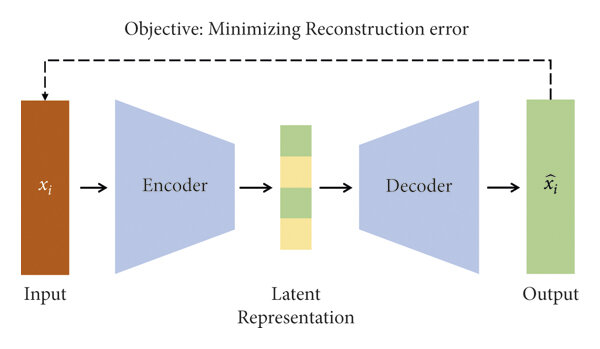
\includegraphics[width=0.7\linewidth]{\toplevelprefix/chapters/chapter1/figs/Autoencoder.jpg}
    \caption{Illustration of the architecture of an autoencoder. }
    \label{fig:autoencoder}
\end{figure}


Generally, we would prefer that the decoding is approximately an ``inverse'' to the encoding such that the data (distribution) $\hat \X$ decoded from $\Z$ would be similar to the original data (distribution) $\X$ to some extent.\footnote{We will make it more precise what we mean by being similar later.} If so, we would be able to recover or predict from $\Z$ what is going on in the original data space. In this case, we say the pair $(\mathcal{E}, \mathcal{D})$ gives a {\em consistent}  autoencoding. For most practical purposes, not only do we need such a decoding to exist, but also can be efficiently realized and physically implemented. For example, if $\x$ is a real-valued variable, quantification is needed in order for any decoding scheme to be realizable on a finite-state machine, as we will explain more in Chapter \ref{ch:compression}. Hence, in general, one should expect that realizable encoding and decoding schemes are necessarily lossy. A central question is how to learn a compact (lossy) representation $\Z$ such that it can be used to predict $\X$ well.

Generally speaking, as we will see, both encoder and decoder could be modeled and realized by deep networks and learned by solving an optimization problem of the following form:
\begin{equation}
   \min \, d( \X, \hat \X) + \rho(\Z), 
   \label{eqn:auto-encoding-objective}
\end{equation}
where $d(\cdot, \cdot)$ is a certain distance function that promotes similarity between $\X$ and $\hat \X$\footnote{Either sample-wise or distribution-wise similar, depending on the choice of the distance function $d$.} and $\rho(\Z)$ is some measure that promotes parsimony and information richness of $\Z$. The classic principal component analysis (PCA) \cite{JolliffeI2002} is a typical example of a consistent autoencoding, which we will study in great detail in Chapter \ref{ch:classic}, as a precursor to more general low-dimensional structures. In Chapter \ref{ch:autoencoding}, we will study how to learn consistent autoencoding for general (say nonlinear) low-dimensional distributions.  


\subsection{Learning Self-Consistent Representations}
Note that in the above autoencoding objective, one needs to evaluate how close or consistent the decoded data $\hat \X$ is to the original $\X$. This often requires some external supervision or knowledge on what similarity measure to use. Computing similarity between $\hat \X$ and $\X$ can be very expensive, if not entirely impossible or intractable.\footnote{Say one wants to minimize certain distributional distance between the two.} Note that in nature, animals are capable of learning all by themselves without comparing their estimate $\hat \X$ with the ground truth $\X$ in the data space. They typically do not even have that option. 

Then how is a system able to learn autonomously without external supervision or comparison? How can they know that $\hat \X$ is consistent with $\X$ even without directly comparing them? That leads to the idea of ``closing the loop''. As it turns out, under the mild conditions that we will make precise in Chapter \ref{ch:closed-loop}, to ensure $\X$ and $\hat \X$ are consistent, one only has to encode $\hat \X$ as $\hat \Z$ and check if $\Z$ and $\hat \Z$ are consistent. We call this notion of consistency as {\em self-consistency}, which  can be illustrated by the following diagram:
\begin{equation}
    \X   \xrightarrow{\hspace{2mm} \mathcal{E}\hspace{2mm}} \Z  \xrightarrow{\hspace{2mm} \mathcal{D} \hspace{2mm}} \hat \X \xrightarrow{\hspace{2mm} \mathcal{E}\hspace{2mm}} \hat \Z,
    \label{eqn:closed-loop}
\end{equation}
We refer to this process as a {\em closed-loop transcription},\footnote{Inspired by the transcription process between DNA and RNA or other proteins.} which is illustrated in Figure \ref{fig:closed-loop}.

\begin{figure}[t]
    \centering
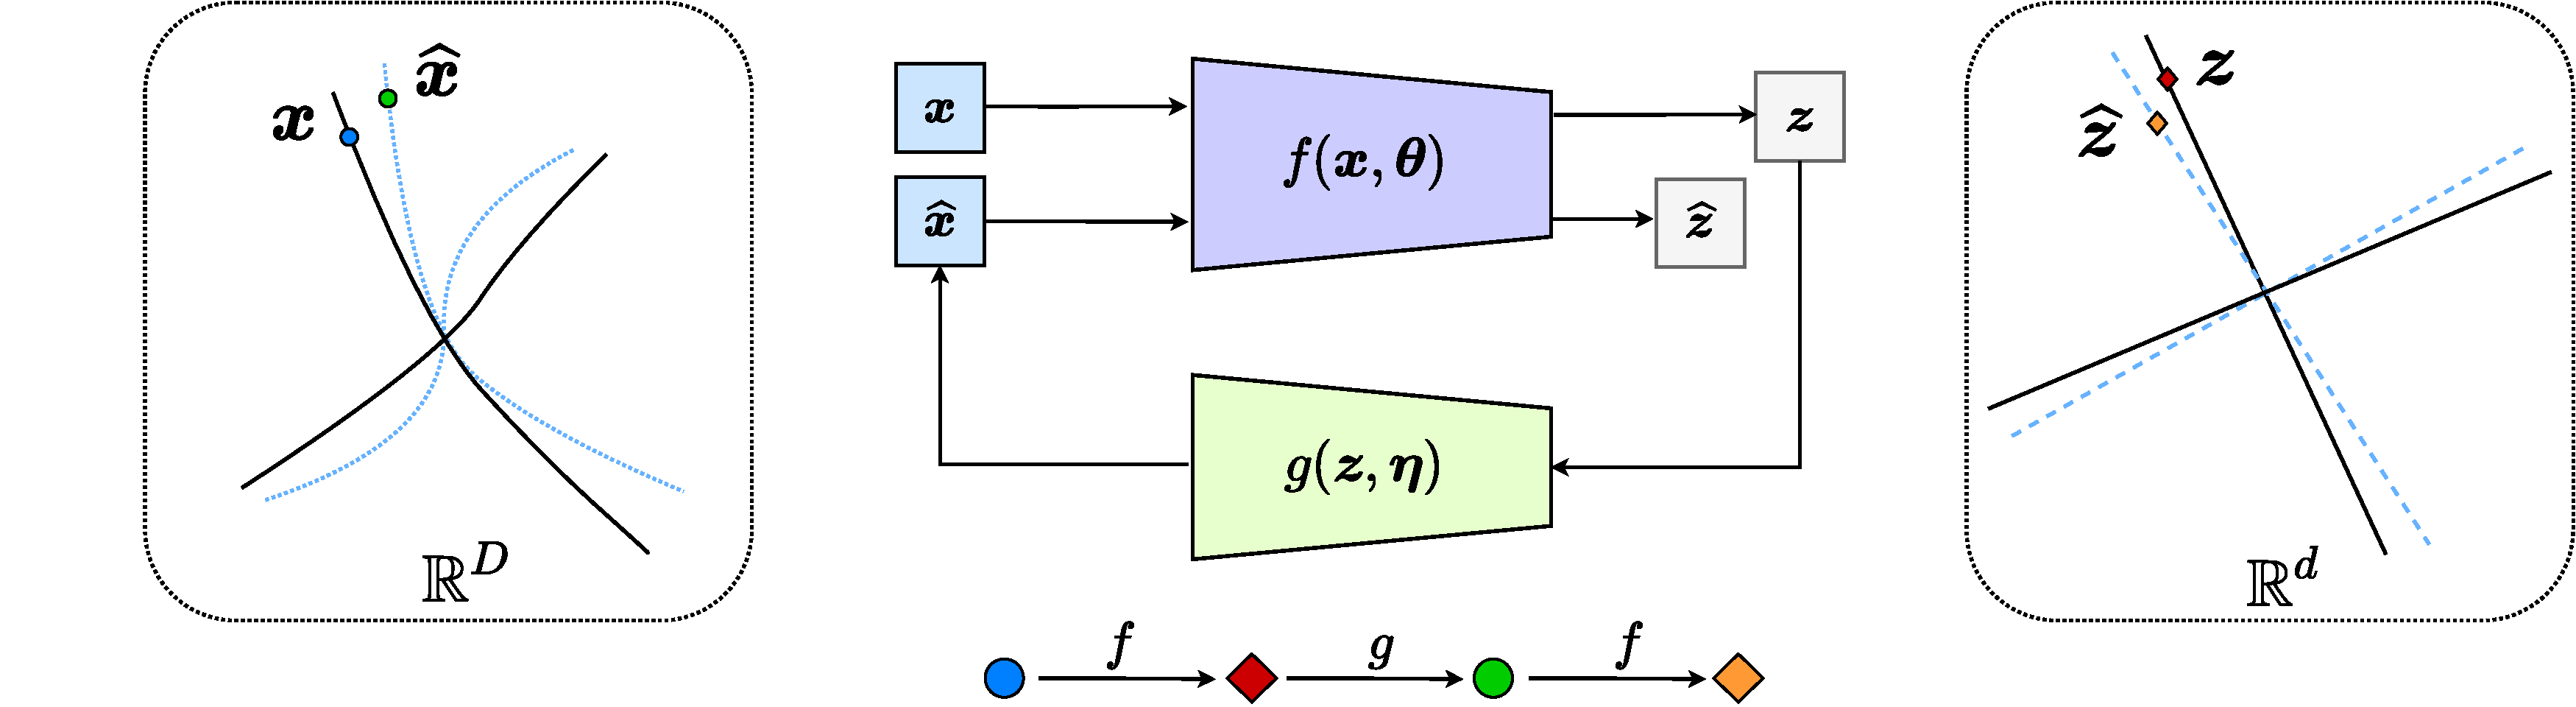
\includegraphics[width=0.9\linewidth]{\toplevelprefix/chapters/chapter1/figs/diagrams_redu_gan_2.pdf}
\caption{Illustration of a closed-loop transcription. Here we use a mapping $f$ to represent the encoder $\mathcal{E}$ and $g$ to represent the decoder $\mathcal{D}$.}  \label{fig:closed-loop}
\end{figure}

It is arguably true that any  autonomous intelligent being only needs to learn a self-consistent representation $\Z$ of the observed data $\X$, because checking consistency in the original data space (often meaning in the external world) is either too expensive or even not physically feasible. The closed-loop formulation allows one to learn an optimal encoding $f(\cdot, \theta)$ and decoding $g(\cdot, \eta)$ via a minmax game that depends only on the internal (learned) feature $\Z$:
\begin{equation}
\max_{\theta}\min_{\eta} \ell( \Z, \hat \Z) + \rho(\Z), 
   \label{eqn:closed-loop-objective}
\end{equation}
where $\ell( \Z, \hat \Z)$ is a loss function based on coding rates of the features $\Z$ and $\hat \Z$, which, as we will see, can be much easier to compute. Here again, $\rho(\Z)$ is some measure that promotes parsimony and information richness of $\Z$. Somewhat surprisingly, as we will see in Chapter \ref{ch:closed-loop}, under rather mild conditions such as $\X$ being sufficiently low-dimensional, self-consistency between $(\Z, \hat \Z)$ implies consistency in $(\X, \hat \X)$! In addition, we will also see that a closed-loop system will allow us to learn the distribution in a {\em continuous and incremental} manner,\footnote{That is to learn with one class at a time or even one sample at a time.} without suffering from problems such as catastrophic forgetting associated with open-loop models. 

\section{Bridging Theory and Practice for Machine Intelligence}
So far, we have introduced three related  frameworks for learning a compact and structured representation $\Z$ for a given data distribution $\X$: 
\begin{itemize}
\item The open-ended encoding \eqref{eqn:open-loop};
\item The bi-directional autoencoding \eqref{eqn:auto-encoding};
\item The closed-loop transcription \eqref{eqn:closed-loop}.
\end{itemize}
In this book, we will systematically study all three frameworks, one by one:
\begin{equation}
    \mbox{\textbf{open-ended}} \; \Longrightarrow \; 
    \mbox{\textbf{bi-directional}} \;  \Longrightarrow \; \mbox{\textbf{closed-loop}},
\end{equation}
in Chapter \ref{ch:representation}, \ref{ch:consistent}, and \ref{ch:closed-loop}, respectively.

In the past few years, many theoretical frameworks have been proposed and developed to help understand deep networks. However, many were unable to provide scalable solutions that matched the performance of empirical methods on real-world data and tasks. Many theories do not provide useful guidance on how to further improve practice. Chapters \ref{ch:conditional-inference} and  \ref{ch:applications} will show how the framework presented in this book may help bridge the gap between theory and practice. Chapter \ref{ch:conditional-inference} will show how to use the learned distribution and its representation to conduct Bayesian inference for practical tasks that depend on conditional estimation and prediction. Chapter \ref{ch:applications} will provide convincing experimental evidence that networks and systems designed from the first principles can achieve competitive and potentially better performance on a variety of tasks such as visual representation learning,  image classification, image completion, segmentation, and text generation.


\paragraph{Back to intelligence.}
As we have mentioned in the beginning, a fundamental task of any intelligent being is to learn predictable information from its sensed data. Now we have understood a little about the computational nature of this task, and one should realize that this is a never-ending process, for the following reasons:
\begin{itemize}
    \item The current learned knowledge from the data, say the encoding and decoding schemes, can never really be optimal. Intelligence should have the ability to improve if there are still errors in predicting new observations. 
    \item The data observed so far do not yet cover all the predictable information. Intelligence should be able to recognize that current knowledge is inadequate and have the capability to learn and acquire new information.
\end{itemize}

Hence, intelligence is {\em not} about simply collecting all data in advance and training a model to memorize all the predictable information in the data. In contrast, it is about being equipped with computational mechanisms that can constantly improve current knowledge and acquire new information when needed. That is, a fundamental characteristic of any intelligent being or system\footnote{An animal, a human being, an intelligent robot, the scientific community, and even the entire civilization.} is {\em being able to continuously improve or gain information (or knowledge) on its own}. Conceptually, we may illustrate the relationship between intelligence and information (or knowledge) as follows:
\begin{equation}
\operatorname{Intelligence}(t) = \odv*{\operatorname{Information}}{t}(t), \qquad 
\operatorname{Information}(t)  = \int_0^t \operatorname{Intelligence}(s) \odif{s}.
\end{equation}
We believe that the closed-loop framework is a universal mechanism that enables self-improving and self-learning, via feedback and gaming. All intelligent beings or systems in nature utilize closed-loop mechanisms for learning at all levels and on all scales. Its ubiquity had inspired early studies that tried to model and emulate animal intelligence by machines and computers, particularly the Cybernetics movement initiated by Norbert Wiener in the 1940s. We hope that this book will help people better understand the objectives, principles, and computational mechanisms behind intelligence. It may serve as a foundation for a deeper study of higher-level human intelligence in the future, which we will discuss more at the end of the book in Chapter \ref{ch:future}.

\end{document}
